\documentclass[onehalfspacing,reservepages,10pt]{sjvanschaik-thesis}

\usepackage[english]{babel}
\usepackage{mathptmx}
\usepackage{amsfonts}
\usepackage{amsmath}
\usepackage{amssymb}
\usepackage{amsthm}
\usepackage{graphicx}
\usepackage{times}
\usepackage{flushend}
\usepackage{enumitem}
\usepackage{graphicx}
%\usepackage{program}

\newcommand{\lt}{<}
\newcommand{\gt}{>}

\ThesisAuthor{Eamonn J. Maguire}
\ThesisCollege{St. Anne's College}
\ThesisTitle{Compression in Visualization}
\ThesisTerm{Michaelmas}
\ThesisYear{2014}

% TODO:
\ThesisKeywords{{visualization}; {compression}}

\begin{document}

\frontmatter
\maketitle

\begin{romanpages}
%\ThesisAbstract{%
The digitalisation of information now affects most fields of human activity.
From the social sciences to biology to physics, the volume, velocity, and variety of data exhibit exponential growth trends.
With such rates of expansion, efforts to understand and make sense of datasets of such scale, however driven and directed, progress only at an incremental pace.
The challenges are significant.
For instance, the ability to display an ever growing amount of data is physically and naturally bound by the dimensions of the average sized display.
A synergistic interplay between statistical analysis and visualisation approaches outlines a path for significant advances in the field of data exploration.
We can turn to statistics to provide principled guidance for prioritisation of information to display.
Using statistical results, and combining knowledge from the cognitive sciences, visual techniques can be used to highlight salient data attributes.

The purpose of this thesis is to explore the link between computer science, statistics, visualization, and the cognitive sciences, to define and develop more systematic approaches towards the design of glyphs.

Glyphs represent the variables of multivariate data records by mapping those variables to one or more visual channels (\eg, colour, shape, and texture).
They offer a unique, compact solution to the presentation of a large amount of multivariate information.
However, composing a meaningful, interpretable, and learnable glyph can pose a number of problems.
The first of these problems exist in the subjectivity involved in the process of data to visual channel mapping, and in the organisation of those visual channels to form the overall glyph.
Our first contribution outlines a computational technique to help systematise many of these otherwise subjective elements of the glyph design process.

For visual information compression, common patterns (motifs) in time series or graph data for example, may be replaced with more compact, visual representations.
Glyph-based techniques can provide such representations that can help users find common patterns more quickly, and at the same time, bring attention to anomalous areas of the data.
However, replacing any data with a glyph is not going to make tasks such as visual search easier.
A key problem is the selection of semantically meaningful motifs with the potential to compress large amounts of information.
A second contribution of this thesis is a computational process for systematic design of such glyph libraries and their subsequent glyphs.

A further problem in the glyph design process is in their evaluation.
Evaluation is typically a time-consuming, highly subjective process.
Moreover, domain experts are not always plentiful, therefore obtaining statistically significant evaluation results is often difficult.
A final contribution of this work is to investigate if there are areas of evaluation that can be performed  computationally.
}
\Abstract

%\begin{dedication}
Dedicated to my Mum.
\end{dedication}

%\begin{acknowledgements}

\noindent I'm in so much debt to many people who have been part of this enjoyable journey, but first and foremost I would like to thank my supervisors Prof. Min Chen, Prof. Jim Davies and Dr. Susanna-Assunta Sansone. 


To Min Chen who took me as a raw DPhil student and through his support, patience, guidance, and endless energy has helped guide me through the entire process. 
It has been a great pleasure to work with someone held in such high esteem by the visualization community and I am so fortunate to have been given the chance to conduct my DPhil with him.


To Susanna-Assunta Sansone who has given me the freedom to pursue a DPhil whilst conducting research and the Oxford e-Research Centre (OeRC) for supporting this process. 
We have worked together for six years now, and I have enjoyed being in her growing group and seeing things go from strength to strength.

To Philippe Rocca-Serra who has also put up with me for six years now, interspersed with my delightfully accurate French accent. 
Philippe is a great friend who has been a tremendous support through all stages of this journey, in particular the more difficult ones. 

To Annapaola Santarsiero who has dealt with the many late nights and weekend work for three years whilst always being supportive.
Annapaola even agreed to marry me when I proposed during the writing up process!

Additionally, I owe a great deal to my incredibly talented friends and colleagues at the OeRC who have made my time in Oxford so great.
Their knowledge, passion, friendliness, and availability to share their knowledge has been amazing.
In particular I wish to thank Alejandra González-Beltrán, Simon Walton, Alfie Abdul-Rahman, Brian Duffy, Endre Lászió, Piotr Łopatka, Ramon Granell, Raz Lakhoo, Stef Salvini, Istvan Reguly, Ségolène Tarte (who also endured my French accents), Milo Thurston, Neil Caithness, Bas van Schaik, Kay Sutton, Ross McCartney, Clem Harris, and David DeRoure. 

Finally to my great network of friends in Oxford and beyond who have all in some way played a part in my journey, including Tommy Barr, Ryan McCrea, David Close, Liam Kelly, Matt Brinklow, Devan Govender, James Malone, Will McClaren, Rasmus Wissman, Sam Whitehead, Chris Boddy, Dan Short, Ian Robertson, Caterina Doglioni, and so many more!

I would also like to thank and remember the contributions of Professor Matthew Ward who researched glyphs extensively and contributed a large amount of knowledge in the direction of glyph-based visualization.
Professor Ward was to present with Dr. Rita Borgo, Prof. Min Chen, and Prof. Sine McDougall at the glyph tutorial at VIS 2014 in Paris, but sadly passed away in October 2014.

\end{acknowledgements}
   

%set the number of sectioning levels that get number and appear in the contents
\setcounter{secnumdepth}{3}
\setcounter{tocdepth}{3}

{\fontsize{12pt}{14pt}\selectfont\tableofcontents} 

\end{romanpages}

\mainmatter

%\chapter{My Chapter}
%\blindtext
\chapter{Introduction}
\label{chap:introduction}

In an article published in 2002, Matt Ward stated that data sizes were exploding \cite{ward02}.
Since then, the rate of data growth has not relented.
Facebook, Twitter, LinkedIn, and Google Plus, all of which did not exist in 2002, contribute huge amounts of information to government departments, marketers, and social scientists.
The democratisation of DNA sequencing technology combined with a scientific need to bring together many different data sources in to their analyses (\eg, RNA, proteomic, metabolomic, and clinical chemistry data) has pushed the biological sciences into a more data-centric domain.
Since 2008, physicists can now get their hands and algorithms on over 20 petabytes of information every year from the large hadron collider at CERN.
By bringing together lots of information from different sources, it is commonplace for a data record to have anything from tens to thousands of quantitative and qualitative data variables (termed multivariate data) \cite{ward02}.

So how does one deal with such data and interpret it?
Statistical techniques are effective in the detection of trends and outliers in data where there is a pre-existing model of what is expected.
However, they are not so effective in the detection of trends and outliers in data when no such model exists.
The human perceptual system is incredibly powerful at finding patterns or outliers that statistical techniques may miss.
When no model is yet known or unavailable, or when uncertainty exists on an underlying model, visualization can take advantage of the human perceptual system to help users in a number of tasks, including:
\begin{enumerate}
\item observation of trends and outliers;
\item creating connections between data and past experience, knowledge, and intuition;
\item visual generation and evaluation of hypotheses;
\item monitoring the correctness and performance of computational models; and 
\item effective communication with others.
\end{enumerate}

\begin{figure}[t!]
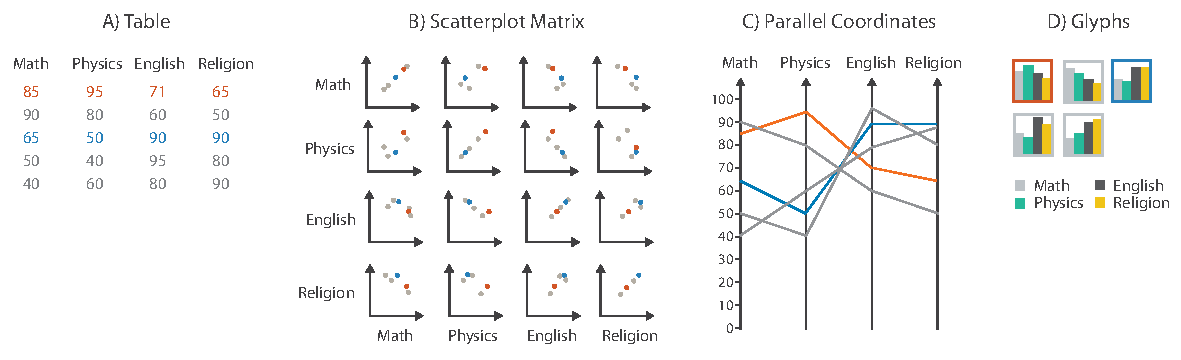
\includegraphics[width=\textwidth]{images/introduction/multivariate_vis}
\caption{Techniques for multivariate data exploration include: A) tables; B) scatter plot matrices (SPLOMS); C) parallel coordinate plots; and D) glyph-based visualization.}
\label{fig:multivariate_vis}
\end{figure}

Multivariate data visualization is a class of visualization techniques that deal with the presentation of many data record attributes at once.
Four primary multivariate data visualization techniques displayed in Figure \ref{fig:multivariate_vis} are:

\begin{enumerate}
\item \textbf{Data Tables} (Figure \ref{fig:multivariate_vis} A) are the simplest and most pervasive form of visualization.
There are many limitations to tables over more graphical visualization techniques generally around scalability (you can only view a limited number of rows at a time), and trend/outlier identification problems (it is hard to see large scale trends in a table);

\item \textbf{Scatter plot matrices (SPLOMS)} (Figure \ref{fig:multivariate_vis} B) where each dimension of a record is plotted against other dimensions \cite{Elmqvist2008Scatter} as an individual scatter plot.
This technique suffers in that $N^2$ plots are required where $N$ is the number of dimensions.
So while this technique is effective for a small number of dimensions, its capabilities diminish as the number of dimensions grow; 

\item \textbf{Parallel coordinate plots} (Figure \ref{fig:multivariate_vis} C) encode each variable/dimension of a data record as an axis with a line passing through each axis at the point given by the data record.
A full review of parallel coordinates can be found in a STAR from Heinrich and Weiskopf \cite{heinrich2012state}; and

\item \textbf{Glyph-based visualization} (Figure \ref{fig:multivariate_vis} D) uses visual items (termed glyphs) to encode data attributes using a number of visual channels (\eg, colour, shape, size, position, etc.).
These glyphs can then be positioned independently in 2D or 3D space to form the overall visualization.
\end{enumerate}


\section{Glyph-based Visualization Challenges}
While tables, SPLOMs and parallel coordinate plots can be deployed relatively easily, \emph{effective} glyph-based solutions are generally more difficult to implement.
Glyph-based visualization is a powerful technique, offering an advantage over other multivariate data visualization techniques in their ability to preserve spatial information.
However, their implementation is not straightforward and a number of challenges exist within information visualization (largely 2D) and scientific visualization (largely 3D).
Drawing from the State of the Art Report (STAR) on glyph-based visualization from Borgo \etal \cite{Borgo:2013:EG}, and Matt Ward's paper on ``Multivariate Data Glyphs: Principles and Practice'', the following challenges can be extrapolated:


\begin{enumerate}
\item \textbf{Technical Challenges}:
	\begin{enumerate}
		\item \textbf{Challenge 1} - \emph{Glyph Placement} concerns how glyphs are arranged spatially in 2D or 3D scenes.
		Position is an important visual channel, therefore ensuring glyphs are displayed in the right position is a key problem in many domains.
		
		Matt Ward's excellent survey on glyph placement provides a great overview of a number of strategies for glyph placement that includes data- and structure-driven techniques \cite{ward02}.
		Ropinski \cite{ropinski11} added a further strategy for medical data, named feature-driven glyph placement which places glyphs on particular features of the underlying data.
		Borgo \etal \cite{Borgo:2013:EG} also added user-driven glyph placement as a categorisation.
		Glyph placement remains a problem within the visualization community due to problems with occlusion for example.
		
		\item \textbf{Challenge 2} - \emph{Data Ordering} considers how data records can be ordered or have sets of variables grouped to highlight specific trends or interesting parts of the data\cite{ward08}.
		The ordering of the underlying data can influence how particular features of the data are interpreted during analysis and is very much task dependent.
		For example, if a user is using a glyph-based visualization to gain an overview of how much customers have spent over the past year, having randomly ordered monthly totals is not going to be as useful as having the months arranged naturally from January to December.
		
		\item \textbf{Challenge 3} - \emph{Glyph-based Visual Compression} is a technique that uses glyphs to reduce the amount of visual space taken up in a display by common patterns/motifs.
		A key challenge in this technique is determining which parts of the data are not only common, but will also visually compress the most space.
		Additionally, instead of ad-hoc compressions of data, a further challenge would be in creating glyph libraries to be used across a domain to consistently represent common features in their data.
		
	\end{enumerate}
\item \textbf{Design Challenges}:
	\begin{enumerate}
			\item \textbf{Challenge 4} -  \emph{Data to Visual Mapping} relates to how particular data variables are mapped to colour, shape, size, and texture for example (called visual channels).
			Mappings can vary depending on the type of the data variable (\eg, categorical or quantitative) with not all visual channels being equally good or bad at representing either type of variable.
			Challenges exist in determining which data items should be represented by which visual channels.
			For example, some visual channels are perceived together (integrally) rather than separately.
			The result is two data variables being mapped to integral visual channels, thereby hiding aspects of the original data record.
			Additionally, colour is a powerful visual channel, while texture is not.
			How can a glyph designer decide over whether to use colour for one variable, and texture for the other?
			
			\item \textbf{Challenge 5} - \emph{Glyph Arrangement} refers to how a glyph will arrange its constituent parts.
			This is often required for more complex glyphs that are representing many dimensions.
			For example, in Chernoff faces various data values are mapped to facial features such as face, nose, and eye dimensions.
			In this case, the arrangement of glyph features is given due to the natural ordering of facial features, but this is not always the case.
			
			This relates to glyph distinguishability which is concerned with how glyphs are perceived at different resolutions.
			By ensuring that variables important to the user tasks are available when glyphs are small, users will be able to use many glyphs on a screen at once, and visually filter for glyphs representing data items of interest.
			
			A key challenge for glyph arrangement is in the provision of more systematic methods for deciding how visual channels can be composed to form a glyph.
			
	\end{enumerate}
	
\item \textbf{Evaluation Challenge}:
\begin{enumerate}
	\item \textbf{Challenge 6} - \emph{Quality Measurement}. Numerous examples of glyph-based visualization are applied to the medical domain.
	In such domains, obtaining enough attention from a domain expert (a doctor or consultant) in order to carry out a meaningful evaluation is difficult.
	It is therefore hard to fully evaluate glyph \emph{memorability}, \emph{distinguishability}, \emph{interpretability}, and \emph{utility} of a glyph set.
	Therefore a key challenge is in finding ways other than through user interaction, to assess typical evaluation metrics.
\end{enumerate}

\end{enumerate}

In this thesis, we investigate a number of these technical, design, and evaluation challenges of glyph-based visualizations through the provision of a more systematic process towards glyph design .
This systematic process largely involves the heavy use of computational techniques (accompanied by design principles) to investigate the following three questions:

\begin{enumerate}
\item \textbf{Is glyph design amenable to systematization by computational methods?}
How can one go from data values to a visual channel, and how can these channels be organised in to a coherent glyph?
Well-designed glyphs can greatly enhance visual search and pattern identification, and are intuitive to learn and use.
However, as Ward stated, the selection of one visual channel over another could have direct implications on how an attribute is perceived and interpreted by an observer \cite{ward02}.
For example, some visual channels are better at representing qualitative information while others are better at representing quantitative information.
Additionally, glyphs are often small, therefore visual channels will have relatively limited bandwidth capacities.
How can a glyph be designed to ensure that important information is visually accessible to users?

This question investigates \textbf{Challenges 2, 4, and 5} from the glyph challenges stated above.


\item \textbf{Can computational methods be applied to the design of glyph libraries for visual compression?}
A further application area for glyphs is in the visual compression of information.
Most displays will have a screen width of approximately two thousand pixels.
This means that for time series data for example, you can plot two thousand values (considering no need for connecting lines) before having to sample the data.
If common patterns in the data (motifs) were represented as a glyph library, the data could be compressed, leaving the ``interesting'' parts of the data in a more digestible form for users.
The question is, how can such a glyph library be designed?
In some domains, common patterns may be known by domain-experts, and this could form the basis of the glyph library.
In other domains, the library will evolve as a result of many years of refinement.
In other domains however, little may be known, so how can decisions be made on which data should be represented by glyphs?
Can computation play a role in controlling this process?

This question investigates \textbf{Challenge 3} from the glyph challenges stated above.

\item \textbf{Are there areas of evaluation that can be performed more systematically?}
Evaluation is normally carried out by human observers in time-consuming studies.
The results and impact of such studies can be limited by the number of domain experts.
We wish to investigate how evaluation can be made more systematic and whether computation can replace humans in some aspects of glyph evaluation.

This question investigates \textbf{Challenge 6} from the glyph challenges stated above.

\end{enumerate}

\section{Thesis Scope}
The scope of this thesis falls within the greater subject area of Computer Science, specifically \emph{Computer Science} $\rightarrow$ \emph{Visual computing} $\rightarrow$ \emph{Visualization} $\rightarrow$ \emph{Information visualization} and \emph{Visual analytics} $\rightarrow$ \emph{Glyph-based, high-dimensional visualization}.


Visualization as a domain is spanned across two major areas.
These areas, defined by the freedom to choose where elements are spatially positioned in a visualization are as follows:

\begin{enumerate}
	\item \textbf{Scientific Visualisation (SciVis)} is built upon the underlying premise that spatial position is \emph{given} within the data set \cite{munzner2014visualization, telea2014data}.
	This means that visualization designers do not have a choice in where to position elements.
	The majority of \emph{SciVis} contributions are therefore spatial data visualizations.
	
	\item \textbf{Information Visualisation (InfoVis)} concerns visualization challenges where the use of space is \emph{chosen} by the visualization designer \cite{munzner2014visualization}.
	Due to the choices involved, and the subjectivity often present in making these choices, the domain of \emph{InfoVis} is largely concerned with determining whether of not the chosen design is fit for purpose, hence the design studies and evaluations that populate the \emph{InfoVis} category.  
\end{enumerate}

Additionally, Visual analytics (extensively featured in the Visual Analytics Science and Technology (VAST) Conference at IEEE VIS) is a relatively new field that spans the \emph{scientific} and \emph{information visualization} domains.
Visual analytics is often defined as the``integration of analysis, visualization and interaction".
The benefit of this paradigm is that visual analytics brings together the processing capabilities of computers and the pattern recognition, and hypothesis generating capabilities of humans.


Furthermore, additional research venues are appearing that encompass domain-specific groupings of visualizations that are somewhat free of the \emph{SciVis}, \emph{InfoVis}, and \emph{VAST} categorisations.
For example, in biology there is BioVis (\url{http://www.biovis.net/}), and for security there is VisSec (\url{http://www.vizsec.org/}).

The work presented in this thesis has solely focuses on \emph{information visualization} and \emph{visual analytics} with application areas in biology and security.

\section{Thesis Organization and Contributions}
The thesis from hereon in is organised into seven chapters that collectively aim to answer the above questions. 

\textbf{Chapter \ref{chap:related_work}} provides a detailed view of the psychology literature describing the various properties of the human visual system and how this can be exploited in glyph design.
We follow with an overview of the large body of research in glyphs from their origins to their present day use.
The latter part of this chapter is based upon a STAR report co-authored with Borgo \etal \cite{Borgo:2013:EG}. 

\textbf{Chapter \ref{chap:strategies}} proposes a model representing a more systematic glyph design process.
This model will be applied throughout the thesis to determine its applicability to a number of glyph-based visualization challenges.

\textbf{Chapter \ref{chap:glyph-tax}} details a systematic way of creating glyphs using a taxonomy-based approach for the replacement of text labels in biological workflows. 
This work addresses a number of technical and design glyph-based visualization challenges.
First we provide a novel solution to a technical challenge through algorithmic creation of a taxonomic tree for \emph{Challenge 2 - Data Ordering}.
This involved the creation of a novel algorithm for the classification of a large corpus of qualitative data to create a balanced tree.

We then proceed to address two design challenges.
Visual channels are ordered by their strength and a number of perceptual guidelines are highlighted which relates to \emph{Challenge 4 - Data to Visual Mapping}.
This ordering is based on a large review of the psychology literature on human perception from Chapter \ref{chap:related_work}.

Finally, we propose a solution to \emph{Challenge 5 - Glyph Arrangement} by using the taxonomic tree to guide the creation of glyphs.
The top level of the tree is represented by the strongest visual channels, and the lowest levels of the tree are represented by the least prominent visual channels.
We propose a test for the final glyph arrangement via a ``crush'' test that can be used to determine whether or not the important information in the glyph is available to observers even at low resolutions.


This work was published in IEEE TVCG in a publication by Maguire \etal \cite{Maguire:2012:TVCG} and presented in the InfoVis track at IEEE VIS 2012.
Additionally, the basis of this work forms a key component of the IEEE VIS 2014 tutorial on glyph-based visualization\footnote{\url{http://ovii.github.io/IEEEVisGlyphTutorial/}}. 
This work was jointly performed with Philippe Rocca-Serra, Susanna-Assunta Sansone, Jim Davies and Min Chen.  
The implementation and paper writing was conducted by Eamonn Maguire, Min Chen guided the work, and Philippe Rocca-Serra, Susanna-Assunta Sansone, and Jim Davies provided further domain knowledge and validated the technique.\\

\textbf{Chapters \ref{chap:automacron}} and \textbf{\ref{chap:timeseries}} investigate how computation can help in the design of glyph libraries for visual compression.
Both chapters investigate a technical glyph-based challenge in \emph{Challenge 3 - Glyph-based Visual Compression} for two data types, graph and time series data respectively.\\

\textbf{Chapter \ref{chap:automacron}} investigates the compression of workflow visualizations introduced in Chapter \ref{chap:glyph-tax} with automatically created glyphs.
This involves the creation of a novel frequent pattern (motif) finding algorithm for directed acyclic graphs.
This algorithm advances on previous algorithms through the ability to discriminate between types of nodes and edges in motifs.
By running the algorithm over 10,000 workflows, we can determine the common motifs.
Glyphs are automatically created for the most common motifs to form a library of `macro' glyphs, similar in concept to macros used in electronic circuit diagrams for example.
The resulting glyph library is used to visually compress biological workflows. 

This work was published in IEEE TVCG in a publication by Maguire \etal \cite{maguire13} and presented in the InfoVis track at IEEE VIS 2013.
The work was jointly performed with Philippe Rocca-Serra, Susanna-Assunta Sansone, Jim Davies and Min Chen.  
Implementation, and paper writing was conducted by Eamonn Maguire, Min Chen guided the work, Philippe Rocca-Serra, Susanna-Assunta Sansone, and Jim Davies provided domain knowledge to validate the technique.\\

\textbf{Chapter \ref{chap:timeseries}} builds on the research presented in Chapters \ref{chap:glyph-tax} and \ref{chap:automacron} with the use of glyphs for the visual compression of time series data.
We present a novel algorithm to find frequent long patterns (FLPs) or motifs in a corpus of time series data. 
This algorithm can be refined using a visual analytics platform required due to the parameter tuning required for different data domains.
Resulting motifs are automatically represented by glyphs, and these are used to visually compress a time series, leaving anomalous regions in place.
The work was jointly performed with Susanna-Assunta Sansone, and Min Chen.
Implementation was conducted by Eamonn Maguire, Susanna-Assunta Sansone helped in presenting some biological use cases, and Min Chen guided the work.\\

\textbf{Chapter \ref{chap:processes}} presents a number of glyph design processes and evaluation methods in addition to those used in the Chapters \ref{chap:glyph-tax} to \ref{chap:timeseries}. These processes and evaluations have been applied to three diverse cases: 
\begin{enumerate}

\item \textbf{Biological sequence visualization (DNA, RNA, and amino acid)} which focuses on the improvement of an existing design for visualization of biological sequence ``logos'' that show areas of DNA/amino acid conservation across different species.
We create a new glyph to represent conservation at each position in a sequence, and add additional glyphs to help users interpret why these changes happen.

This work investigated how much of the perception research gathered throughout the thesis could be used to improve a visualization.
This relates to challenges \emph{Challenge 4 - Data to Visual Mapping} and \emph{Challenge 5 - Glyph Arrangement}.
We investigated how the existing ``sequence logo'' visualization could be improved to improve data interpretation by considering research presented in Chapter \ref{chap:related_work}, especially that relating to spatial frequencies and global/local processing.
Additionally, by ordering the arrangement of elements within the glyph, we aimed to further improve the interpretation of our results.
An online evaluation encompassing over forty bioinformaticians and biologists confirmed that our approach had improved interpretation.

The work was published as a short paper and presented at EuroVis 2014 in a paper entitled \emph{Redesigning the Sequence Logo with Glyph-based Approaches to Aid Interpretation} \cite{CGF:maguire14-sp}.
The design, implementation, and paper writing were performed by Eamonn Maguire.
Design options discussed with Susanna-Assunta Sansone, Philippe Rocca-Serra, and Min Chen;

\item \textbf{Poetry visualization} where we present two pieces of work focusing on glyph-based solutions for poem visualization.
The first focuses on the design of a representation for twenty-six poem variables. 
This work was performed with: Alfie Abdul-Rahman who performed requirements elicitation, implemented the software, and conducted evaluations; Min Chen who led the project; numerous researchers from Oxford and Utah who participated in the requirements gathering and evaluation processes; and Eamonn Maguire who designed the poem glyphs.

This work presents a solution to \emph{Challenge 4 - Data to Visual Mapping} through the provision of a user-driven approach to data mappings between data and their respective visual encoding.
The rule-based approach applied to this mapping process provides some assurances over the quality of mappings, by ensuring users do not choose unsuitable mappings or overload the use of particular visual channels.

This work was published in the Computer Graphics Forum in 2013 in a publication by Abdul-Rahman \etal named \emph{Rule-based Visual Mappings -- with a Case Study on Poetry Visualization} \cite{CGF:Abd2013a}.
 
The second focuses on the design of a ``macro'' glyph to show the changes in the sounds of each line of a poem.
This work presents a solution to \emph{Challenge 5 - Glyph Arrangement} through the use of statistical data analyses to inform the ``macro'' glyph design.

This work was performed with: Alfie Abdul-Rahman who performed requirements elicitation, participated in the glyph design process through performing a statistical analysis of the data, and conducted evaluations; Min Chen who led the project; and Eamonn Maguire who worked on the glyph design and implementation processes.
It was published as a short paper in 2014 in a publication by Abdul-Rahman \etal named \emph{Comparing Three Designs of Macro-Glyphs for Poetry Visualization} \cite{CGF:abdul-rahman14-sp}; and

\item \textbf{File system visualization} which involves the application of glyph-based techniques to the visualization of file system events. 
We present an approach for the creation of visually separable glyphs using a metric based on the minimal Hamming distance.
With this, we propose a computational technique for conducting evaluations on glyph distinguishability.

This work presents a partial solution to \emph{Challenge 6 - Quality Measurement} through the use of computation as a way of evaluating glyph distinguishability.

This work was jointly performed with Phil Legg, Simon Walton, and Min Chen.
Implementation was conducted by Eamonn Maguire and Simon Walton, Phil Legg oversaw the evaluation, and Min Chen guided the work.
A manuscript is in preparation that was contributed to by all five researchers.
\end{enumerate}

Finally, \textbf{Chapter \ref{chap:conclusion}} brings a close to the thesis with a discussion on its contributions and future research directions triggered from this work.

\input{chapters/prelims}
%\input{chapters/dataformalisms}
%\input{chapters/eventnetworks}
%\input{chapters/probcomp}
%\input{chapters/usecase-demo}
\chapter{Related Work}
\chapter{Taxonomy-Based Glyph Design---with a Case Study on Visualizing Workflows of Biological Experiments}


%% Uncomment below to include a teaser figure.
%  \teaser{
%  \centering
% \includegraphics[scale=.295]{images/glyph-taxonomy/bio-workflow-isacreator.eps}
% \caption{a) Workflow as rendered currently using toolkits such as GraphViz. b) We propose to replace the textual labels with glyphs, while allowing interactive access to detailed descriptions. This makes it easy to gain an overview, search components and compare workflows. The screenshot shows a prototype developed within ISAcreator, a system for capturing biological experiment metadata.}
% \label{fig:teaser}
%  }


%% Uncomment below to disable the manuscript note
%%\renewcommand{\manuscriptnotetxt}{}

%% Copyright space is enabled by default as required by guidelines.
%% It is disabled by the 'review' option or via the following command:
% \nocopyrightspace

%%%%%%%%%%%%%%%%%%%%%%%%%%%%%%%%%%%%%%%%%%% %%%%%%%%%%%%%%%%%%%%%
%%%%%%%%%%%%%%%%%%%%%% START OF THE PAPER %%%%%%%%%%%%%%%%%%%%%%


%% The ``\maketitle'' command must be the first command after the
%% ``\begin{document}'' command. It prepares and prints the title block.

%% the only exception to this rule is the \firstsection comman

\section{Introduction}
\label{sec:Introduction}
\emph{Glyph-based visualization} is a class of visual representations where a collection of small visual objects (referred to as \emph{glyphs}) are used to encode different attribute dimensions of an input data space.
A good glyph design can enable users to conduct visual search more efficiently during interactive visualization, and facilitate effective learning, memorizing and using the visual encoding scheme.
A less effective visual design may suffer from various shortcomings such as being perceptually confusing, semantically ambiguous, difficult to learn and remember, or unable to accommodate low-resolution display devices.
Most accepted designs have undergone an enduring process of evolution, refinement and standardization.
One could not and should not remove the necessity for such processes in glyph design.
Meanwhile, the design process for a glyph set usually relies on an assortment of creativity, artistic skill, domain knowledge, intuition about users, and sometimes personal preference.
While most of these qualities are absolutely helpful and some are inevitable, it is highly desirable to introduce ``systematicism'' and objectivity into the design process.

To demonstrate our approach, we elected the field of experimental biology as a test bed for developing a systematic methodology to create a glyph-based visual mapping for visualizing experimental design and experimental processes. While experimental design is at the heart of biological data evidence gathering, representation of such information is confined to either verbose description or ineffective representations. This claim is backed by a survey of public biodata repositories, devised to ensure data perennity, scientific scrutiny and reproducibility. As illustrated in Fig. \ref{fig:teaser}(a), workflows are traditionally drawn as text-based diagrams. Text labels are indices of concepts, and usually they do not encode multivariate information directly. Text-labeled boxes are costly in terms of display space usage as well as time required for visual search since parsing and interpretation of text is a slow post-attentive process \cite{ware04}. They are particularly ineffective when one needs to compare between different workflows or to identify unusual or missing components in a workflow.

Therefore, exploring an alternative in the form of glyph based representations, which are at the core of many successful schematic diagrams in the history of sciences, engineering and business management, offers a potentially more effective means for depicting these workflows.  
This presents us with an interesting case study where other types of design approaches would not be appropriate, especially in dealing with several hundreds of conceptual names.

It is important to note that domain experts are in general more willing and able to learn and memorize an encoding scheme in order to improve the accuracy and efficiency of routine tasks. At the same time, it is also necessary for an encoding scheme to facilitate effective learning and remembering through appropriate abstraction and metaphors.

Motivated by this case study, we made an observation that when a large number of concepts (or taxa) are organized into a taxonomic tree, the hierarchy typically represents an ordering of different categorization schemes.
The schemes that are higher-up in the taxonomy (closer to the root) are usually considered to be more important, which reflect their conceptual coverage, frequency of usage, domain-specific convention, and some other measurable factors.
In terms of visual encoding, higher up schemes should ideally be mapped to visual channels that have more discriminative capacity.
Hence, we can explore the parallel between the taxonomic hierarchy and the ordering of visual channels based on discriminative capacity to formulate a systematic and relatively objective process for designing a glyph set. This approach addresses one of the most common criticisms of data glyphs: the data to visual attribute mapping bias \cite{ward08}. 
Given a large data repository that encompasses many concepts, our design process is composed of four major steps:
(i) gathering and processing raw metadata for obtaining a set of taxa (names);
(ii) formulating a taxonomy based on a set of categorization schemes (Section \ref{sec:Taxonomy});
(iii) carrying out visual design, which includes the sub-process of determining the ordering of visual channels, proposing optional visual mappings, and identifying metaphoric abstractions and associations (Section \ref{sec:Glyphs}); and
(iv) implementing a glyph-based visualization system, in our case, for depicting workflows of biological experiments (Section \ref{sec:Workflow}).

Similar to most design processes, it is helpful to conduct all stages in a progressive and iterative manner.
As glyph-based visualization is normally deployed in a specific application domain, it is important to involve domain experts at every stage of the design process.
During this work, we met with domain specialists on a weekly basis.

\section{Related Work}
\label{sec:RelatedWork}
In this section, we give a brief overview of two most relevant areas in visualization, \emph{glyph-based visualization} and \emph{workflow visualization}.
The remainder background information includes the biological data management, perceptual guidance, and categorization algorithms, which will be described in the following sections where the relevant technical details are discussed.

\subsection{Glyph-based Visualization}
%
There are many examples of glyph usage in the literature spanning many disciplines, especially in conjunction with many schematic diagrams.
Bertin considered a range of simple glyphs in the context of geo-information visualization \cite{bertin83}.
Ward surveyed the use of glyphs in visualization, and discussed a number of bias issues, design approaches, and layout options \cite{ward08}.
Ropinksi \emph{et al.} conducted a survey on glyph-based techniques in medical visualizations \cite{ropinski11}.
In visualization, a number of interesting glyph designs have been presented with noticeable impact on a large range of applications (e.g., 
medicine \cite{Kindlmann06},
software \cite{Chuah98},
text \cite{Rohrer98}, and
scientific computation \cite{Wittenbrink96}).
Furthermore, Ribarsky \emph{et al.} developed an editing system, Glyphmaker \cite{ribarsky94}, to assist the process of designing glyphs.
Post \emph{et al.} proposed a language, Icon Modeling Language, for creating glyphs and glyph-style contours \cite{post95}.

There have been some recent efforts to use glyph-based visualization in biological sciences.
One noticeable attempt is the \emph{Systems Biology Graphical Notation} (SBGN) \cite{lenovere09}.
The design of SBGN makes use of the notional representations of UML with some modifications to describe the biological entities and their interactions within a biological system.
GenoCAD \cite{cai10} provides a grammar-based language for representing and searching DNA sequences and for building genetic constructs from DNA sequences, facilitating the use of conventional link diagrams.
Both systems rely heavily on text labels.
In handling a large collection of workflows, they exhibit a few shortcomings, such as inefficiency in using display space and ineffectiveness in supporting some visualization tasks, such as comparisons and novelty or anomalies detection in workflows.

In the literature, several authors encouraged glyph designers to consider visual perception when constructing glyphs \cite{ward08,karve07}. Others examined the design space of icons, which normally encode less information than glyphs (e.g., \cite{hemenway82,lewis04}). There were perceptual studies showing the merits of icons over text labels (e.g., \cite{muter86,pellegrino77}), as well as those showing the contrary (e.g., \cite{wiedenbeck99}).
Building on such discussions, this work aims to address a methodological need for a systematic approach to glyph design for applications where large collections of concepts need to be visually encoded using glyphs.

%%In \cite{ward08}, Ward summarizes that there is a need for novel mechanisms to display the growing amounts of information becoming available via the data deluge. He details the need for multi-resolution strategies \cite{ward08} giving varying levels of detail proportional to a users focus on the overall visualization.%%

\subsection{Workflow Visualization}
%
The need for \emph{workflow visualization} is pervasive across many different domains.
For example, in business and management the Gantt chart is a form of text based workflow visualization, while BPMN (Business Process Model and Notation) and EPC (Event-driven Process Chain) make use of icons to enrich text labels.
In engineering disciplines, various schematic diagrams, such as UML (Unified Modeling Language), Petri-net and circuit diagrams, are used to convey data flow and process interaction.

In this work, we consider workflows used to describe biological experiments. 
This class of workflow visualization renders the processes enacted on biological materials in an experiment (e.g., removal of blood sample from patient).
There has been little effort to develop tools that address the domain-specific needs.
Scientists usually use generic text-based graph drawing tools such as GraphViz \cite{graphviz}.

One related aspect is \emph{pathway visualization}, which is concerned with the rendering of cellular biological processes. An array of pathway visualization tools have been developed, some of which incorporate glyphs.
For example, VANTED \cite{junker06} overlays glyphs representing gene expression, enzyme and metabolite profile data on top of pathway diagrams from KEGG \cite{ogata99}.
GENeVis \cite{bourqui09}, which also employs glyphs to represent multivariate data, is a comprehensive visualization toolkit for exploration of pathways in conjunction with temporal data.
GenoCAD has at its core a workflow generation system and relies on their glyph library for rendering of the different biological processes within a cell.
SBGN-ED \cite{czauderna10}, is an add-on for the VANTED software and performs pathway creation using the aforementioned SBGN \cite{lenovere09} visual language.

%Analysis of biological data is typically a multi-stage process, involving multiple data types and sources, manipulations and algorithms.
%Graph drawing tools have been made available for bioinformaticians to keep track of these processes and to make the analysis process reproducible and sharable.
%For example, Taverna \cite{missier10} exploits color-coded boxes combined with text to indicate process type.
%KNIME \cite{berthold08} uses glyphs to indicate process types in combination with more detailed text descriptions.


%%Pathline\cite{meyer10}, a tool to visualize gene expression alongside metabolite information within particular biological pathways; 

% ====================
\section{Motivation and Overview}
\label{sec:Motivation}
%
The advent of massively parallel techniques such as DNA microarray, mass-spectrometry based proteomics and metabolomics and next generation sequencing enables molecular biologists to collect, process and manipulate biological signals on a new scale.
Big data in biology is a reality.
There has been serious effort in biology to ensure quality of experimental records by providing data archiving infrastructure and defining standards for adequate annotation and sufficient details for recapitulation of results.
A number of molecular biology signature databases have been or are being established to cover the main molecular dimensions: transcript, protein and metabolites.
The captured metadata mostly revolves around a similar configuration where sets of samples corresponding to different conditions are processed, measurements produced and analysis performed, delivering data that needs to be handled and interpreted.
While the availability of such metadata facilitates comparison across datasets and enables meta-analysis, providing means to serve an overview of experimental design can assist analysts and data managers alike, from data selection according to relevancy, to error detection such as imbalances, irregularities or inconsistencies in records.

\textbf{Task Analysis.} In the context of meta-databases for experimental records, there are two main groups of users. The majority of users are those who create data for their biological experiments or retrieve data relevant to their scientific interests. Their tasks include:
(a) entering and editing their own experimental records;
(b) transforming workflow records to schematic diagrams for comparison, external memorization, publication and education;
(c) uploading and downloading datasets;
(d) querying and searching for relevant experiments;
(e) understanding workflows of existing experimental designs;
(f) identifying similarity and difference between workflows for a common task;
(g) understand pooling events and sample relations (derivation).

The second group of users are curators who manage data archives. As biology or bioinformatics scientists themselves, they perform the above-mentioned tasks (d)-(g) frequently, and (b)-(c) occasionally. In addition, they also carry tasks for:
(h) checking syntactic correctness of submitted workflows;
(i) checking semantic correctness of submitted workflows which usually involves reading the associated publications then comparing the submitted workflows with those described in the publications;
(j) interacting with authors of submitted workflows to clarify any inconsistency and misunderstanding;
(k) making appropriate corrections in submitted records where necessary;
(l) augmenting with appropriate annotation based on additional information found in the associated publications;
(m) providing authors with submission feedback.
(n) forming an up-to-date overview about the experiments in the data archives, and maintaining an insight about the provenance of the archives;
(n) analyzing the grouping, replication, distribution and trend of experiments;
(o) analyzing ambiguities, errors and uncertainty in experimental recording, and identifying the need to enrich and refine the relevant standards for ontology, labelling and annotation.
(p) providing tools to assist users in creating meta-data from raw data.

It is not difficult to observe that effective workflow visualization can significantly improve users' capability in performing tasks b, e, f, g, h, i, j, l, n, o and p.

While it is necessary to evolve a glyph-based design for workflow visualization over a period, it is also important not to make the first step in an ad hoc manner. Such a process does not scale well with the requirements of the application concerned where a large
number of concepts are to be encoded using glyphs. We thus adopt a new systematic process for glyph design by exploring the parallel between the hierarchy of concept categorization and the ordering of discriminative capacity of visual channels. Fig. \ref{fig:workflow} depicts this process.

\begin{figure}[t!]
\centering
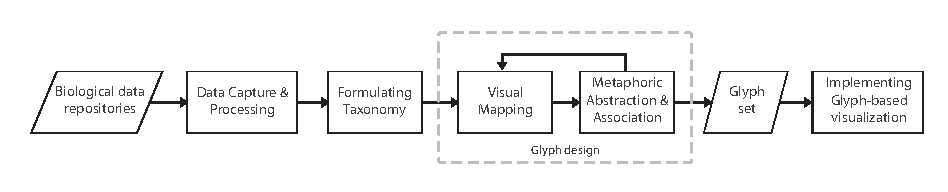
\includegraphics[scale=0.56]{images/glyph-taxonomy/workflow.eps}
\caption{A systematic process for creating glyph based representations.}
\label{fig:workflow}
\vspace{-10pt}
\end{figure}

\textbf{Data Capture and Processing}. We first retrieved workflow metadata from a biological repository (content of the ArrayExpress archive), through use of a multi-threaded harvesting operation. All experimental workflows were then converted using a MAGE-Tab to ISA-Tab converter, the latter format being more general than the former and can be used to carry metadata payloads for many types of experiments, making the data processing program more ``future-proof''.

From the 21,000 ISA-Tab files, we extracted all names of protocols (processes) and biological materials, chemical materials, devices and data used in annotation. We also computed the occurrence of each material and process found in the entire set of ISA-Tab files, which have been used as one of the metrics in the next stage (see Section 5 for details). This step results in 61 process names and 3492 names of inputs and outputs (e.g., biological and chemical materials, device measurements and data).

\textbf{Taxonomy Formulation}. Since a taxonomy for such a large collection of terms is absent, we, for starters, established a set of categorization schemes with the help of domain experts. For example, one of the schemes for categorizing processes may be based on different biological inputs to a process (e.g., molecule, cell, organism, etc.). Another scheme may be based on processing methods (e.g., perturbation, combination, etc.). We computed the quality measures of each scheme based a set of generic metrics (see Section \ref{sec:Taxonomy}) then created a taxonomic tree by recursively selecting the best categorization scheme based on the quality measures. We finalized the organization of the taxonomy by allowing domain experts (2 co-authors) to make adjustments according to domain-specific conventions. All leaf nodes of the resulting taxonomy tree are names extracted from the workflow metadata. All non-leaf nodes represent a categorization scheme.

\textbf{Glyph Design}. First, we established an ordering of commonly-used visual channels based on the literature focused on perception and visualization (see Section \ref{sec:Glyphs}). This allows us to systematically compare the order of categorization schemes in the taxonomy with the order of different visual channels. Ideally, schemes at the upper level of the tree can be mapped to visual channels which are more prominent to our visual system.

We then proceeded to the glyph design process involving two intertwined sub-processes for \textbf{visual mapping} and \textbf{metaphoric abstraction and association}. We proposed various options of visual channels for each categorization scheme featured in the taxonomic tree. We considered the merits of these visual channels and identify potential conflicts with the visual channels that have been assigned to other schemes. With the direct help from domain experts, we tried to identify a metaphoric abstraction
or association for each design option proposed. We evaluated and recorded the intuitiveness and suitability of the abstraction and metaphor association.

Informed by the results the two sub-processes, we finalized a glyph set by selecting a design option for each scheme, while maintaining the order of discriminative capacity of visual channels, minimizing conflicts between different channels, and maximizing the use of metaphoric abstraction and association.

\textbf{Implementation of Glyph-based Visualization}. We then integrated the glyph set with a layout algorithm to form a prototype system for workflow visualization (see Section \ref{sec:Workflow}). For demonstration purposes, we tested the workflow visualization in conjunction with ISAcreator, a popular domain agnostic biological experiment metadata capture tool.

% ==================
\section{Taxonomy Generation}
\label{sec:Taxonomy}

Given a large collection of concepts, we should ideally make use of a standard taxonomy, where non-leaf nodes represent different categorization schemes and each scheme provides subclasses that lead to different sub-trees. In many circumstances, however, there is no agreed taxonomic tree as establishing a standard categorization requires non-trivial scientific effort that often spans over a few decades.

The algorithm described below is not intended to establish a semantic-rich taxonomic tree for classifying concepts.
It is designed purely for addressing the needs for ordering various categorization schemes (when there is no such an agreed order) to aid glyph design, and for devising a useful tree data structure in implementing the mapping between concepts and glyphs in workflow visualization.

Hence, the criteria used for structuring the tree are based on usage of the concepts and the structural quality of the tree to be constructed.

Taxonomy is a long standing concept that can be traced back to 3000BC \cite{maguire12}. Automatic taxonomy generation has been an active field in computer science and computational biology with existing work largely focusing on clustering algorithms (e.g., \cite{krishnapuram03}). Many such algorithms assume the availability of similarity measures for ordering entities rather than relying on the existence of individual categorization schemes. In these algorithms, there is usually no attempt towards application of a metric for creating meaningful non-leaf nodes in the resulting tree. In this work, it is essential to keep each categorization scheme as a non-leaf node unless it is redundant.

\subsection{Ordering Classification Schemes}
\label{sec:Algorithm}

Let $\mathcal{X} = \{ x_{1}, x_{2}, \ldots, x_{n} \}$ be a set of concepts to be classified.
In our application, this is the set of all valid names of biological processes and IOs (inputs and outputs) in the database.
Each concept $x_i$ is associated with a scalar value, $\mu_i \in [0, 1]$, indicating its frequency of usage in relation to the total occurrence of all concepts in the database.
There are a number of categorization schemes, $\mathcal{S} = \{ S_1, S_2, \ldots, S_m \}$.
Each scheme, $S_k$ divides concepts into several classes, $c^k_1, c^k_2, \ldots, c^k_{l_k}$.
The relationship between the concept set $\mathcal{X}$ and different classification schemes can thus be represented by a Boolean matrix, $\mathbf{A}$, where each element $\alpha[i,j,k] = 1$ if concept $x_i$ belongs to the $j^{th}$ class of scheme $S_k$; otherwise $\alpha[i,j,k] = 0$.
In the context of feature-based categorization, one can also view each scheme $S_k$ as a feature, and each class under $S_k$ as a particular type of this feature.
Without losing generality, we assume that the classes under the same $S_k$ are disjoint.
It is also possible that a concept does not possess the $k^{th}$ feature, and hence does not belong to any class under $S_k$.

Given the above categorical information about the concept set $\mathcal{X}$, one can choose a categorization scheme $S_k \in \mathcal{S}$, which will divide $\mathcal{X}$ into a number of disjoint subsets corresponding to classes $c^k_1, c^k_2, \ldots, c^k_{l_k}$ and $c^k_0$.
The subset $c^k_0$ contains those concepts which $S_k$ is unable to classify.
The partitioning process can be repeated recursively by applying one of the remaining categorization schemes in $\mathcal{S}$ to each subset.
This results in a hierarchical categorization tree, which defines a taxonomy for the concepts set $\mathcal{X}$.

The ordering of the schemes in $\mathcal{S}$ thus determines the taxonomic structure of $\mathcal{X}$.
It is not difficult to anticipate that many criteria can be used to determine the ordering for a given concept set.
Some criteria will no doubt encode application-specific semantics, and some may be subjective or debatable.
However, there are also some common-sense criteria that are generic to most applications.
These include:

\textbf{Coverage}.
The number of concepts that can be classified by scheme $S_k$ is a capacity measure of $S_k$.
The more concepts that $S_k$ can classify (i.e., the fewer in $c^k_0$), the better.
The measure, which is normalized by the set size $\mid\!\mathcal{X}\!\!\mid=n$, can be defined as:

\begin{equation}
\label{eq:Coverage}
  M_1(S_k) = \frac{\sum_{i=1}^{n} \max_{1 \leq j \leq l_k} (\alpha_{i,j,k})}{n}.
\end {equation}

\textbf{Potential Usage}.
A categorization scheme that is higher up in the taxonomical tree is expected to be used more often in the application concerned.
The occurrence frequencies of concepts, $\mu_i$, enable us to estimate the potential usage of a classification scheme as follows:

\begin{equation}
\label{eq:Usage}
  M_2(S_k) = \frac{\sum_{i=1}^n \mu_i \max_{1 \leq j \leq l_k} (\alpha[i,j,k]) }
  {\sum_{i=1}^n \mu_i}.
\end {equation}

\textbf{Subtree Balance}.
Having a balanced node distribution in a tree is a desirable property of a tree structure.
It prevents a tree from having an excessive height, which corresponds to the need for more visual channels.
Let $l_k$ denote the number of subclasses in categorization scheme $S_k$,
$\tau_j$ be the number of concepts in each subclass $c^k_j, j=1, 2, \ldots, l_k$ and $\sigma_{\tau}$ and $\bar\tau$ be the standard deviation and mean respectively of $\tau_1, \ldots, \tau_{l_k}$.
We can measure the level of balance as follows:

\begin{equation}
\label{eq:Branch}
  M_3(S_k) = \begin{cases}
    0 & \sum_{i=1}^{l_{k}} \tau_{l_i} = 0 \\
    1 & \sigma_{\tau} < \epsilon (\epsilon \gt 0) \\
    P(\bar\tau \pm1 \mid N_{\bar\tau, \sigma_{\tau}}) & \bar\tau \gt 0 \; \& \;\sigma_{\tau} > \epsilon
  \end{cases}
\end {equation}

\noindent where $P$ is the probability that a value within $[\bar{\tau}-1, \bar{\tau}+1]$ falls under
the curve given by the normal distribution $N$ with $(\bar{\tau}, \sigma_\tau)$ \cite{patel96}.
There are two special cases.
When all values of $\tau_j$ are 0, $S_k$ cannot classify any concept; hence the metric returns a zero score.
When $\sigma_\tau = 0$, the subtree is totally balanced; hence the metric returns one.
As $\sigma_\tau$ approaches zero, the function $P$ becomes numerically unstable, we use a cut-off value $\epsilon$ to prevent this. In this work, we set $\epsilon = 0.00001$.
The normal distribution is preferred over a $\chi$-test, as $\chi$ may not be reliable when $l_k$ is a small number.

\textbf{Number of Subclasses}.
All visual channels used in glyphs have limited discriminative capacity.
A higher number of subclasses in a scheme would require visual encoding to have more codewords (e.g., more colors or more shape types), which will increase users' cognitive load in learning, remembering, and recognizing the codewords.
It is thus more desirable to have a smaller number of subclasses, except that a categorization scheme with fewer than 2 sub-classes is useless.
Let $\eta^{\top}$ be an up-limit for the number of codewords, which is set to 10 in this work.
We introduce the following metric to measure the discriminative capacity of a scheme:

\begin{equation}
\label{eq:Branch}
  M_4(S_k) = \begin{cases}
    0 & \eta_k < 2 \\
    \frac{\eta^{\top}-\eta_k+2}{\eta^{\top}} & 2 \leq \eta_k \leq \eta^{\top} \\
    \frac{1}{\eta^{\top}} & \eta_k > \eta^{\top}
  \end{cases}
\end {equation}

Although the above four metrics have been normalized to ensure their functional values within the $[0, 1]$ domain, the distribution of the values for different schemes can still be rather application-specific and may vary substantially between different metrics. This may lead to inconsistency in combining these metrics.

We thus provide an optional linearization filter for these metrics by mapping the values obtained using a each metric $M_i$ into fractional ranking numbers, which are then normalized into the $[0, 1]$ domain with 1 being the best and 0 the worst. For example, consider a set of six schemes with metric values:
%\[
%  (S_1, 0.5), (S_2, 0.3), (S_3, 0.5), (S_4, 0.8), (S_5, 0.8), (S_6, 0.6).
%\]
%
%\noindent We first sort the set and map the metric values to fractional ranking numbers as:
%\[
%  (S_4, 1.5), (S_5, 1.5), (S_6, 3), (S_1, 4.5), (S_3, 4.5), (S_2, 6).
%\]
%
\[
  (S_1, 0.5), (S_2, 0.3), (S_3, 0.54), (S_4, 0.8), (S_5, 0.85), (S_6, 0.6).
\]

\noindent We first sort the set:
\[
 (S_2, 0.3), (S_1, 0.5), (S_3, 0.54), (S_6, 0.6), (S_4, 0.8), (S_5, 0.85)
\]

\noindent We then obtain the normalized ranking values via the \emph{distance for ordinal variables} function $\sigma=\frac{r-1}{R-1}$ where R is the top rank and r is the rank position for each schema.
\[
  (S_2, 0), (S_1, \frac{1}{5}), (S_3, \frac{2}{5}), (S_6, \frac{3}{5}), (S_4, \frac{4}{5}), (S_5, \frac{5}{5}).
\]

We denote this filter as a function $R(S_k, M_i, \mathcal{S})$. Using the above set of metrics in conjunction with the filter $R$, we can derive a combined metric as
\[
  M(S_k) = \frac{\sum_1^4 \omega_t R(S_k, M_t(S_k), \mathcal{S})}{\sum_1^4 \omega_t}.
\]

\noindent where $\omega_t, t=1,2,3,4$ are user-adjustable weights for the four individual metrics. Similar to weights in clustering algorithms, these weights need to be used with care as they introduce additional semantics into the ordering algorithm. 

Equipped with the combined metric $M$, the algorithm for establishing an order of different schemes in $\mathcal{S}$ can be described as follows:

% TODO: Add this back in. 
%Rendering isn't completely right here... check with Min.
% \begin{program}
% \PROC select(\mathcal{S}, \mathcal{X}) \BODY
% S_{BEST} := null;  m_{BEST} := 0;
% \FOR S \in \mathcal{S} \DO
%      m := M(S);
%      \IF m > m_{BEST}
%           S_{BEST} := S;  m_{BEST} := m;
%           output(S_{BEST});
%           $remove $S_{BEST}$ from $\mathcal{S};
%           $split $\mathcal{X} $into subsets$ \mathcal{X}_{1}, \mathcal{X}_{2}, \ldots $, based on $S_{BEST};

%          \IF \mid subsets \mid \leq 1
%                return;
%         \FI
%         \FOR $each subset$ \mathcal{X}_{k} \DO
%             select(\mathcal{S}, \mathcal{X}_{i});
%        \OD
%    \FI
% \OD \ENDPROC
% \end{program}

% To illustrate our approach more clearly we present a more simple example related to classification of household items.

\subsection{Application to the Biological Case Study}
%
The biological community has built over the years a comprehensive collection of resources to archive experimental data. As molecular biology became a more data intensive field with the advent of DNA microarrays, came the need to store not only measurements but also ancillary annotation describing experimental conditions and set up, thus ensuring a metadata core always shipped with the data set. The sizes of microarray databases (GEO, AE) constitute prime resources for evaluating and testing our approach \cite{edgar02,parkinson11}. The content of ArrayExpress was therefore accessed obtaining data via parallel calls, converting 21000 experiments and associated experimental metadata to ISA-Tab\cite{rocca-serra10,sansone12}. This step provided a harmonized format in which to represent not just transcriptomic data, but also genomic, proteomic, metabolomic and other classical experiment types.

Given the data sets, the code analyzes the content of these directories to determine the processes and IOs which exist within the experiments, and the number of times they occur. The analysis revealed 61 processes (a small number resulting from the homogeneity of the database where analysis techniques are targeted primarily towards DNA microarrays) with 1,845,089 occurrences and 8,223 properties of the sample of which 3492 were deemed to be IOs with 486,353 occurrences.

Several distinct, empirical but meaningful, categorizations were devised encompassing a number of facets defining the properties of the experimental process, either in terms of its participants or in terms of key process properties. Classifications, based on features such as the nature of process participants, the granularity scale, the nature of experiments and common types a treatments applied in biological experiments were developed. Some classifications were somewhat informed by the overall assumptions ISA model relies upon, where nodes can be either material or data files and where edges are processes acting upon those nodes. Others resulted from applying a small number of axioms discovered through consultations with domain experts. There were 6 classification schemes in all with a total of 23 sub-classifications, these are detailed in figure \ref{fig:fitness-classification}. Table \ref{tab:input-fragment} shows a snapshot of the input file used in the classification algorithm.

\begin{table}[t]
\begin{center}
\caption{A fragment of the input document passed to the taxonomy generation algorithm. Schemes are grouped by common names preceding the semi-colon, e.g. \emph{S1:On Material} refers to schema 1 and \emph{On Material} is the classification.}
\vspace{1mm}
\scalebox{0.58}{

\begin{tabular}{l|ccc|c|ccc}
\textbf{Process Name} & \textbf{Occurrences} & \textbf{S1:Material} & \textbf{S1:Data} & \textbf{\ldots} & \textbf{S6:in vitro} & \textbf{S6:in vivo} & \textbf{S6:in silico}\\
\hline
\textit{labeling} & 390811 & 1 &  & \ldots & 1 &  &  \\
\textit{nucleic acid extr.} & 350267 & 1 &  & \ldots & 1 &  & \\
\textit{hybridization} & 345671 & 1 &  & \ldots & 1 &  &  \\
\textit{feature extr.} & 267044 &  & 1 & \ldots &  &  & 1 \\
\textit{bioassay data trans.} & 176347 &  & 1 & \ldots &  &  & 1 \\
\textit{grow} & 116194 & 1 &  & \ldots &  & 1 &  \\
\textit{pool} & 68004 & 1 &  & \ldots & 1 &  &  \\
\ldots & \ldots & \ldots & \ldots & \ldots & \ldots & \ldots & \ldots \\
\hline
\end{tabular}
}
\end{center}
\vspace{-5mm}
\label{tab:input-fragment}
\end{table}

The schemes are not tied to any existing taxonomic tree, may not be orthogonal and/or may be redundant with respect to others. The development of the classifications was not the result of application of any knowledge engineering methods and there is no ontological commitment, although in theory the classification names used could be derived from an ontological framework. The reason for not relying an ontology in the first place was risk mitigation, where use would almost certainly result in an unbalanced tree as occurrence counts for the terms would not be considered, resulting in creation of many glyphs that would never be used. 

\begin{figure}[ht!]
\centering
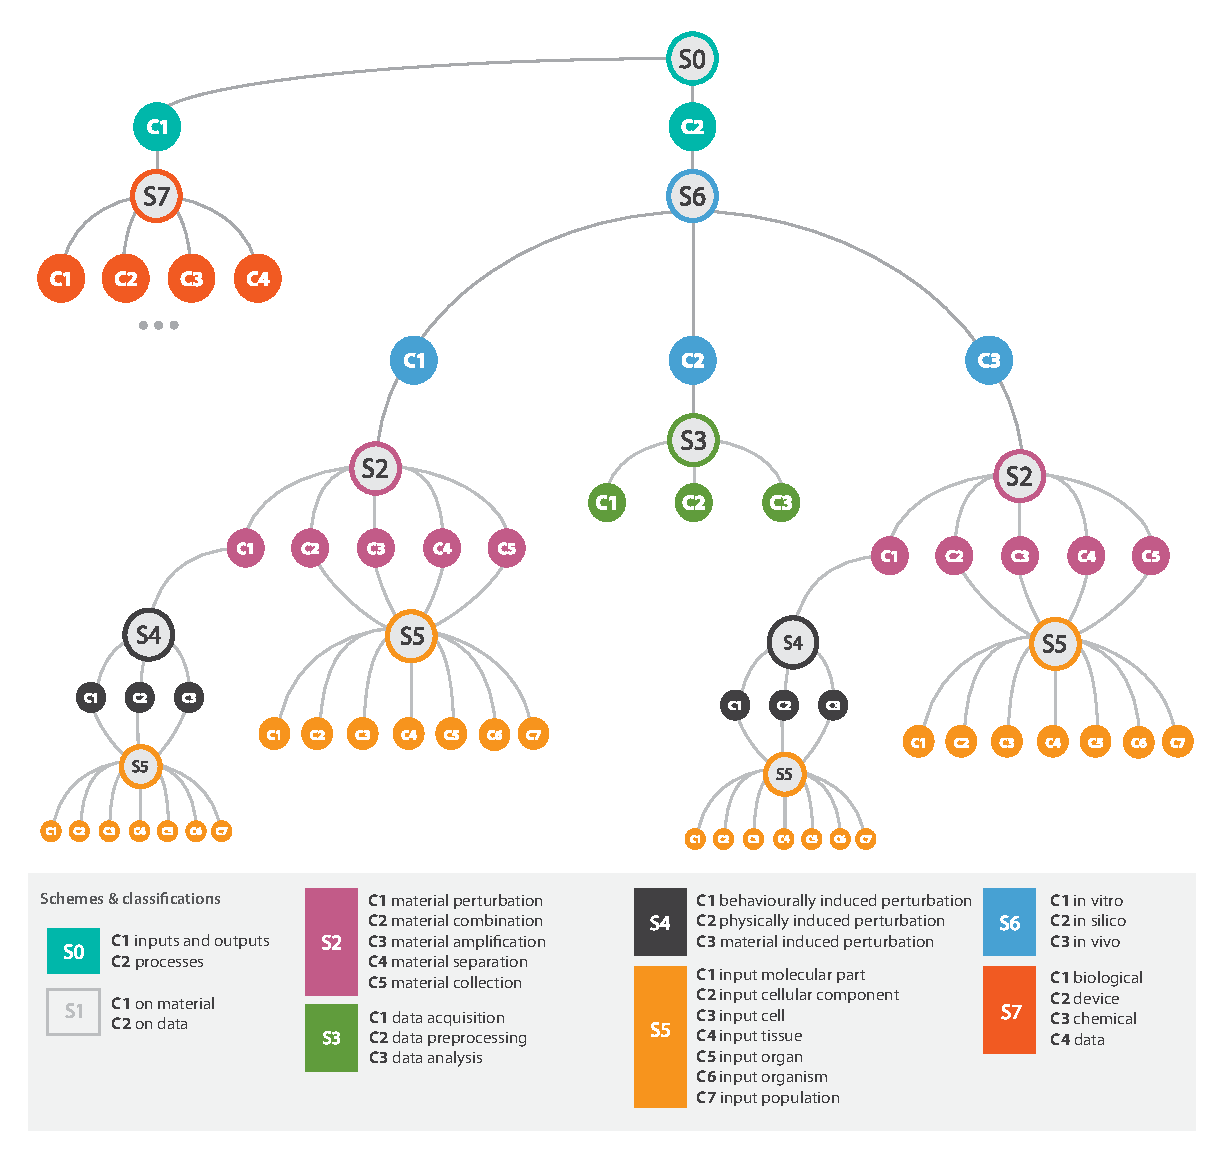
\includegraphics[scale=0.44]{images/glyph-taxonomy/fitness-classification.eps}
\caption{The classification algorithm arranged the classification schemes in the above order.}
\label{fig:fitness-classification}
\vspace{-10pt}
\end{figure}

The creation of the tree shown in Fig. \ref{fig:fitness-classification} was a largely iterative quest with continuous involvement of domain experts checking to ensure that the classifications assigned were meaningful. From early versions of the classification matrix creation, classifications were removed, added or merged in consultation with those who knew the data domain. For example, in \emph{S2} there were sub-classifications in \emph{Genetic Modification \& Labeling} which are types of \emph{Material Combination}. Therefore, these sub-classifications were removed since it would be technically and semantically incorrect to keep them. These early interactions emphasized the importance of having domain experts in the loop, otherwise classifications and subsequent glyphs would not be as well created as they could be.

The algorithm managed to correctly place the classifications where they were expected (checks were made by hand to ensure that the algorithm performed well). Schema \emph{S6} (\emph{in vitro}, \emph{in silico} and \emph{in vivo}) was the best top level classification due to its overall fitness metric of 3.08 with individual metrics found to be: M1 = 1.0; M2 = 1.0; M3 = 0.9; and M4 = 0.18. \emph{S6} was closely followed by \emph{S1} (on material and on data), however after the top level separation, \emph{S1} became redundant as a result of the top level implicitly making a split on data (in silico) and materials (in vitro and in vivo). The algorithm successfully detected this redundancy; hence $S1$ is absent from Fig. \ref{fig:fitness-classification}. 

Although the algorithm performed as expected, a possible criticism of the algorithm could be highlighted in the placement of \emph{S5} below \emph{S4}. \emph{S5} could have been placed above \emph{S4} in line with the observation that, for the majority of cases, \emph{S5} was selected over \emph{S4}. The reason \emph{S5} wasn't used to sub-classify C1 of \emph{S4} is due to its number of classifications (7) being greater than that of \emph{S4} (3), therefore \emph{S4} was selected primarily on this metric even though the sub-tree balance of \emph{S5} (0.8) was slightly better than that of \emph{S4} (0.68). To modify this behavior, it was necessary to involve domain experts in refining the tree based on their domain-specific knowledge and case-specific requirements.

% ---------------------------------------
\begin{table*}[!t]
\centering
\vspace{1mm}
\scalebox{0.67}{
\begin{tabular}{|l|l|l|l|l|l|l|c|l|c|}
\hline
 &  \textbf{Visual} & \multicolumn{ 4}{c|}{\textbf{Levels of Organization}} & \textbf{Popout} & \textbf{Hierarchy} & \textbf{Summary} & \textbf{Convention} \\
%
\textbf{Regions} & \textbf{Channels} & \textbf{Associative} & \textbf{Selective} & \textbf{Ordered} & \textbf{Quantitative} & \textbf{Effect} & \textbf{Effect} & \textbf{Strength} & \textbf{\& Metaphor} \\ \hline
%
a) Main & 1. Colour & Yes & Yes & Yes & 	& ***** & Strong  & ***** & application \\ \cline{ 2- 7}\cline{ 9- 9}
 & 2. Size &  & Yes & Yes & Yes 		& *** &   & **** &  specific \\ \cline{ 2- 7}\cline{ 9- 9}
 & 3. Shape & Yes & Yes &  &			& *** &   & *** &  \\ \cline{ 2- 7}\cline{ 9- 9}
 & 4. Orientation & Yes & Yes &  & 		& *** &   & *** & \\ \cline{ 2- 7}\cline{ 9- 9}
 & 5.Texture & Yes & Yes & Yes & 		& ** &    & ** &  \\ \cline{ 1- 9}
b) Supplementary & 6-10 (same as 1-5) &  &  &  &  &  & Medium &  & \\ \cline{ 2- 7}\cline{ 9- 9}
 & 11. Planar & Yes & Yes &  & Yes		& *** &  &  *** &  \\ \cline{ 1- 10}
c) Interior & Contains (a+b)) &  &  &  &  &				&  Low &  & \\ \hline
\end{tabular}
}
\caption{Perceptual strength of different visual channels based on levels of organization studied by Bertin\cite{Bertin:1983:book} and Green\cite{green98}, channel availability to pre-attentive processing (known as the ``popout'' effect) studied extensively in psychology \cite{williams67,duncan89,luck94,Bertin:1983:book,green98,wolfe89,treisman77,palmer77,parkhurst02}, and hierarchy effect studied by Navon \cite{navon77} and Love \cite{love99}.
The summary strength of each channel is estimated and it should be considered in conjunction with application-specific conventions and metaphors.}
\vspace{-5mm}
\label{tab:visual-variables}
\end{table*}



%\begin{table*}[t!]

\begin{center}
\scalebox{0.60}{
\begin{tabular}{|l|l|l|l|l|l|l|l|l|l|l|l|l|l|l|l|l|l|l|}
\hline
 &  & \multicolumn{ 5}{c|}{\textbf{\textit{Main}}} & \multicolumn{ 6}{c|}{\textbf{\textit{Supplementary}}} & \multicolumn{ 6}{c|}{\textbf{\textit{Interior}}} \\ \hline
 &  & \textbf{Colour} & \textbf{Size} & \textbf{Shape} & \textbf{Orientation} & \textbf{Texture} & \textbf{Colour} & \textbf{Size} & \textbf{Shape} & \textbf{Orientation} & \textbf{Texture} & \textbf{Planar} & \textbf{Colour} & \textbf{Size} & \textbf{Shape} & \textbf{Orientation} & \textbf{Texture} & \textbf{Planar} \\ \hline
\multicolumn{ 1}{|l|}{\textbf{\textit{Main}}} & \textbf{Colour} & \cellcolor{Gray} & $\gt$\cellcolor{Orange} \cite{williams67,luck94} & $\gt$\cellcolor{Orange} \cite{williams67} & $\gt$\cellcolor{Orange} \cite{luck94, parkhurst02} & Unk\cellcolor{Cream} & $\gt$\cellcolor{Orange} & $\gt$\cellcolor{Orange} & $\gt$\cellcolor{Orange} & $\gt$\cellcolor{Orange} & Unk\cellcolor{Cream} & Unk\cellcolor{Cream} & $\gt$\cellcolor{Orange} & $\gt$\cellcolor{Orange} & $\gt$\cellcolor{Orange} & $\gt$\cellcolor{Orange} & Unk\cellcolor{Cream} & Unk\cellcolor{Cream} \\ \cline{ 2- 19}
\multicolumn{ 1}{|l|}{} & \textbf{Size} & $\lt$\cellcolor{Blue} & \cellcolor{Gray} & $\gt$\cellcolor{Orange} \cite{williams67} & $\gt$\cellcolor{Orange} \cite{williams67,luck94} & Unk\cellcolor{Cream} & $\gt$\cellcolor{Orange} & $\gt$\cellcolor{Orange} & $\gt$\cellcolor{Orange} & $\gt$\cellcolor{Orange} & Unk\cellcolor{Cream} & Unk\cellcolor{Cream} & $\gt$\cellcolor{Orange} & $\gt$\cellcolor{Orange} & $\gt$\cellcolor{Orange} & $\gt$\cellcolor{Orange} & Unk\cellcolor{Cream} & Unk\cellcolor{Cream} \\ \cline{ 2- 19}
\multicolumn{ 1}{|l|}{} & \textbf{Shape} & $\lt$\cellcolor{Blue} & $\lt$\cellcolor{Blue} & \cellcolor{Gray} & $\gt$ \cite{luck94}\cellcolor{Orange} & Unk\cellcolor{Cream} & $\gt$\cellcolor{Orange} & $\gt$\cellcolor{Orange} & $\gt$\cellcolor{Orange} & $\gt$\cellcolor{Orange} & Unk\cellcolor{Cream} & Unk\cellcolor{Cream} & $\gt$\cellcolor{Orange} & $\gt$\cellcolor{Orange} & $\gt$\cellcolor{Orange} & $\gt$\cellcolor{Orange} & Unk\cellcolor{Cream} & Unk\cellcolor{Cream} \\ \cline{ 2- 19}
\multicolumn{ 1}{|l|}{} & \textbf{Orientation} & $\lt$\cellcolor{Blue} & $\lt$\cellcolor{Blue} & $\lt$\cellcolor{Blue} & \cellcolor{Gray} & Unk\cellcolor{Cream} & $\gt$\cellcolor{Orange} & $\gt$\cellcolor{Orange} & $\gt$\cellcolor{Orange} & $\gt$\cellcolor{Orange} & Unk\cellcolor{Cream} & Unk\cellcolor{Cream} & $\gt$\cellcolor{Orange} & $\gt$\cellcolor{Orange} & $\gt$\cellcolor{Orange} & $\gt$\cellcolor{Orange} & Unk\cellcolor{Cream} & Unk\cellcolor{Cream} \\ \cline{ 2- 19}
\multicolumn{ 1}{|l|}{} & \textbf{Texture} & Unk\cellcolor{Cream} & Unk\cellcolor{Cream} & Unk\cellcolor{Cream} & Unk\cellcolor{Cream} & \cellcolor{Gray} & Unk\cellcolor{Cream} & Unk\cellcolor{Cream} & Unk\cellcolor{Cream} & Unk\cellcolor{Cream} & $\gt$\cellcolor{Orange} & Unk\cellcolor{Cream} & Unk\cellcolor{Cream} & Unk\cellcolor{Cream} & Unk\cellcolor{Cream} & Unk\cellcolor{Cream} & $\gt$\cellcolor{Orange} & Unk\cellcolor{Cream} \\ \hline
\multicolumn{ 1}{|l|}{\textbf{\textit{Supplementary}}} & \textbf{Colour} & $\lt$\cellcolor{Blue} & $\lt$\cellcolor{Blue} & $\lt$\cellcolor{Blue} & $\lt$\cellcolor{Blue} & Unk\cellcolor{Cream} & \cellcolor{Gray} & $\gt$\cellcolor{Orange} & $\gt$\cellcolor{Orange} & $\gt$\cellcolor{Orange} & Unk\cellcolor{Cream} & Unk\cellcolor{Cream} & $\gt$\cellcolor{Orange} & $\gt$\cellcolor{Orange} & $\gt$\cellcolor{Orange} & $\gt$\cellcolor{Orange} & Unk\cellcolor{Cream} & Unk\cellcolor{Cream} \\ \cline{ 2- 19}
\multicolumn{ 1}{|l|}{} & \textbf{Size} & $\lt$\cellcolor{Blue} & $\lt$\cellcolor{Blue} & $\lt$\cellcolor{Blue} & $\lt$\cellcolor{Blue} & Unk\cellcolor{Cream} & $\lt$\cellcolor{Blue} & \cellcolor{Gray} & $\gt$\cellcolor{Orange} & $\gt$\cellcolor{Orange} & Unk\cellcolor{Cream} & Unk\cellcolor{Cream} & $\gt$\cellcolor{Orange} & $\gt$\cellcolor{Orange} & $\gt$\cellcolor{Orange} & $\gt$\cellcolor{Orange} & Unk\cellcolor{Cream} & Unk\cellcolor{Cream} \\ \cline{ 2- 19}
\multicolumn{ 1}{|l|}{} & \textbf{Shape} & $\lt$\cellcolor{Blue} & $\lt$\cellcolor{Blue} & $\lt$\cellcolor{Blue} & $\lt$\cellcolor{Blue} & Unk\cellcolor{Cream} & $\lt$\cellcolor{Blue} & $\lt$\cellcolor{Blue} & \cellcolor{Gray} & $\gt$\cellcolor{Orange} & Unk\cellcolor{Cream} & Unk\cellcolor{Cream} & $\gt$\cellcolor{Orange} & $\gt$\cellcolor{Orange} & $\gt$\cellcolor{Orange} & $\gt$\cellcolor{Orange} & Unk\cellcolor{Cream} & Unk\cellcolor{Cream} \\ \cline{ 2- 19}
\multicolumn{ 1}{|l|}{} & \textbf{Orientation} & $\lt$\cellcolor{Blue} & $\lt$\cellcolor{Blue} & $\lt$\cellcolor{Blue} & $\lt$\cellcolor{Blue} & Unk\cellcolor{Cream} & $\lt$\cellcolor{Blue} & $\lt$\cellcolor{Blue} & $\lt$\cellcolor{Blue} & \cellcolor{Gray} & Unk\cellcolor{Cream} & Unk\cellcolor{Cream} & $\gt$\cellcolor{Orange} & $\gt$\cellcolor{Orange} & $\gt$\cellcolor{Orange} & $\gt$\cellcolor{Orange} & Unk\cellcolor{Cream} & Unk\cellcolor{Cream} \\ \cline{ 2- 19}
\multicolumn{ 1}{|l|}{} & \textbf{Texture} & Unk\cellcolor{Cream} & Unk\cellcolor{Cream} & Unk\cellcolor{Cream} & Unk\cellcolor{Cream} & Unk\cellcolor{Cream} & Unk\cellcolor{Cream} & Unk\cellcolor{Cream} & Unk\cellcolor{Cream} & Unk\cellcolor{Cream} & \cellcolor{Gray} & Unk\cellcolor{Cream} & Unk\cellcolor{Cream} & Unk\cellcolor{Cream} & Unk\cellcolor{Cream} & Unk\cellcolor{Cream} & $\gt$\cellcolor{Orange} & Unk\cellcolor{Cream} \\ \cline{ 2- 19}
\multicolumn{ 1}{|l|}{} & \textbf{Planar} & Unk\cellcolor{Cream} & Unk\cellcolor{Cream} & Unk\cellcolor{Cream} & Unk\cellcolor{Cream} & Unk\cellcolor{Cream} & Unk\cellcolor{Cream} & Unk\cellcolor{Cream} & Unk\cellcolor{Cream} & Unk\cellcolor{Cream} & Unk\cellcolor{Cream} & \cellcolor{Gray} & Unk\cellcolor{Cream} & Unk\cellcolor{Cream} & Unk\cellcolor{Cream} & Unk\cellcolor{Cream} & Unk\cellcolor{Cream} & Unk\cellcolor{Cream} \\ \hline
\multicolumn{ 1}{|l|}{\textbf{\textit{Interior}}} & \textbf{Colour} & $\lt$\cellcolor{Blue} & $\lt$\cellcolor{Blue} & $\lt$\cellcolor{Blue} & $\lt$\cellcolor{Blue} & Unk\cellcolor{Cream} & $\lt$\cellcolor{Blue} & $\lt$\cellcolor{Blue} & $\lt$\cellcolor{Blue} & $\lt$\cellcolor{Blue} & Unk\cellcolor{Cream} & Unk\cellcolor{Cream} & \cellcolor{Gray} & $\gt$\cellcolor{Orange} & $\gt$\cellcolor{Orange} & $\gt$\cellcolor{Orange} & Unk\cellcolor{Cream} & Unk\cellcolor{Cream} \\ \cline{ 2- 19}
\multicolumn{ 1}{|l|}{} & \textbf{Size} & $\lt$\cellcolor{Blue} & $\lt$\cellcolor{Blue} & $\lt$\cellcolor{Blue} & $\lt$\cellcolor{Blue} & Unk\cellcolor{Cream} & $\lt$\cellcolor{Blue} & $\lt$\cellcolor{Blue} & $\lt$\cellcolor{Blue} & $\lt$\cellcolor{Blue} & Unk\cellcolor{Cream} & Unk\cellcolor{Cream} & $\lt$\cellcolor{Blue} & \cellcolor{Gray} & $\gt$\cellcolor{Orange} & $\gt$\cellcolor{Orange} & Unk\cellcolor{Cream} & Unk\cellcolor{Cream} \\ \cline{ 2- 19}
\multicolumn{ 1}{|l|}{} & \textbf{Shape} & $\lt$\cellcolor{Blue} & $\lt$\cellcolor{Blue} & $\lt$\cellcolor{Blue} & $\lt$\cellcolor{Blue} & Unk\cellcolor{Cream} & $\lt$\cellcolor{Blue} & $\lt$\cellcolor{Blue} & $\lt$\cellcolor{Blue} & $\lt$\cellcolor{Blue} & Unk\cellcolor{Cream} & Unk\cellcolor{Cream} & $\lt$\cellcolor{Blue} & $\lt$\cellcolor{Blue} & \cellcolor{Gray} & $\gt$\cellcolor{Orange} & Unk\cellcolor{Cream} & Unk\cellcolor{Cream} \\ \cline{ 2- 19}
\multicolumn{ 1}{|l|}{} & \textbf{Orientation} & $\lt$\cellcolor{Blue} & $\lt$\cellcolor{Blue} & $\lt$\cellcolor{Blue} & $\lt$\cellcolor{Blue} & Unk\cellcolor{Cream} & $\lt$\cellcolor{Blue} & $\lt$\cellcolor{Blue} & $\lt$\cellcolor{Blue} & $\lt$\cellcolor{Blue} & Unk\cellcolor{Cream} & Unk\cellcolor{Cream} & $\lt$\cellcolor{Blue} & $\lt$\cellcolor{Blue} & $\lt$\cellcolor{Blue} & \cellcolor{Gray} & Unk\cellcolor{Cream} & Unk\cellcolor{Cream} \\ \cline{ 2- 19}
\multicolumn{ 1}{|l|}{} & \textbf{Texture} & Unk\cellcolor{Cream} & Unk\cellcolor{Cream} & Unk\cellcolor{Cream} & Unk\cellcolor{Cream} & Unk\cellcolor{Cream} & Unk\cellcolor{Cream} & Unk\cellcolor{Cream} & Unk\cellcolor{Cream} & Unk\cellcolor{Cream} & $\lt$\cellcolor{Blue} & Unk\cellcolor{Cream} & Unk\cellcolor{Cream} & Unk\cellcolor{Cream} & Unk\cellcolor{Cream} & Unk\cellcolor{Cream} & \cellcolor{Gray} & Unk\cellcolor{Cream} \\ \cline{ 2- 19}
\multicolumn{ 1}{|l|}{} & \textbf{Planar} & Unk\cellcolor{Cream} & Unk\cellcolor{Cream} & Unk\cellcolor{Cream} & Unk\cellcolor{Cream} & Unk\cellcolor{Cream} & Unk\cellcolor{Cream} & Unk\cellcolor{Cream} & Unk\cellcolor{Cream} & Unk\cellcolor{Cream} & Unk\cellcolor{Cream} & Unk\cellcolor{Cream} & Unk\cellcolor{Cream} & Unk\cellcolor{Cream} & Unk\cellcolor{Cream} & Unk\cellcolor{Cream} & Unk\cellcolor{Cream} & \cellcolor{Gray} \\ \hline
\end{tabular}


}
\end{center}
\caption{Comparison of selected retinal variables available for the glyph design and their expected priority interactions based on review of effects presented in Table 1.
Unk. Unknown: no data documenting the interaction. > superiority/precedence , < inferiority/deference where row value are on the left of the operator and column value is the right term of the the operator.}
\label{tab:visual-variable-strength}
\end{table*}


% ==============
\section{Visual Encoding}
\label{sec:Glyphs}
\subsection{Perceptual Guidance}
%
A \emph{glyph} is a small visual object composed of a number of \emph{visual channels} which can be used independently as well as constructively to depict attributes of a data record.
Glyphs are of a type of visual signs that can make use of visual features of other types of signs, such as icons, indices and symbols.

Although there are several books on sign design (e.g., \cite{barker00,abdullah06}), they focus on signage in public space, and offer empirical guidance on a large number of issues including standardization, size, location, illumination and so on.
Many of these issues are not quite relevant to the need for visualizing the workflows of biological experiments. Here, we draw our design principles mainly from findings in perception, especially in the area of visual search \cite{spoehr82,quinlan03}.

While the extensive use of signs, icons and pictograms in everyday life reflects their usefulness and effectiveness, several perceptual studies also directly or indirectly confirmed their perceptual and cognitive merits.
For example, Franks and Bransford's study on transformation of prototypes \cite{franks71} suggested that humans can learn to recognize glyphs by rules consciously as well as unconsciously.
The presence of iconic memory \cite{sperling60} may facilitate rapid comparison between glyphs in the same display, whereas it is less so for texts.

\textbf{Guideline on Semantic Relevance}.
Bertin \cite{bertin83} classified visual channels (which he referred to as retinal variables) into two categories, planar (location) and retinal (size, color, shape, orientation, texture and brightness).
Bertin proposed four semantic criteria for determining the suitability of different channels in representing certain types of information.
These semantic criteria are: \emph{associative}, \emph{selective}, \emph{ordered} and \emph{quantitative}.
These criteria are important guidelines, though there has been disagreement in the literature as to how individual visual channels are judged.
For example, Bertin considered shape as a non-selective variable.
Research has shown that shapes such as filled rectangles, circles and triangles do not allow the human visual system to identify one shape from another effectively in a rapid action when they form some global structures \cite{love99, navon77}, (they have poor ``pop-out'' effect).
However, the omission of all shapes as a selective visual channel has been challenged, for example, by \cite{treisman88,wang94,green98}, who show practice and familiarity can support selectivity with almost any shape.

\textbf{Guideline on Channel Composition}.
As a glyph is likely to feature a number of visual channels, the constructive composition may affect how individual channels are perceived.
A rich collection of literature on integral and separable dimensions shows that the combined dissimilarity of closely integrated visual channels exhibits Euclidean distance $\sqrt{d^2_a + d^2_b}$ \cite{krantz75,handelt72}, whereas that of separable visual channels exhibits city-block distance $d_a  + d_b$ \cite{burns78,shepard64}. 
The latter is more cost-effective than the former in rule-based encoding of multi-faceted concepts, therefore effective glyph design should encompass a non-conflicting set of separable retinal variables. 

\textbf{Guideline on Pop-out Effects}.
Many classic studies in perception also established the ``power'' of different visual channels in terms of \emph{pop-out effect} (pre-attentive search), and fixation (during attentive search)\cite{healey11}.
The \emph{pop-out effect} is one which allows identification of a target within a few nanoseconds of initial exposure to the visual search space.
A result of several milestone studies focusing on observed response times, the ordering of the four commonly used visual channels follows the consensus: color $\prec$ size $\prec$ shape $\prec$ orientation (e.g.,\cite{williams67,quinlan97,ropinski11}).
The symbol $\prec$ reads as \emph{precedes}. However, the strength of color over the other three channels is generally much more noticeable. 

\textbf{Guideline on Visual Hierarchy}.
%
\emph{Visual hierarchy}, with which the environment and objects around us are arranged is a well documented theoretical framework \cite{palmer77,navon77, love99, kinchla79,bar04}.
However, the literature contains a debate over the ways in which the visual system traverses this hierarchy.
There are four possible ways:
top-down (also called global processing) \cite{navon77};
bottom-up (also called local processing);
middle-out \cite{kinchla79};
and salient features (\emph{e.g., edges, points, colors}) \cite{rumelhart70}.
Because glyphs are relatively small in comparison with a whole visualization, we consider at such a ``localized level'', the top-down and salient features may play more significant roles.
The top-down assumption suggests that when consider a glyph in isolation, its global feature will affect visual search more than its local features.
Salient features are partly addressed by the pop-out effects.

\begin{figure}[t]
\centering
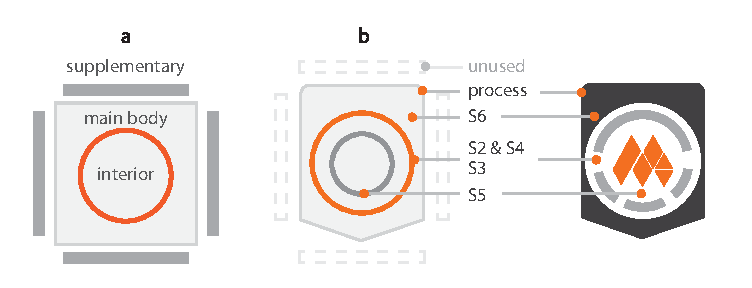
\includegraphics[width=86mm]{images/glyph-taxonomy/glyph-space.eps}
\caption{(a) The glyph template with a main body, an interior region and an exterior region (consisting of 4 sections).
(b) Our final design makes use of the main body and interior region.
The exterior is reserved for future extension.
% As we proceed to lower levels, size will have an impact on visual power\cite{duncan89}.
}
\label{fig:glyph-design}
\vspace{-10pt}
\end{figure}

Based on the above-mentioned perceptual guidance, we considered a generic glyph design template for this work as shown in Fig. \ref{fig:glyph-design}(a).
The template divides a glyph into three regions, namely \emph{main body}, \emph{exterior} and \emph{interior}.
In practice, each region can be divided into 2 or more sub-regions (e.g., a twin body glyph or 4 exterior sections), it is convenient to consider the three regions in abstraction.
The separation of these regions facilitates the basic separation of visual channels based on the composition guideline, while allowing us to consider them individually according to the hierarchy guideline.

In theory, the exterior and interior regions may also be divided into sub-regions in a recursive fashion though in practice this is tightly constrained or discouraged by the very limited display resolution typically available for glyphs.
Similar to the design convention for icons, pictograms are normally featured in the interior region.
The exterior region may be further divided in four sections (top, bottom, left and right).
If glyphs will be connected to form a network or graph (as in this work), the use of these four sections has to take into account the possible incoming and outgoing connections.

Table \ref{tab:visual-variables} summarizes relative merits of some of the most commonly-used visual channels in different regions according to Bertin's categorization, pop-out effects and hierarchy effects.
We estimated the overall discriminating capacity of each channel by using a summary rating in the penultimate column.
We also recognized the importance of the conventions and metaphors in an application.
We will discuss visual metaphors further in Section \ref{sec:Mapping}.
We added the last column to highlight the necessity to consider these in a design process.

It is difficult to establish an accurate ranking order of different visual channels by taking all perceptual effects into account in a quantitative manner.
The state of the art in perception research is yet to provide all evidence needed for a full and conclusive analysis.
Nevertheless, Table \ref{tab:visual-variables} can serve a qualitative guidance to glyph designs in this work, providing an ordering of visual channels in parallel with the ordering of categorization schemes discussed in Section \ref{sec:Taxonomy}.

% ---------------------------------------------------------
\subsection{Mapping Taxonomy to Visual Channels}
\label{sec:Mapping}

For each scheme in the taxonomic tree as shown in Fig. \ref{fig:fitness-classification}, we propose a number of design options.
Fig. \ref{fig:design-options} shows some examples of the proposed designs.
For example, the first column shows the use of colors to encode the classes of a categorization scheme.
The second column shows the use abstract shapes.
Some options convey an abstraction from pictorial representations of classes, and in other cases, we try to establish a metaphoric association between a visual channel and a biological categorization. 

Metaphoric visual representations enable domain-specific encoding using ``natural mapping'' \cite{siirtola05,norman02}. This natural mapping can make it easier for users to infer meaning from the glyph with less effort required to learn and remember them \cite{McDougall00}.
A recent study showed that visual metaphors can aid memorization of the information depicted in a visualization \cite{Borgo12}. However, the same study also showed that visually realistic metaphors 
(those with a lot of detail) may have a negative impact on performance in visual search. Moreover, realistic visual metaphors require a higher pixel resolution, and would lose their discriminating capacity in low resolution conditions. 

\begin{figure}[t!]
\centering
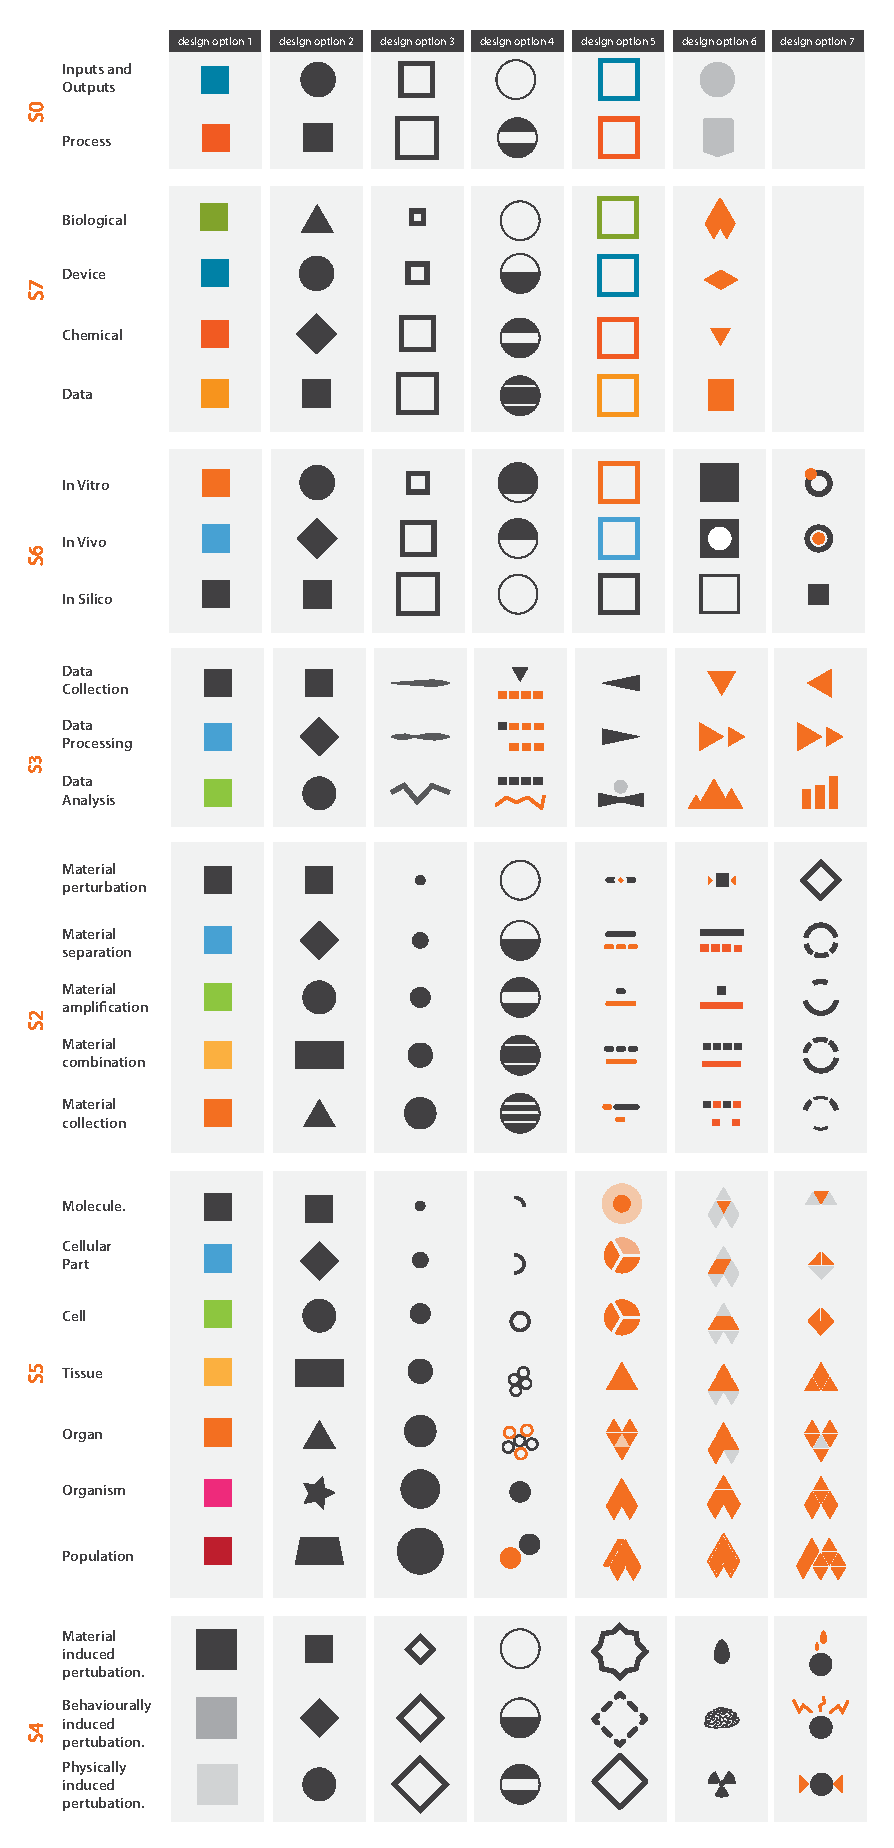
\includegraphics[scale=0.605]{images/glyph-taxonomy/design-options.eps}
\caption{Experimenting with visual channels: an overview of the various design options available for use in representing the different classifications. Most schemes for IO categorization are not shown due to space restriction.}
\label{fig:design-options}
\vspace{-10pt}
\end{figure}

Based on the design options shown in Fig. \ref{fig:design-options}, we followed the taxonomic tree in Fig. \ref{fig:fitness-classification} and identified the best option for each scheme in a hierarchical manner.
The evaluation criteria include:
%
\begin{itemize}
\vspace{-1mm}
\item
the discriminating capacities of different channels (Table \ref{tab:visual-variables});
\vspace{-2mm}
\item
metaphoric capacity for aiding learning and remembering;
\vspace{-2mm}
\item
potential conflicts, including spatial, perceptual and metaphoric conflicts, with visual channels that have already been assigned to other schemes in the tree;
\vspace{-2mm}
\item
encoding costs in terms of requirement for pixel resolution.
\end{itemize}

This process normally takes a few iterations, during which new design options and new metaphoric abstractions and associations are sometimes proposed.

\begin{figure}[t!]
\centering
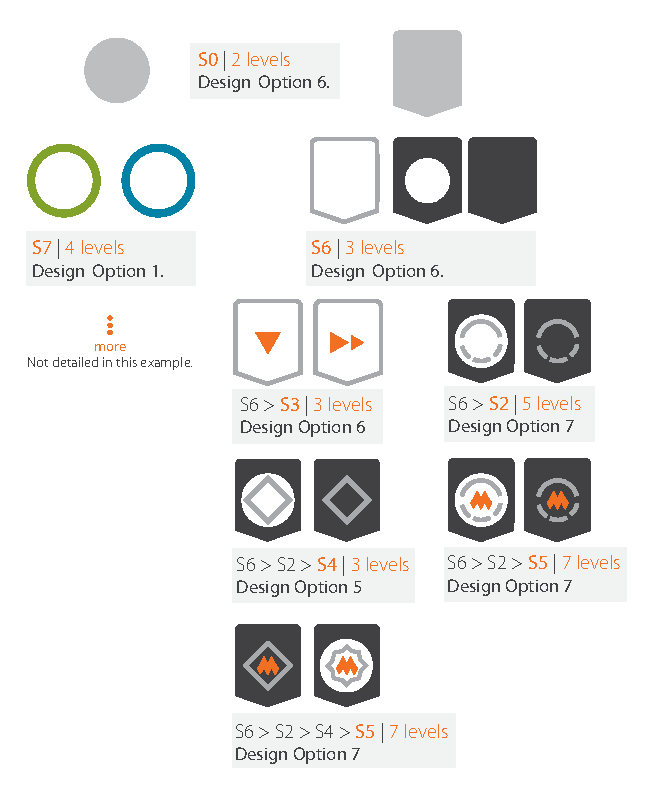
\includegraphics[scale=0.7]{images/glyph-taxonomy/glyph-design-selection.eps}
\caption{Formation of the final glyph design. Top level items require the greatest visual power. It is important to be able to distinguish each of the processes based on their parent level in the taxonomy. Distinguishable global shapes provide the difference between IOs (circles) and processes (squares with pointed bottom to indicate directionality).}
\label{fig:glyph-design-selection}
\vspace{-10pt}
\end{figure}

Based on the hierarchy in Fig. \ref{fig:fitness-classification}, we considered to use color and shape options for S0 (IOs vs. processes) and S7 (four classes of IOs).
As introducing 4 main body shapes to encode IOs is not an effective mapping for learning and remembering, we decided to assign outline color of the main body to encode S7, and use two basic shapes, circle and pentagon (a rectangle with a pointer to show workflow direction) to encode S0.
Since the main body or the pentagon will only be colored in black or white, S0 also implicitly encoded in using color symbolism, that is, color for IOs and black/white for processes.
In effect, S0 is encoded using two visual channels.
This redundancy can serve as an error detection in visualization \cite{Chen10}.

Fig. \ref{fig:glyph-design-selection} shows each of the five schemes for the process subtree, and the design option chosen from Fig. \ref{fig:design-options}.
Below we discuss our reasoning for selecting each of the design options for each scheme in the taxonomy.


\textbf{S6: Process environment}.
The taxonomic tree suggested a high priority for visual mapping, which is consistent with the domain experts' intuition.
We took advantage that black color was not used by S7 for IOs, we assigned a white background to \emph{in silico/in computer} (related to computational processes), and black to \emph{in vivo/in living)}  and \emph{in vitro/in glass} (related to materials).
Further more, we made use of a shape-based metaphor, fully-filled background for \emph{in vivo} (whole organism), and black background with white cut out for \emph{in vitro} (component of an organism).
Together, this was given in Fig. \ref{fig:design-options} as design option 6.
We maintained the overall appearance of the main body of process glyphs in black and white to avoid potential clash with material glyphs.

\textbf{S2: Types of Material Manipulation}.
S2 has 5 classes, and we adopted design option 7, which employs visual metaphors that encapsulate strong domain-specific meanings.
For example, visual symbol for the \emph{material amplification} class depicts a small segment becoming a large segment.

\textbf{S4: Type of Experimental Perturbation}.
S4 defines 3 further sub-classes of the \emph{material perturbation} class of S2.
Due to the low number of subclasses, we made use of line styles to modify the diamond shape of the \emph{material perturbation}.
We made metaphoric association of three line styles as:
``solid'' line for physically induced perturbation;
dash line, a common metaphor for uncertainty and unpredictability, for behaviorally induced perturbation; and
wavy line, which is closer to a circle (a visual signature for IOs), for material induced perturbation.

\textbf{S5: Levels of Material Granularity}.
This scheme has 7 subclasses (molecule, cellular part, cell, tissue, organ, organism and population), and finding a suitable visual channel was not straightforward. A simplest approach would be to use colors to fill the interior of the glyph, or to use some shape-based encoding.
After consulting the domain experts, these two options were ruled out.
In fact, domain experts preferred some pictograms to represent the 7 subclasses.
After considering a number of more realistic drawings, we found that it was not easy to create realistic representations that can differentiate all subclasses (e.g., cellular part vs. cell; organ vs. organism).
We designed a special set of icons as shown in Fig. \ref{fig:s5-metaphor} with three visual channels to aid learning, memorization and recognition.
The first visual channel is the overall shape and orientation.
The second visual channel is metaphoric abstraction and association.
For example, the shape of cell part indicates a portion of a cell.
Tissue is associated with a patch, organ with an abstract heart shape, organism with an abstract human, population with two abstract humans.
The third visual channel is the number of orange sub-shapes, representing the levels 1-7.
\begin{figure}[t!]
\centering
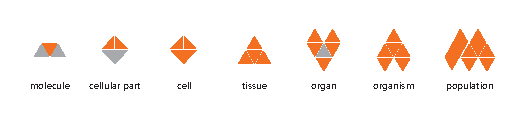
\includegraphics[scale=1]{images/glyph-taxonomy/s5-metaphor.eps}
\caption{Visual representations of the 7 classes in \emph{S5}.}
\label{fig:s5-metaphor}
\vspace{-10pt}
\end{figure}

\textbf{S3: Types of Data Manipulation}.
S3 defines a 3 further sub-classes of the \emph{in silico} class of S6.
We use three abstract pictograms to represent data capture, processing and analysis. The encoding makes use of the difference in overall shape, orientation, and number of triangles to aid learning, memorization and recognition. Note that these shapes will not be confused with those for S5 as the white background of the main body provides a distinct context of computing rather than IOs.

\begin{figure*}[t!]
\centering
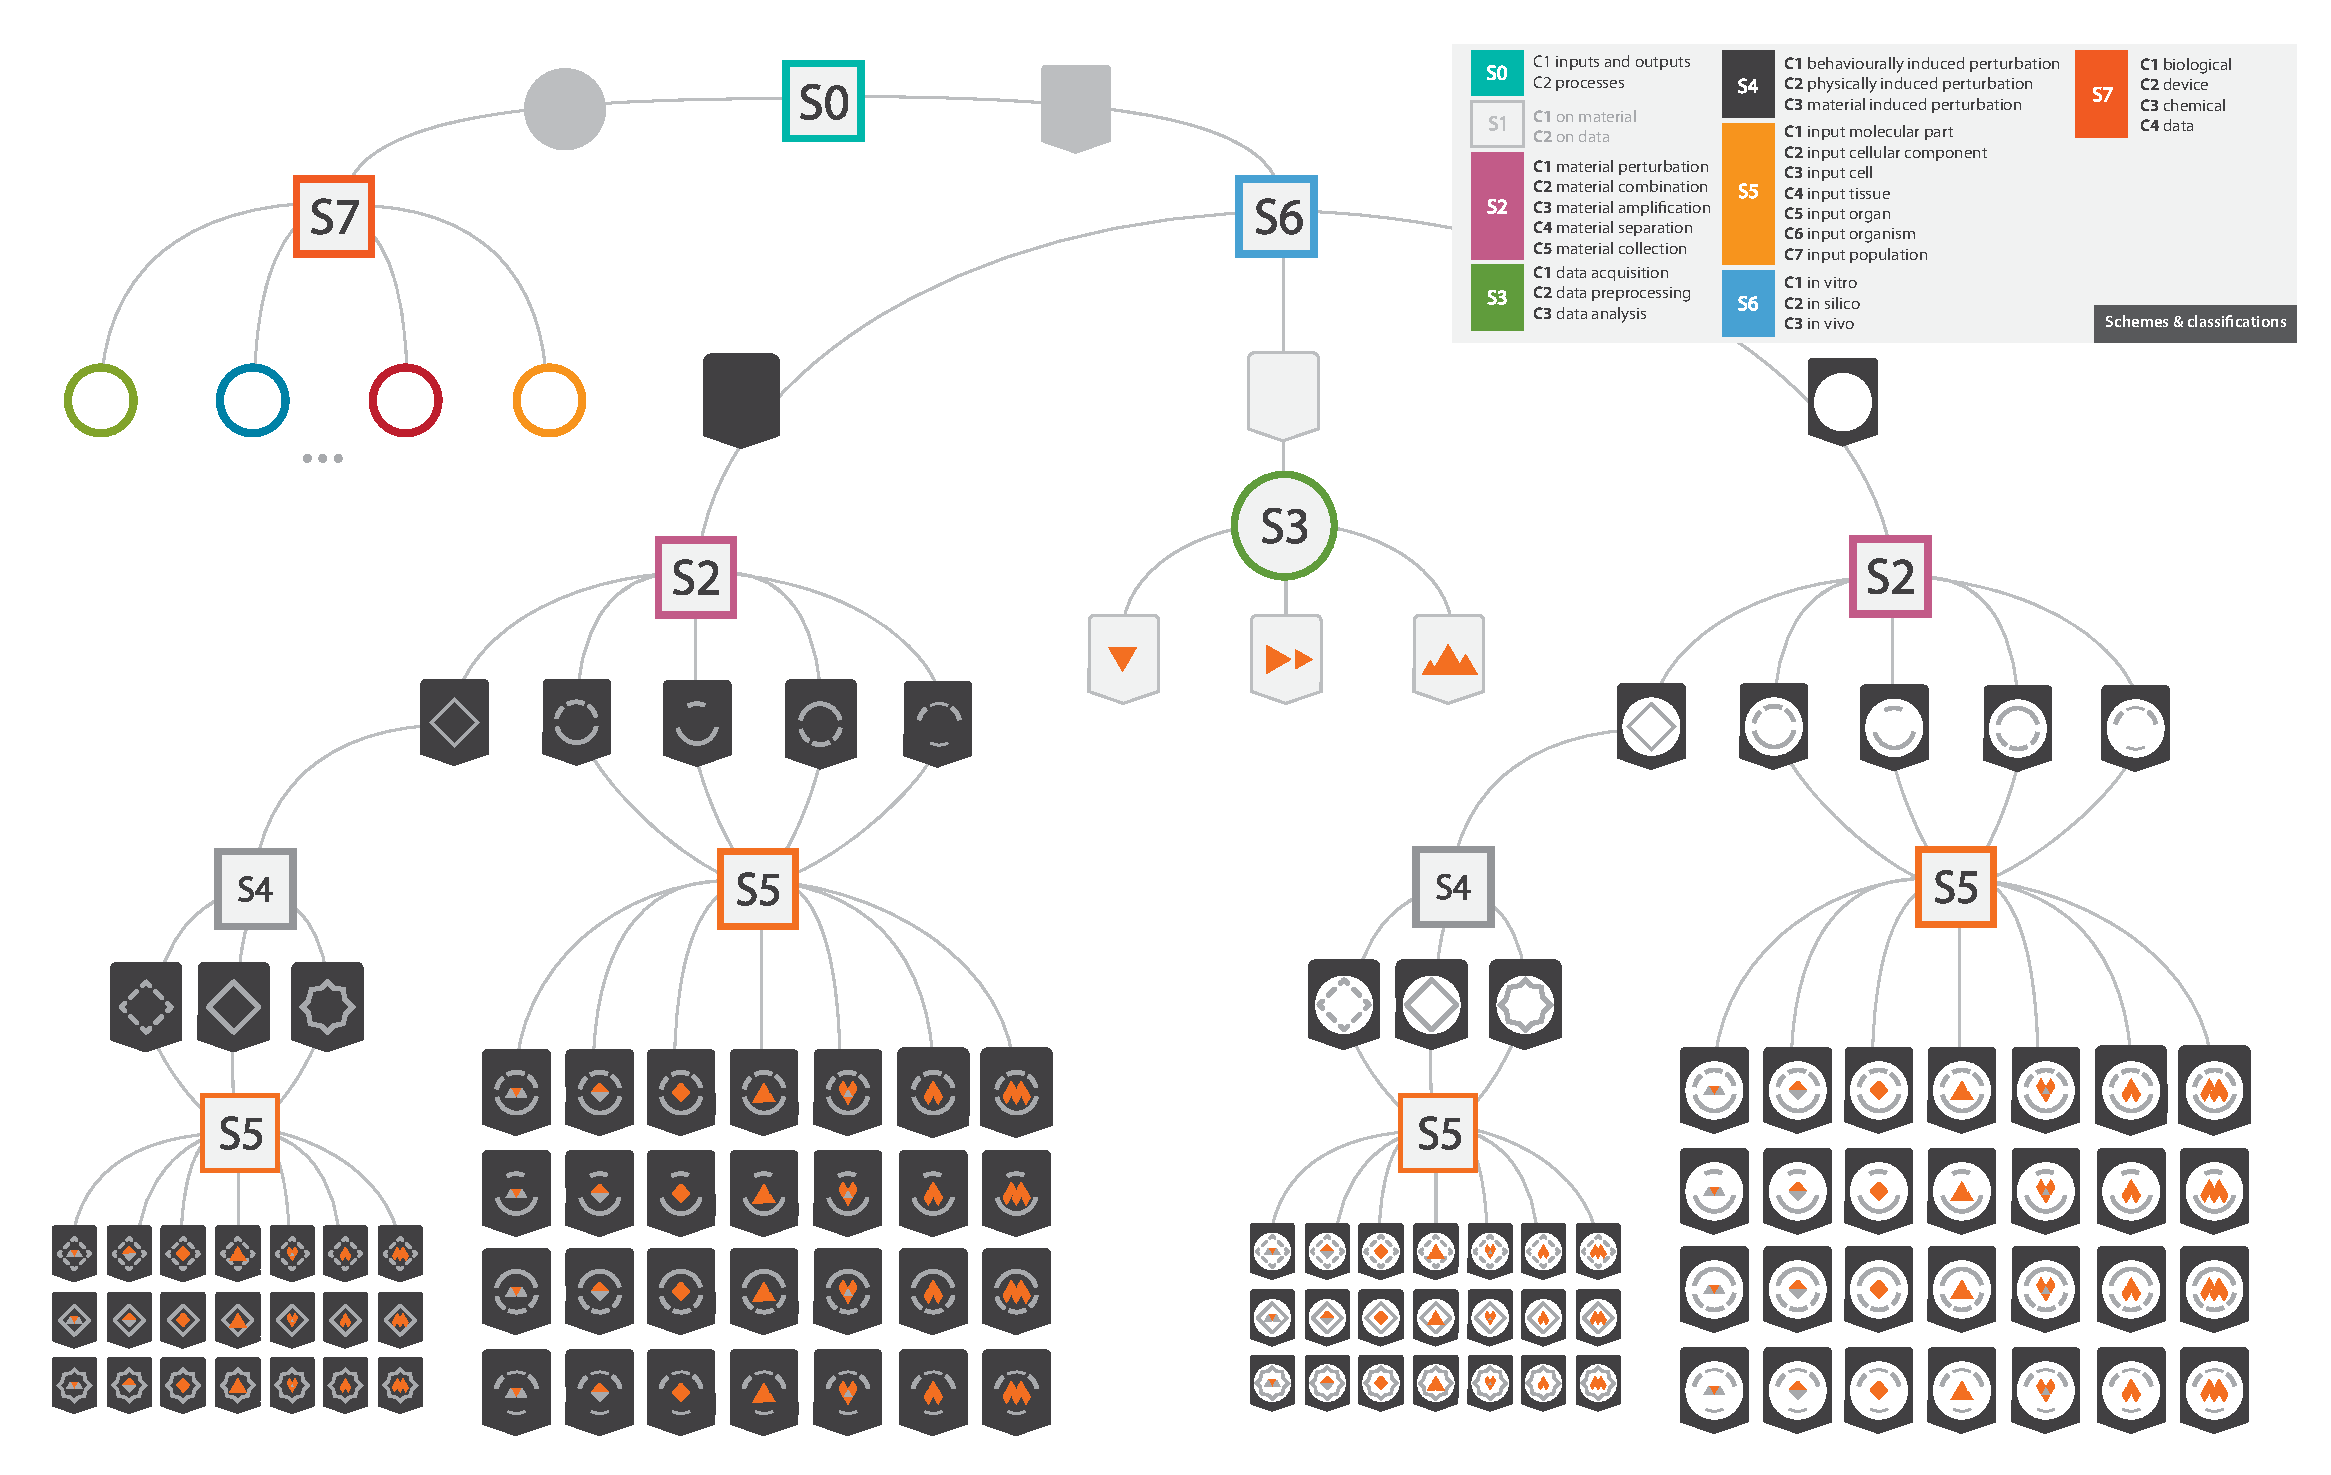
\includegraphics[scale=0.465]{images/glyph-taxonomy/full-tree.eps}
\caption{Overview of the taxonomy based glyph designs in the context of biodomain.}
\label{fig:full-tree}
\vspace{-5pt}
\end{figure*}

Following mapping of all schemes to design options, creation of all glyphs is a straightforward process.
Fig. \ref{fig:full-tree} shows all variations of the glyphs associated with the process sub-tree.

We introduced a ``crush'' test for the designed glyphs by scaling it to different pixel resolutions.
Fig. \ref{fig:crash-test} shows some example glyphs display at varying resolutions.
One can comfortably see all details at the 40$\times$40 level.
At the 10$\times$10 level, one can observe the visual signature of \emph{in vivo} and \emph{in vitro}.
Even at the lowest level (5$\times$5), one can still differentiate the two glyphs. 

\begin{figure}[t!]
\centering
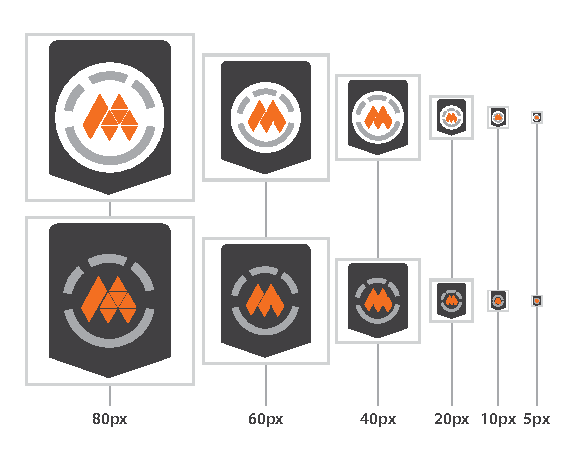
\includegraphics[scale=1]{images/glyph-taxonomy/crash-test.eps}
\caption{A ``crush'' test of glyphs to evaluate the discriminating capacity of various visual channels at different resolutions.}
\label{fig:crash-test}
\vspace{-5pt}
\end{figure}

% ===============
\section{Workflow Visualization and ISA Integration}
\label{sec:Workflow}

In order to visualize workflows of biological experiments, we had to address the following technical issues:
1) mapping from a name in the metadata to a glyph;
2) creating a workflow visualization with both node placement and connection display;
3) developing a prototype tool for a practical environment such as the ISA tools framework.

The mapping from concept name is achieved by a look-up table which is built from the matrix used in formulating the taxonomic tree and implemented as a tab delimited file.
Each concept name is mapped to a text tag encoding the traversal path from the root of the tree to the leaf node corresponding to the name.
The tag includes identifiers of the schemes and classes encountered.
With the path, a glyph can be constructed dynamically from the pre-defined visual mapping as described in the previous section.
The look-up table also enables storage of pre-rendered glyphs in an image format.

To generate the workflow, we made use of the layout algorithm available within the Prefuse visualization framework \cite{heer05}. This framework also brings with it functionality such as panning, zooming and filtering which bring more interactivity to the user and making navigation through large collections of workflows easier. The only requirement for use of Prefuse was a minimal amount of Java code to create the user interface coupled with creation of an XML file format native to Prefuse for representation of the tree structure. This XML format is configurable, we have configured it to contain: \emph{node type} (e.g., process), \emph{node
name} (e.g., labeling) and an image to be rendered, which is assigned using a look-up operation through the above mentioned tab delimited mapping file. The order of the XML elements within this file has direct implications on the order these elements are displayed in. Within the ISA-Tab format, there is an implicit time element found in the ordering of the columns in the study sample and assay files. This can be used to construct the XML elements through near direct mappings of processes and IOs, a workflow which is illustrated in Fig. \ref{fig:generating-workflow-from-text}. Recognizing branching events is an important part of workflow visualization as illustrated in \ref{fig:generating-workflow-from-text}. In software, these branch events can be identified when the preceding nodes of a process have the same names while the succeeding output nodes are different. Fig. \ref{fig:generating-workflow-from-text} highlights one such case, where branching occurs after extraction of 3 materials from one sample. 

Our software reads text-based ISA-Tab files as illustrated to create the XML notations required by Prefuse for rendering the experiment workflow illustrated in Fig. \ref{fig:teaser}(b).

\begin{figure}[t!]
\centering
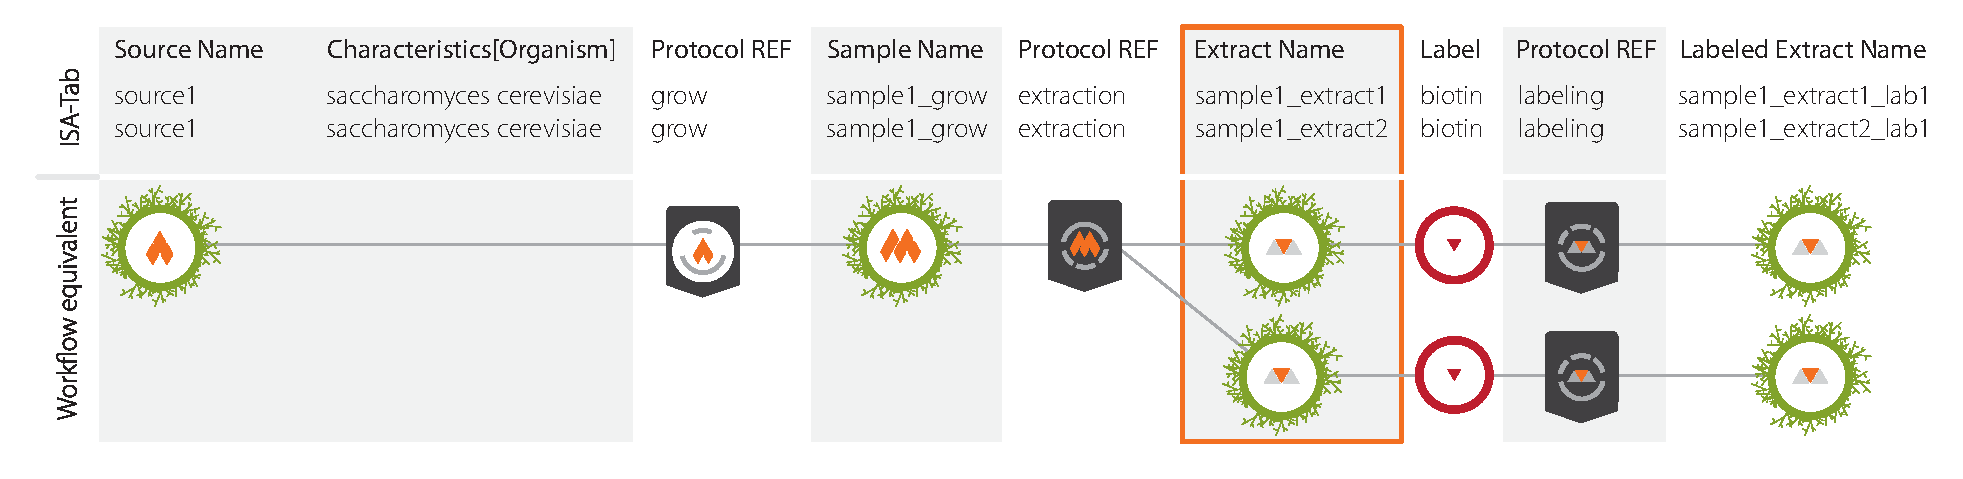
\includegraphics[scale=.2745]{images/glyph-taxonomy/generating-workflow-from-text.eps}
\caption{A workflow is recorded in text form within the ISA-Tab format.
Our software translates it to glyph-based visualization.
A branching event is automatically detected during the translation.}
\label{fig:generating-workflow-from-text}
\vspace{-10pt}
\end{figure}

\begin{figure}[ht!]
\centering
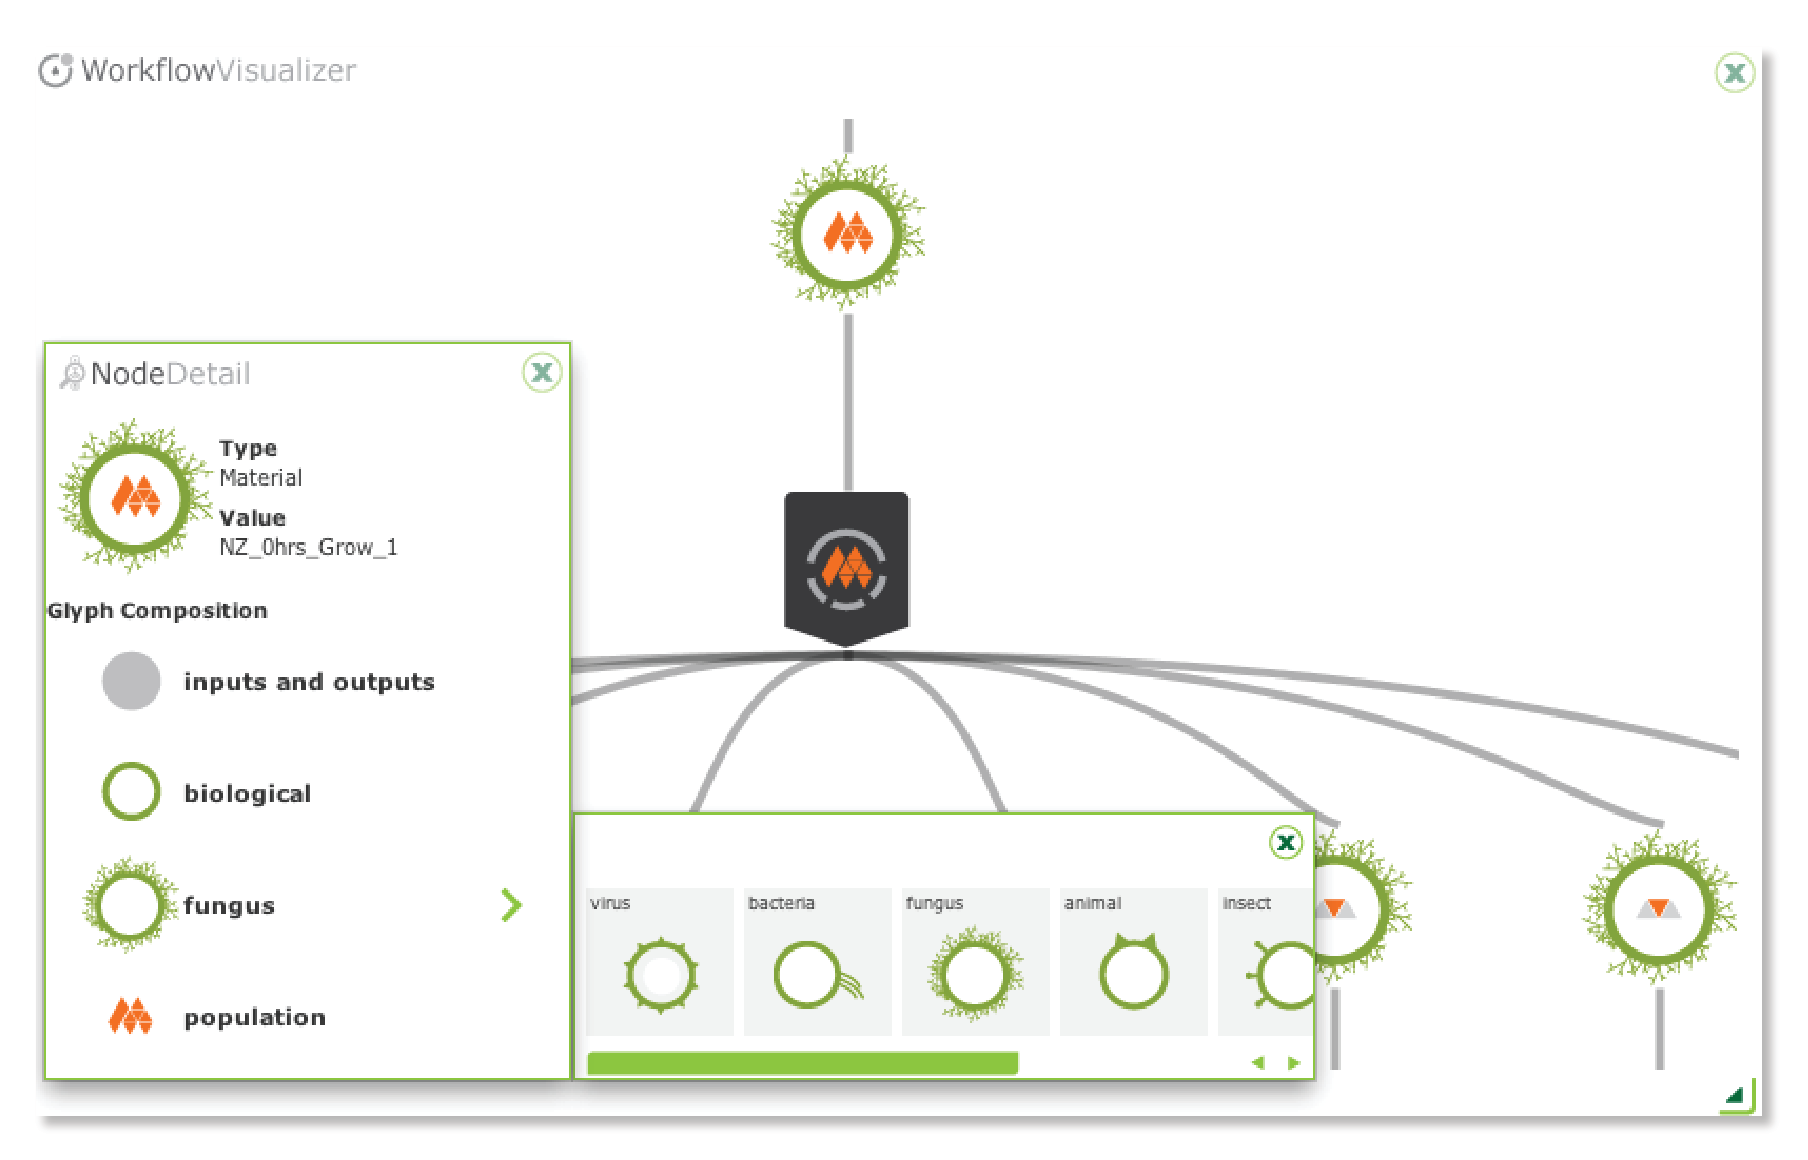
\includegraphics[scale=.295]{images/glyph-taxonomy/bio-workflow-example.eps}
\caption{User can interact with a workflow to view the text descriptions of individual glyphs in pop-up windows, which are also dynamic legends showing how the concept is categorized and how the corresponding glyph is decomposed into different elementary visual representations. Users can also use such a legend to find out other classes in a categorization scheme.}
\label{fig:bioworkflow-example}
\vspace{-15pt}
\end{figure}

The software is implemented as a Java application capable of processing ISA-Tab files to create experimental workflows using glyphs. For the purposes of broad dissemination in the near future, we have integrated the workflow visualization directly inside ISAcreator, a Java desktop application for creating and editing ISA-Tab files. Furthermore, the standalone workflow visualization shown in figures \ref{fig:bioworkflow-example}a and b makes use of the same ISA-Tab parser as available within ISAcreator. The integration involved the development of user interface elements for ISAcreator software to access the workflow visualization.
From the spreadsheet view, users may highlight rows (assays), right click and select an option named ``View workflow for assays'' to visualize the entire processing pipeline for the corresponding samples as shown in Fig. \ref{fig:teaser}(b).

\section{Conclusions and Future Work}
\label{sec:Conclusion}

Although it was established in psychology that people can learn rules of glyph encoding consciously as well as unconsciously \cite{franks71}, we do not expect users to learn and remember these glyphs without help. We thus allow users to find detailed text descriptions in pop-up windows interactively. As shown in Fig. \ref{fig:bioworkflow-example}, not only do these windows provide names of processes and IOs, they also serve as dynamic legends, showing how each glyph is decomposed into different elements corresponding to categorization schemes. One can also select a component to view all classes in a scheme.   

In this manuscript, we presented a systematic approach for glyph
design by using taxonomy as a guide. We demonstrated our approach by analyzing the content of a biological database and showed how our tree-building algorithm
could be used to take a large collection of concepts and generate a taxonomic tree, which
provides an ordering of a set of categorization schemes (i.e., attribute dimensions).
This enabled us to draw a parallel between the ordering of attribute dimensions with the ordering of visual channels compiled from the perception and visualization literature. 
We involved domain experts in refining the tree as well as in creating metaphoric abstraction and association for glyphs.
This work was followed by development of a prototype tool for glyph-based visualization of experimental design workflows as found in biology.
The prototype is integrated in the ISA suite of tools to be disseminated to users.

We plan to further the present work to include the provision of ``macros'' in workflows in order to make graphs more compact and create dynamic web-based rendering of the workflows using vector graphics.
We also intend to carry out field-based evaluation through ISAcommons, the user community of ISA-tools framework.
Like all potential diagrammatic schemes, we expect that it will take many iterations before it can become a standard.
Nevertheless, the development of an online visualization tool will make such a process more efficient.
               % final (journal style)
%\documentclass[review,journal]{vgtc}         % review (journal style)
%\documentclass[widereview]{vgtc}             % wide-spaced review
%\documentclass[preprint,journal]{vgtc}       % preprint (journal style)
%\documentclass[electronic,journal]{vgtc}     % electronic version, journal

%% Uncomment one of the lines above depending on where your paper is
%% in the conference process. ``review'' and ``widereview'' are for review
%% submission, ``preprint'' is for pre-publication, and the final version
%% doesn't use a specific qualifier. Further, ``electronic'' includes
%% hyperreferences for more convenient online viewing.

%% Please use one of the ``review'' options in combination with the
%% assigned online id (see below) ONLY if your paper uses a double blind
%% review process. Some conferences, like IEEE Vis and InfoVis, have NOT
%% in the past.

%% Please note that the use of figures other than the optional teaser is not permitted on the first page
%% of the journal version.  Figures should begin on the second page and be
%% in CMYK or Grey scale format, otherwise, colour shifting may occur
%% during the printing process.  Papers submitted with figures other than the optional teaser on the
%% first page will be refused.

%% These three lines bring in essential packages: ``mathptmx'' for Type 1
%% typefaces, ``graphicx'' for inclusion of EPS figures. and ``times''
%% for proper handling of the times font family.



%\chapter{Visual Compression of Workflow Visualizations with Automated Detection of Macro Motifs}
\chapter{Glyph-based Visual Compression of Workflows}
\label{chap:automacron}

\begin{chapquote}{L. Ron Hubbard}{``The evolution of knowledge is toward simplicity, not complexity.''}
\end{chapquote}


%% This is how authors are specified in the journal style

%% indicate IEEE Member or Student Member in form indicated below


%\shortauthortitle{Firstauthor \MakeLowercase{\textit{et al.}}: Paper Title}

%% Abstract section.

 % convincing image showing compression of a repetitive sequence in a workflow using macros.
 


%% Uncomment below to disable the manuscript note
%\renewcommand{\manuscriptnotetxt}{}

%% Copyright space is enabled by default as required by guidelines.
%% It is disabled by the 'review' option or via the following command:
% \nocopyrightspace

%%%%%%%%%%%%%%%%%%%%%%%%%%%%%%%%%%%%%%%%%%%%%%%%%%%%%%%%%%%%%%%%
%%%%%%%%%%%%%%%%%%%%%% START OF THE PAPER %%%%%%%%%%%%%%%%%%%%%%
%%%%%%%%%%%%%%%%%%%%%%%%%%%%%%%%%%%%%%%%%%%%%%%%%%%%%%%%%%%%%%%%%

%% The ``\maketitle'' command must be the first command after the
%% ``\begin{document}'' command. It prepares and prints the title block.

%% the only exception to this rule is the \firstsection command
\section{Introduction}

%% \section{Introduction} %for journal use above \firstsection{..} instead


The term ``macro'' is derived from the Greek word \emph{makro} meaning \emph{big} or \emph{far}.
In Computer Science, the term is defined as ``a single instruction that expands automatically into a set of instruction'' \cite{oxforddict}.
It is commonly used as a noun (\eg, a macro), or an adjective (a macro command). 
In schematic diagrams, such as electronic circuit diagrams, data flow diagrams, and control engineering block diagrams, \emph{macros} are commonly used to provide hierarchical concept abstraction as well as visual compression.
Not only can macros facilitate the ``overview first, details on demand'' from Sheiderman \cite{shneiderman96}, but they can also speed up visual search and reduce cognitive load for experienced users, who are knowledgeable about or have become accustomed to the specification of individual macros.
In effect, their functionality bears some resemblance to \emph{acronyms}.

This work is motivated by the need to reduce the visual complexity of biological experiment workflows in an extension to work conducted in the previous chapter.
Such workflows describe the sequence of processes (arranged with respect to a temporal dimension) enacted on biological materials and signals obtained through experimental observations.
Large repositories of experimental data offer a data corpus that can be tapped into for workflow analysis and, more specifically, detection of commonly-used subgraphs (also referred to as \emph{motifs}).
Success in ``compressing" such recurring motifs using macros would significantly reduce the time required for creating, and perhaps more importantly, viewing, and comparing workflows.

When sketching out workflows on paper, individual scientists often abstract a commonly performed sequence of steps into a macro procedure or represent a set of parallel steps by using a macro step.
Such a macro encapsulates the sense of a bigger block, a higher-level abstraction, and multiple steps, just like in programming and other schematic diagrams.
Despite the potential benefits of using macros, one major stumbling block that hinders the availability and use of macros in workflow visualization is the lack of standards.
Nevertheless, steps towards standardisation can be taken.
With the availability of large collections of workflows in biological experiment repositories, computational approaches may be applied to detect commonly-used motifs (\emph{i.e.}, topological patterns in workflows).
It provides domain experts with an objective means for establishing a list of candidate macros based on their usage.
The final selection of macros can be determined semantically in traditional ways (\eg, community consensus, popularity ranking or recommendations by standards bodies).

The main contributions of this work are as follows:

\begin{itemize}
\vspace{-2mm}
\item Our overall approach for using a computational methodology to identify candidate macros in relation to a workflow repository is new. This enables exhaustive search and objective selection of candidates while still allowing domain experts to make the final decision on macro creation.
\vspace{-2mm}
\item We propose an efficient algorithm for extracting motif patterns in workflows by taking into account node and edge types. This enables motif grouping through inclusion of semantic context. Our tests show that this type-sensitive algorithm performs faster than existing generic algorithms in the literature; and
\vspace{-2mm}
\item
Our motif extraction algorithm is based on a finite-state machine.
As workflows are directional and acyclic, the state transitions for identifying a motif encode the structure of the motif. We make use of such information to characterise the structural pattern of selected macros visually. This facilitates partial automation when designing an individual glyph for each macro. 
\end{itemize}

\section{Related Work}
Schematic representations of workflows are commonplace in a range of disciplines.
A workflow typically describes a sequence of steps, followed from initiation to completion when conducting a piece of work.
Perhaps the most widely used workflow visualization is the \emph{Gantt chart}, which depicts tasks, resources, and their dependencies in a temporal manner.
Efforts such as \emph{VisTrails} \cite{callahanvistrails:2006}, \emph{VTK} \cite{schroederthe1996} and \emph{SmartLink} \cite{teleasmartlink:2000} make use of workflows to depict the processes followed to create a visualization.
In \emph{Taverna} \cite{hull06} and \emph{Kepler} \cite{altintaskepler:2004}, workflow visualization is used to facilitate construction of reproducible pipelines for data analysis.  
Other workflow visualizations include the Business Process Model and Notation (\emph{BPMN}), Petri-net, and programming flowchart, all of which convey work flow, data flow, and process interactions within often very complex systems. 

In this work, we consider workflows used to describe biological experiments.
This class of workflow visualization renders the processes
enacted on biological materials in experimental setups, from sample collection through experimental perturbation to signal acquisition and interpretation.
While most scientists have been using generic text-based graph drawing tools such as \emph{GraphViz} \cite{GraphViz::2012}, new workflow visualization tools, such as that shown in Chapter \ref{chap:glyph-tax} are emerging. 

% improve link between the previous section and this one.
\emph{Graph reduction} is a family of algorithms and techniques for reducing visual complexity by using graph filtering and graph aggregation \cite{landesberger11}.
\emph{Graph filtering} involves removal of certain nodes and edges from the graph, either deterministically or stochastically \cite{leskovec06,landesberger11}.
\emph{Graph aggregation} selectively merges two or more nodes into one, hence preserving some information about the nodes and edges to be removed.
Many selection algorithms exist, such as methods for building hierarchical levels of detail, clustering based on node/edge attributes and edge bundling for clutter reduction \cite{landesberger11,holten06}.

One subset of graph reduction techniques is motif based.
Motifs, in the context of graphs, are ``patterns of interconnections occurring in complex networks'' \cite{Milo:2002,Pavlopoulos:2011}.
% Motifs with similar features have been observed in diverse domains, ranging from electronics and biological networks to food webs \cite{Pavlopoulos:2011}. 
A considerable amount of effort has been dedicated to the automatic identification and characterisation of motifs in individual graphs or sets of graphs.
Examples include \emph{mfinder} by Kashtan \etal \cite{kashtan04}, \emph{FANMOD} from Wernicke and Rashe \cite{wernicke06}, and \emph{mavisto} from \cite{schreiber05}.
Replacing recurring motifs with macros can provide hierarchical concept abstraction, visual compression, improved readability, and cost-effective task performance.
Macros feature extensively in various graph representations, such as schematic diagrams, communication network diagrams, and workflow diagrams.
For example, \emph{VisMashup} \cite{santosvismashup:2009} utilises macros to simplify the large body of steps required to create a visualization.
Dunne and Shneiderman propose to simplify graphs by using fan and arced glyphs to represent common topological structures \cite{dunnemotif2012}.
Shneiderman and Aris propose the use of user-defined semantic substrates for compressing network visualization \cite{Shneiderman:2006:TVCG}. 
However, determining suitable macros usually depends on both the semantic content of the corresponding motif and its potential use in graph reduction.
Hence, relying solely on topological information may not lead to meaningful visualizations, while relying solely on user input does not scale up to a large collection of graphs.

\begin{table}[!t]
\centering
\scalebox{1}{
\begin{tabular}{|l|c|c|c|}
\hline
\textbf{Algorithm} & \textbf{Sampling} & \textbf{Node Limit} & \textbf{Focus} \\ \hline
mfinder \cite{kashtan05} &
  exact \& estimated & 6 & discovery \\ \hline
FPF (mavisto) \cite{schreiber05} &
  exact & 4 & search \\ \hline
FANMOD \cite{wernicke06} &
  exact \& estimated & 8 & discovery \\ \hline
NeMoFinder \cite{chen06} &
  exact & 12 & search \\ \hline
MODA \cite{omidi09} &
  exact & not defined & search \\ \hline
G-Tries \cite{ribeiro10} &
  exact & $>$ 9 & discovery \\ \hline
Grochow-Kellis \cite{grochow07} &
  exact & 9 & search \\ \hline
Kavosh \cite{kashani09} &
  exact & 8 & discovery \\ \hline
Colour-coding \cite{Alon:2008} &
  estimated & 10 & discovery \\ \hline
\end{tabular}
}
\caption{Some commonly used motif finding algorithms, and their sampling method.}
\label{tab:motif-algorithms}
\end{table}

\begin{figure}[t!]
\centering
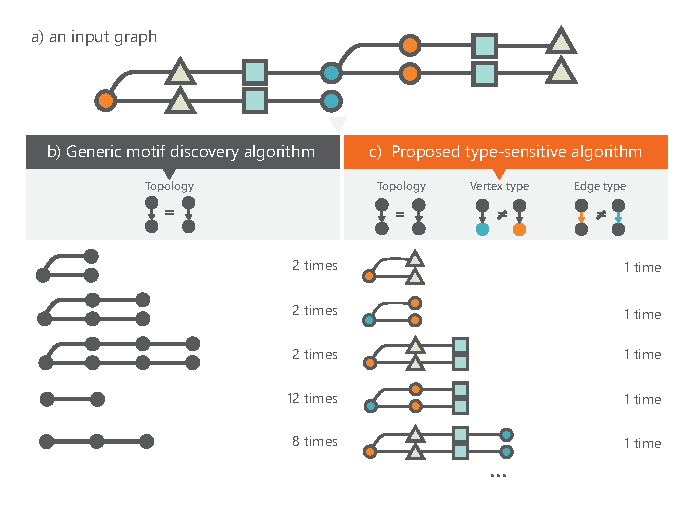
\includegraphics[width=.8\textwidth]{images/automacron/algorithm-differences.eps}
\caption{A) A graph, with typed nodes and edges, where different node types are mapped to different shapes and colours.
B) Generic motif discovery (or search) algorithms focus on topological differences.
C) Our motif extracting algorithm takes varying node/edge types into account, yielding semantically aware motif grouping.
}
\label{fig:new-algorithm-considerations}
\end{figure}

As shown in Table \ref{tab:motif-algorithms}, many motif search/discovery algorithms exist. 
Ribeiro \emph{et al.} \cite{ribeiro10}, Kashani \emph{et al.} \cite{kashani09} and Wong \emph{et al.} \cite{Wong:2012} published benchmarks detailing processing time for a subset of the algorithms in Table \ref{tab:motif-algorithms}.
As subgraph matching is fundamentally an \emph{NP}-complete problem, these algorithms are computationally intensive.
Wong \emph{et al.} report \emph{maVISTO} taking 14,000 seconds to find size three motifs in an \emph{E. Coli} network.
Comparing that to one second for \emph{FANMOD} to analyse the same network, one can see the huge variability in algorithm performance.
As the size of the target motifs grow, performance decreases.
Using the same \emph{E. Coli} network but searching for size 8 motifs, \emph{FANMOD} will need 9,000 seconds to finish the operation \cite{Wong:2012}.

In Table \ref{tab:motif-algorithms} the second column indicates whether the sampling is exact (enumerating all possible candidates) or estimated.
The third column indicates the maximum number of nodes in a motif the algorithm can handle.
The final column indicates whether the algorithm is focused on \emph{motif discovery} (finding repetitive patterns in a set of graphs), or \emph{motif search} (finding a given motif in a set of graphs). 
All algorithms focus on topological patterns in graphs only and do not consider the types of nodes and edges as a search constraint. 
However, the types, or semantic categories of nodes and edges are an interesting property in defining a macro.
There is a more semantically aware motif search algorithm implemented in \emph{VisComplete} \cite{scheideggerquerying2007,koopviscomplete:2008} that compares node labels and node order to predict the next step in a \emph{VisTrails} pipeline analysis over a larger corpus of pipelines.
However this algorithm is topologically less sensitive and provides no way to identify branch/merge events in a motif, or edge types.
A potentially useful algorithm for identifying suitable candidate macros should be type \emph{and} topology sensitive.
This chapter focuses on work to devise such an algorithm, offering additional advantages in computational performance and providing visual mappings with meaningful structural information. 

In our work, when considering whether a subset of steps in a given workflow is the same as another subset in the same or a different workflow, we must consider the semantics attached to each step (see Figure \ref{fig:new-algorithm-considerations}).
Consequently, the task of motif discovery and search is highly constrained by the types of nodes and edges.
Therefore, it is necessary, as well as advantageous, to develop specific motif extraction algorithms for workflow visualizations.
In addition, we propose a novel concept of partially automating the design of macro glyphs.
We consider the use of multi-resolution glyphs to depict macros at different levels of detail when a user interacts with the visualization, a technique referred to by Bederson and Hollan \cite{bedersonpad:1994} and later by Weaver \cite{weaverbuilding2004} as semantic zooming. 

% ==============================
\section{Motivation and System Overview}
\label{sec:Motivation}

Over the past two decades, Biology has benefited from entering the digital era, becoming a data intensive field.
Ancillary to this development, important efforts have been undertaken to preserve and curate digital artefacts in biology, including experimental workflows.
A workflow is a form of directed graph (digraph).
Scientists mainly rely on two types of workflow visualization: digraphs with text labelled boxes or glyph nodes.
The latter enables more compact visual representation than the former \cite{Maguire:2012:TVCG} allowing domain experts to perform their tasks such as error checking and comparison more quickly.
However, workflows can still be quite large and complex, containing many repeated subgraphs, which demand some effort for identification in ``flat'' representations.  
Hence, it is highly desirable to introduce macro representations in workflow visualizations, as both text-based and glyph-based workflow visualizations can benefit from macro-based visual compression.
Although experimental workflows in biology exhibit specific properties that are different from workflows in other disciplines, they often share some characteristics.
Almost all exhibit temporal ordering and most feature only acyclic digraph topologies.
We are therefore hopeful that our algorithm and experience can be transferred to workflow visualizations in other disciplines.

The domain experts involved in this work identified the following requirements: 

\vspace{-2mm}
\begin{enumerate}[itemsep=-1mm]
\item Given a number of workflows, can we obtain the most common patterns/motifs within those workflows?
\item For each motif, can we obtain the occurrence frequencies for that motif and information about which workflows they occur in?
\item Can we automatically create macro representations of those motifs, with the possibility of adding extra annotation to them?
\item Can motif patterns in a workflow be substituted by common macros to make the workflow more compact?
\end{enumerate}

\vspace{-1mm}
Depending on discipline and requirements, macros may be created by individuals based on their own knowledge about needs and usage.
However, such an individualised approach would be impractical if applied to the curation of large collections of experimental workflows as found in data repositories.
Yet, the availability of such data provides an opportunity for the computational identification of commonly occurring motifs in workflows.
The statistics of such motifs offer useful guidance to motif selection when defining macros.

To carry out this work, information was extracted from a curated resource currently holding over 22,000 experimental design workflows (ArrayExpress \cite{ArrayExpress::2012}).
We used a subset of this collection, comprising 9,670 workflows considered to be well-formed with respect to correct connectivity and semantic annotation.
This subset of workflows, available in the ISA-Tab format \cite{rocca-serra10, sansone12}, offers a good representation of experiment typology.
These ISA-Tab files were processed and transferred to a graph database, which provides an optimised environment for storing graph structures and a query language optimised for graph traversal \cite{batra12}. 
For this purpose, we selected \emph{Neo4j} \cite{Neo4J::2012} -- a freely available graph database providing a query language called Cypher, fast traversal algorithms and high scalability (up to several billions of nodes and edges on a single computer).

\begin{figure}[h!]
\centering
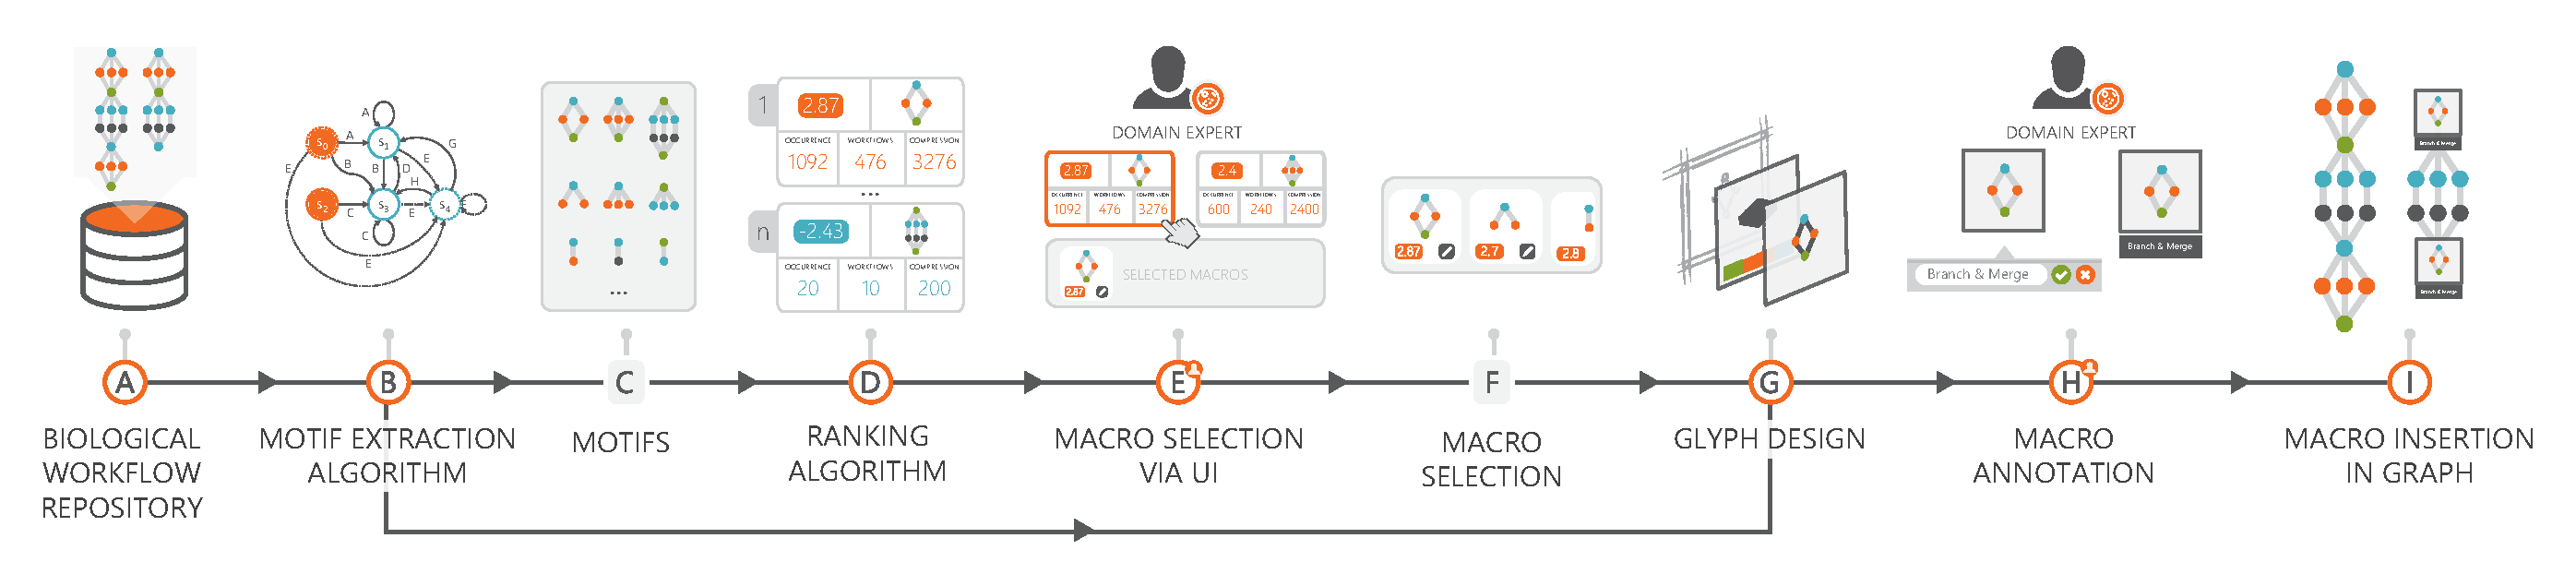
\includegraphics[width=\textwidth]{images/automacron/teaser}
\caption{An overview of the processes implemented in our system, AutoMacron, for compression of workflow visualizations. A) Biological workflows are imported from public repositories. B) The database of workflows is analyzed by our novel motif extraction algorithm that is sensitive to node/edge types and is built using a state-transition approach. C) The algorithm generates a large list of motifs. D) The motifs are ranked using metrics measuring their overall occurrence, scope of influence and compression potential. E) Based on the ordered recommendations by the system as well as their own knowledge, domain experts explore the space of motifs to identify suitable `macros'. F) A subset of motifs are selected for macro generation. G) A glyph is assigned to each macro automatically using a design pattern that utilizes the state output from the motif extraction algorithm. H) Domain experts are able to annotate macros with additional text labels. I) Macros can be inserted into the relevant workflows as a method for graph compression.}
\label{fig:automacron-teaser}
\end{figure}

Our system consists of a number of steps, as depicted in Figure \ref{fig:automacron-teaser}.
\begin{itemize}
\item \textbf{Step 1} (B, C, D) - we algorithmically scan all workflows in the collection and extract all valid subgraphs as candidate motifs.
The patterns and occurrence statistics of these motifs are recorded.
The definition of validity and the extraction algorithm will be detailed in Sections \ref{sec:Conditions} and \ref{sec:automacron_algorithm}.
\item \textbf{Step 2} (E, F) - we provide a user interface for domain experts to define macros by selecting motifs from an ordered list of candidates, based on the statistics computed as well as their domain knowledge about individual motifs and the context of their usage.
This will be discussed in detail in Section \ref{sec:Selection}.
\item \textbf{Step 3} (G, H) - we provide an automatic means for defining the pictogram of a macro by making use of the state transition information captured by the algorithm during the motif discovery phase.
In addition, each macro will normally be displayed with a text label, which is defined by the domain expert through the user interface.
The mechanism for automatic creation of a pictogram will be detailed in Section \ref{sec:Design}.
\item \textbf{Step 4} (I) - we created a tool to allow for substitution of frequent motifs with their macro counterparts in experimental workflows.
This functionality can be accessed via a standalone software package or through an API.
\end{itemize}

% ===============================
\section{From Motifs to Macros}
\label{sec:Motif}

Motif discovery and substitution in graphs typically consists of four processes. These are defined by Milo \etal \cite{Milo:2002} and Alon \cite{Alon:2007} as:

\vspace{-2mm}
\begin{enumerate}[itemsep=-1mm]
\item \emph{Subgraph Generation}: Scan each graph for all possible $n$-node subgraphs.
\item \emph{Motif Amalgamation}: Group together subgraphs that are topologically equivalent and generate a representative subgraph of each group (a motif).
\item \emph{Macro Selection}: Assign a significance value to each motif with respect to other motifs in the collection (for instance, by computing frequency of occurrence) and select the most significant motifs as macros.
\item \emph{Macro Substitution}: Search graphs for subgraphs that match with macros and replace them with that macro.
\end{enumerate}

\vspace{-1mm}
In applications such as biological network rendering, it can be safely assumed that subgraphs should be connected.
By contrast, in applications such as very-large-scale integration (VLSI) design, such a condition is sometimes relaxed, as macros are often used to group elements for a cost-effective spatial placement.
In general, the number of subgraphs can be rather large.
That is why many algorithms only deal with small subgraphs, such as the 4-node subgraphs studied in \cite{Milo:2002}.


\subsection{Candidate Macros in Workflows}
\label{sec:Conditions}
%
The workflows and macros considered in this work exhibit the following characteristics: 

\begin{enumerate}[itemsep=-1mm]
\item A workflow is an acyclic digraph.
\item A macro must consist of at least two nodes.
\item Macros are not only topologically sensitive, but also semantically sensitive. In other words, two subgraphs are said to be in the same motif group only if they are isomorphic and every pair of corresponding nodes (and edges) are of the same type.
\item It is not necessary to have a path between every pair of nodes in a motif.
\item For each node in a macro, there must exist a path from the macro's input node, and a path to the macro's output node.
\item Each macro must have a single input type and a single output type (including \emph{bundled} input and output).
\item A bundled input or output may contain any number of connection edges, but they must be of the same material type.
\item A macro may receive a bundled input converging from different preceding nodes and may deliver a bundled output branching off to different successive nodes.
\end{enumerate}

\begin{figure}[t!]
\centering
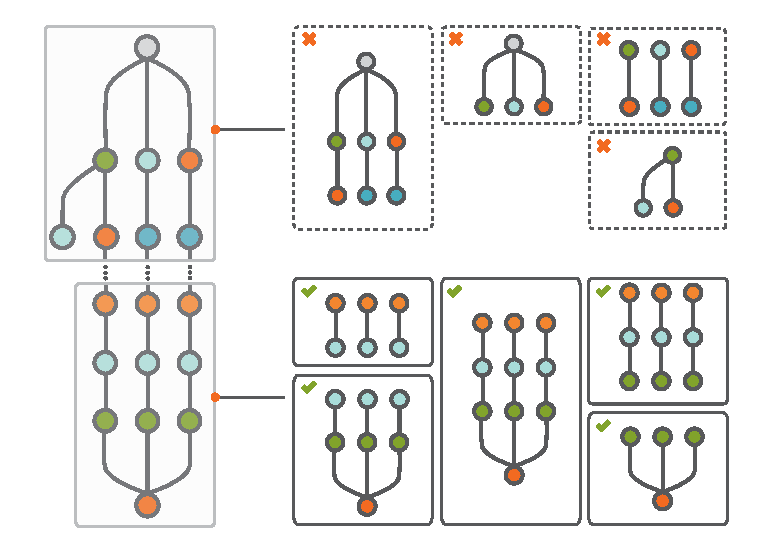
\includegraphics[scale=.6]{images/automacron/valid-invalid-motifs.eps}
\caption{In a workflow graph, some subgraphs can be considered as ``legitimate motifs'' while others cannot, depending on node type. Invalid motifs do not have the same output node type, as indicated by the differing colours. Conversely, valid motifs are those that have the same input and output node type.}
\vspace{-3mm}
\label{fig:Conditions}
\end{figure}


By relying on these characteristics we can significantly reduce the number of subgraphs and motifs to be extracted in the \emph{motif generation} stage of the algorithm.
Figure \ref{fig:Conditions} illustrates those subgraphs that are ``legitimate'' candidates and others that are ``illegitimate''.
In addition, owing to characteristic three described above, the \emph{Motif Amalgamation} and \emph{Macro Substitution} stages are much less onerous in comparison to subgraph matching based on topology only. 

% ---------------------------
\subsection{Motif Generation}
\label{sec:automacron_algorithm}
%
\begin{figure}[t!]
\centering
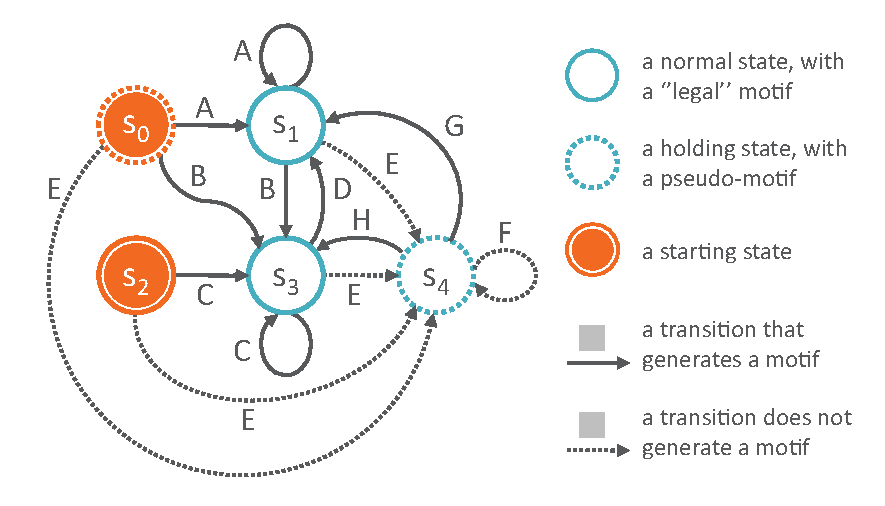
\includegraphics[width=.65\textwidth]{images/automacron/Transition.eps}
\caption{The full space of states and transitions between them encountered during motif generation.}
\label{fig:Transitions}
\end{figure}

\begin{figure*}[t!]
\centering
\begin{tabular}{@{}ccc@{}}
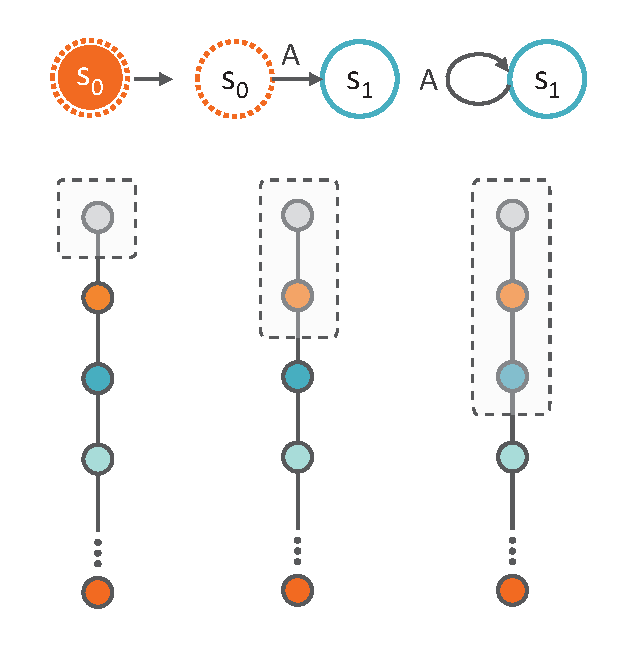
\includegraphics[width=37mm]{images/automacron/States1.eps}&
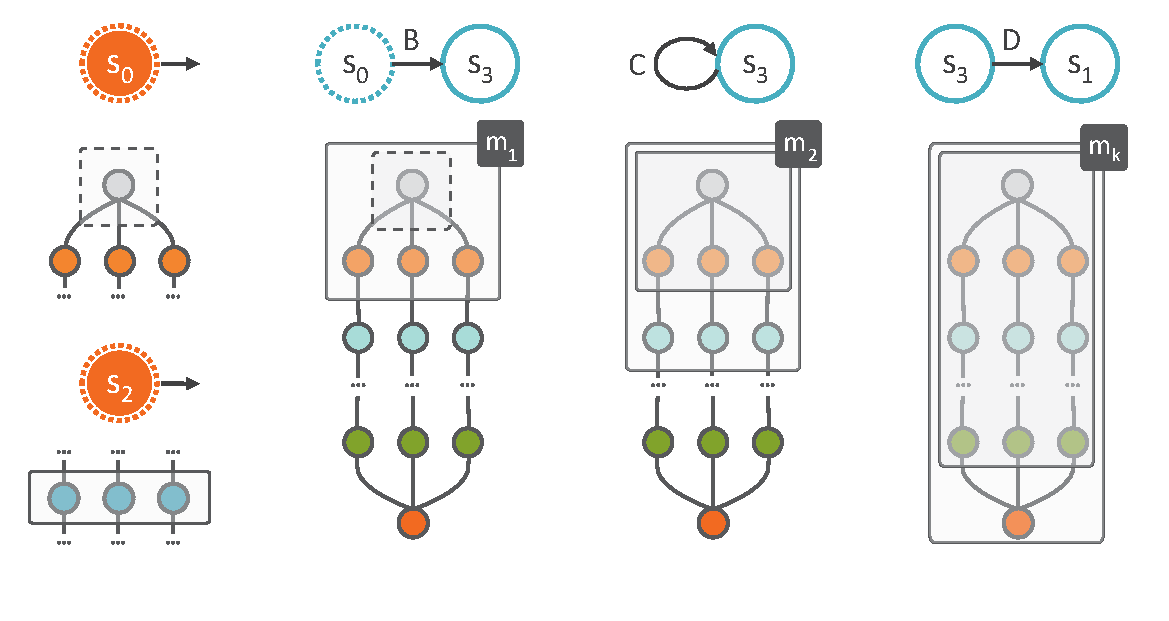
\includegraphics[height=37mm]{images/automacron/States2.pdf}&
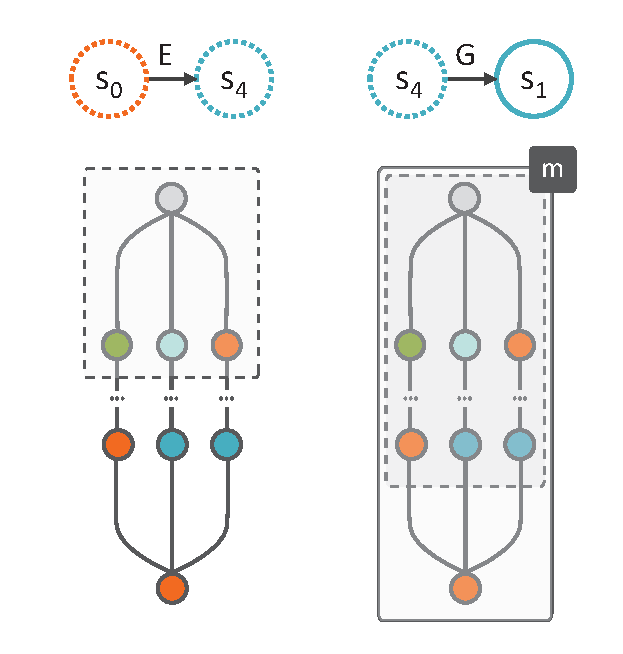
\includegraphics[height=37mm]{images/automacron/States3.eps}\\
A) singular branching & B) homogeneous branching & C) heterogeneous branching
\end{tabular}
\caption{Examples of state transitions with different rules. Homogeneous edges are depicted by using the same colour.}
\label{fig:States}
\end{figure*}

Owing to the aforementioned conditions that are specific to workflows, we could not make use of existing motif generation software and algorithms such as those surveyed in \cite{Wong:2012}.
A specialised motif generation algorithm was needed, and for that we adapted the widely accepted ``pattern growth'' approach \cite{Wong:2012}.
We describe the algorithm by evolving a state transition diagram as shown in Figure \ref{fig:Transitions}.

\noindent \textbf{Singular Branching (Rule A).}
%
As shown in Figure \ref{fig:States} A), the simplest workflow is perhaps a single path composed of $n$ different steps (\eg, experimental steps).
The algorithm can be activated from any node and will only move forward, following the flow of the work.
Since a single node cannot be a macro, the search will park at state $\mathsf{S}_0$ as illustrated in Figure \ref{fig:States} A), where the orange background indicates a starting state and the dotted outline implies that it is only a holding state and does not output a ``legitimate motif''.

When the algorithm encounters the next node $n_1$, it obtains the first ``legitimate motif'', $m_1 = \langle n_0 \rightarrow n_1 \rangle$, and moves to the state $\mathsf{S}_0$.
The edge is labelled with $A$ indicating that this follows rule \textbf{A}.
From $n_1$, the algorithm then encounters $n_2$, it outputs another motif $m_2 = \langle n_0 \rightarrow n_1 \rightarrow n_2 \rangle$, and remains at the same state.
For the workflow in Figure \ref{fig:States} A), this self-loop continues to generate motifs in growing sizes until the end of the path or the number of nodes in the motif reaches a predefined maximum. 

\noindent \textbf{Homogeneous Branching (Rules B, C, D).}
%
One extension of the singular branching case is multiple runs of the same sequence of steps, in parallel.
When the work flows forward, the same type of edges connect to the next set of nodes (see condition 7 in Section \ref{sec:Conditions}).

When an edge first branches to multiple nodes, as illustrated in Figure \ref{fig:Transitions}, the algorithm moves from state $\mathsf{S}_0$ or $\mathsf{S}_1$ to $\mathsf{S}_3$, following a transition of singular branching to bundled homogeneous branching.
This is referred to as rule \textbf{B}.
$\mathsf{S}_3$ indicates more than one edge is being bundled at this state and the number of edges may vary.

The algorithm will self-loop as long as the motif grows with such bundled edges.
Rule \textbf{C} indicates a transition within the state of homogeneous branching.
The number of edges in an edge bundle can change as long as there is more than one edge and they are of the same type.

When all bundled branches converge to a single node, the algorithm returns to state $\mathsf{S}_1$.
This transition is referred to as rule \textbf{D}.
Figure \ref{fig:States} B) shows three examples of applying rules \textbf{B}, \textbf{C} and \textbf{D} respectively.
Applying any of the three rules will result in a bigger motif than the previous one.

An additional state $\mathsf{S}_2$ is included for a scenario when the algorithm starts with a row of parallel nodes with bundled input and output.
We will discuss this scenario later in the context of reactivating the algorithm for bundled edges.

\noindent \textbf{Heterogeneous Branching (Rules E, F, G, H).}
%
Recall conditions 6 and 7 in Section \ref{sec:Conditions}: a macro must have a single input and single output and each can be bundled edges of the same material type.
When these two conditions are met, we can have heterogeneous flow within a macro.
This subset of rules is designed to ``grow'' this particular type of motif.

Rule \textbf{E} is applied when the algorithm first encounters an heterogeneous pattern.
This transition leads to a holding state $\mathsf{S}_4$ and it does not generate any motif.
In this state, all nodes scanned so far are grouped as an interim pseudo-motif and output edges are placed in an interim pseudo-bundle.

The interim state is maintained by a self-loop transition; \emph{i.e.}, rule \textbf{F} as long as the bundled edges remain heterogeneous.
When the edges in an interim pseudo-bundle finally converge to a single node or a set of nodes with homogeneous output edges, the algorithm can leave the holding state $\mathsf{S}_4$.
Rule \textbf{G} defines the transition to singular branching state $\mathsf{S}_1$, while rule \textbf{H} defines the homogeneous branching state $\mathsf{S}_3$.
Both rules will generate a new motif, which includes all nodes in the interim pseudo-motif and the newly encountered node(s).

\noindent \textbf{Termination and Reactivation.}
%
The algorithm strictly follows the breadth-first search strategy.
It may terminate in two situations:
(a) when the predefined maximum depth that a macro may be at is reached;
(b) when it encounters a node without an output edge (\emph{i.e.}, the termination point of a workflow).
The termination condition is tested in all states in Figure \ref{fig:Transitions}.

It is necessary to reactivate the algorithm by choosing each of the different nodes in a workflow as a starting node at state $\textsf{S}_0$.
In addition, each bundle of edges of the same material type can also be a starting point at $\textsf{S}_2$.
Although theoretically appropriate, invoking the algorithm recursively from a starting node of a workflow proved not to be feasible in practice.
We therefore made use of a queue, which initially contains all nodes in a workflow.
We fetch nodes from the queue one at time to invoke the algorithm from $\textsf{S}_0$.
Every time the algorithm reaches state $\textsf{S}_3$, we have a set of homogeneous nodes that were just encountered (\eg, $[n_{1a}, n_{1b}, n_{1c}]$ in Figure \ref{fig:States} B)).
We store all $k$-node subsets of such a set ($k = 2, 3, \ldots$) in a list.
When we finish with all individual nodes in the queue, we sort the list and remove redundant subsets.
We then invoke the algorithm with the sorted and cleaned list from $\textsf{S}_2$.
Note that each subset in the list is a ``legitimate motif'', hence $\textsf{S}_2$ is not a holding state.


% I have to add in the stuff from my meeting with Min here further qualifying why we devised our own algorithm. 

\noindent \textbf{Performance.} To evaluate the performance of the algorithm, we tested it against nine graphs representing biological workflows of varying sizes on a MacBook Pro with a 2.53GHz Intel Core i5 CPU and 8GB RAM.

\begin{figure}[t!]
\centering
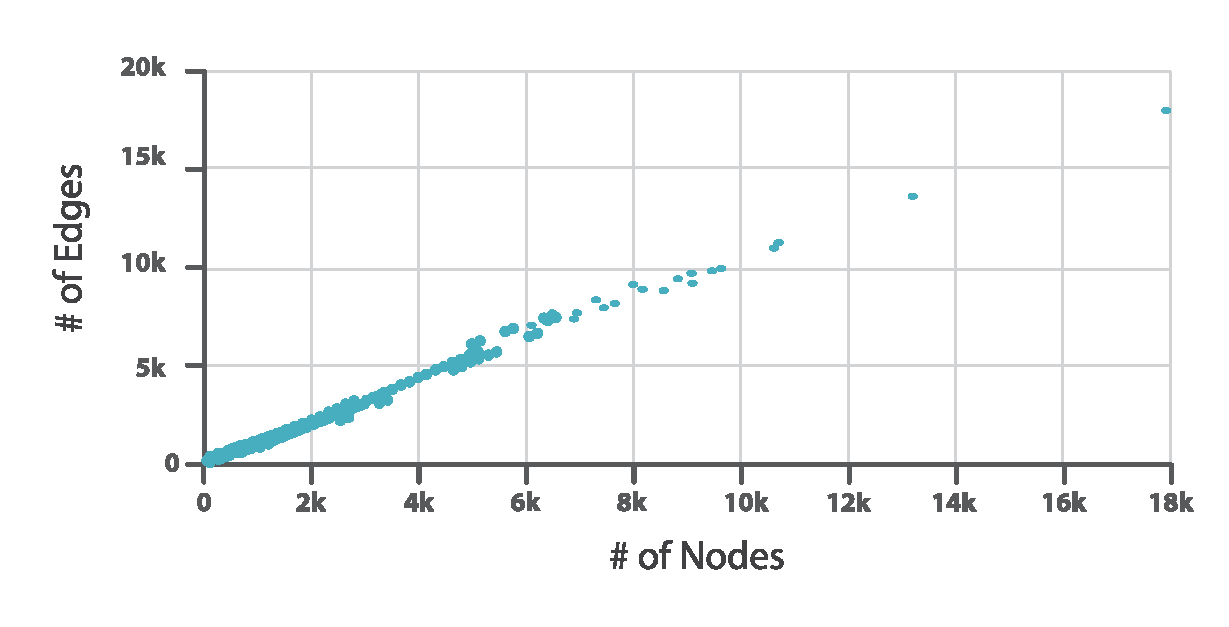
\includegraphics[width=.75\textwidth]{images/automacron/workflow-size.eps}
\caption{Scatter plot showing the distribution of workflows (each depicted as a point) as node count versus edge count.}
\vspace{-4mm}
\label{fig:workflow-size}
\end{figure}


The nine graphs were divided into three groups, three small, three medium and three large, based on their node and edge counts.
Figure \ref{fig:workflow-size} shows the distribution of workflows in our collection in terms of nodes ($x$-axis) and edges ($y$-axis).
93\% of all workflows have a node count below 1,000 and the average number of nodes per workflow is approximately 322.
Given these statistics, we define \emph{small} as 200 nodes or below (covering 58\% of workflows); \emph{medium} between 201 and 600 nodes (covering a further 28\% of workflows); and \emph{large} over 601 nodes (covering the remaining 14\%). 

\begin{table}[t!]
\centering
\vspace{1mm}
\scalebox{0.8}{
\begin{tabular}{|l|r|r|r|r|r|}
\hline
\textbf{Graph Size} & \multicolumn{1}{l|}{\textbf{Motif Depth}} & \multicolumn{1}{l|}{\textbf{G1}} & \multicolumn{1}{l|}{\textbf{G2}} & \multicolumn{1}{l|}{\textbf{G3}} & \multicolumn{1}{l|}{\textbf{Seconds}} \\ \hline
 \multicolumn{ 1}{|l|}{} & 3 & 0.018 & 0.017 & 0.024 & 0.02 \\ \cline{ 2- 6}
\multicolumn{ 1}{|l|}{} & 4 & 0.034 & 0.026 & 0.025 & 0.03 \\ \cline{ 2- 6}
\multicolumn{ 1}{|l|}{} & 5 & 0.048 & 0.038 & 0.042 & 0.04 \\ \cline{ 2- 6}
\multicolumn{ 1}{|l|}{} & 6 & 0.059 & 0.041 & 0.046 & 0.05 \\ \cline{ 2- 6}
\multicolumn{ 1}{|l|}{Small} & 7 & 0.075 & 0.049 & 0.049 & 0.06 \\ \cline{ 2- 6}
\multicolumn{ 1}{|l|}{} & 8 & 0.086 & 0.063 & 0.06 & 0.07 \\ \cline{ 2- 6}
\multicolumn{ 1}{|l|}{} & 9 & 0.095 & 0.064 & 0.062 & 0.07 \\ \cline{ 2- 6}
\multicolumn{ 1}{|l|}{} & 10 & 0.106 & 0.069 & 0.072 & 0.08 \\ \hline
\multicolumn{ 1}{|l|}{} & 3 & 0.153 & 0.065 & 0.056 & 0.09 \\ \cline{ 2- 6}
\multicolumn{ 1}{|l|}{} & 4 & 0.212 & 0.097 & 0.085 & 0.13 \\ \cline{ 2- 6}
\multicolumn{ 1}{|l|}{} & 5 & 0.24 & 0.13 & 0.115 & 0.16 \\ \cline{ 2- 6}
\multicolumn{ 1}{|l|}{} & 6 & 0.293 & 0.161 & 0.138 & 0.2 \\ \cline{ 2- 6}
\multicolumn{ 1}{|l|}{Medium} & 7 & 0.343 & 0.189 & 0.159 & 0.23 \\ \cline{ 2- 6}
\multicolumn{ 1}{|l|}{} & 8 & 0.389 & 0.219 & 0.178 & 0.26 \\ \cline{ 2- 6}
\multicolumn{ 1}{|l|}{} & 9 & 0.429 & 0.241 & 0.183 & 0.28 \\ \cline{ 2- 6}
\multicolumn{ 1}{|l|}{} & 10 & 0.477 & 0.287 & 0.192 & 0.32 \\ \hline
\multicolumn{ 1}{|l|}{} & 3 & 0.296 & 0.756 & 0.354 & 0.47 \\ \cline{ 2- 6}
\multicolumn{ 1}{|l|}{} & 4 & 0.393 & 1.062 & 0.45 & 0.64 \\ \cline{ 2- 6}
\multicolumn{ 1}{|l|}{} & 5 & 0.652 & 1.309 & 0.414 & 0.79 \\ \cline{ 2- 6}
\multicolumn{ 1}{|l|}{} & 6 & 0.632 & 1.528 & 0.42 & 0.86 \\ \cline{ 2- 6}
\multicolumn{ 1}{|l|}{Large} & 7 & 0.75 & 1.829 & 0.341 & 0.97 \\ \cline{ 2- 6}
\multicolumn{ 1}{|l|}{} & 8 & 0.809 & 2.028 & 0.396 & 1.08 \\ \cline{ 2- 6}
\multicolumn{ 1}{|l|}{} & 9 & 0.889 & 2.287 & 0.528 & 1.23 \\ \cline{ 2- 6}
\multicolumn{ 1}{|l|}{} & 10 & 1.047 & 2.489 & 0.604 & 1.38 \\ \hline
\end{tabular}
}
\caption{Performance of our motif-finding algorithm on graphs of varying size and at a range of search depths. 
Averages (last column) are taken across three graphs G1, G2, and G3 in each category. 
For each graph at each depth, the recorded time was the average time over five runs. A more detailed table is available in the supplementary materials.}
\label{tab:performance}
\end{table}

\begin{figure}[ht!]
\centering
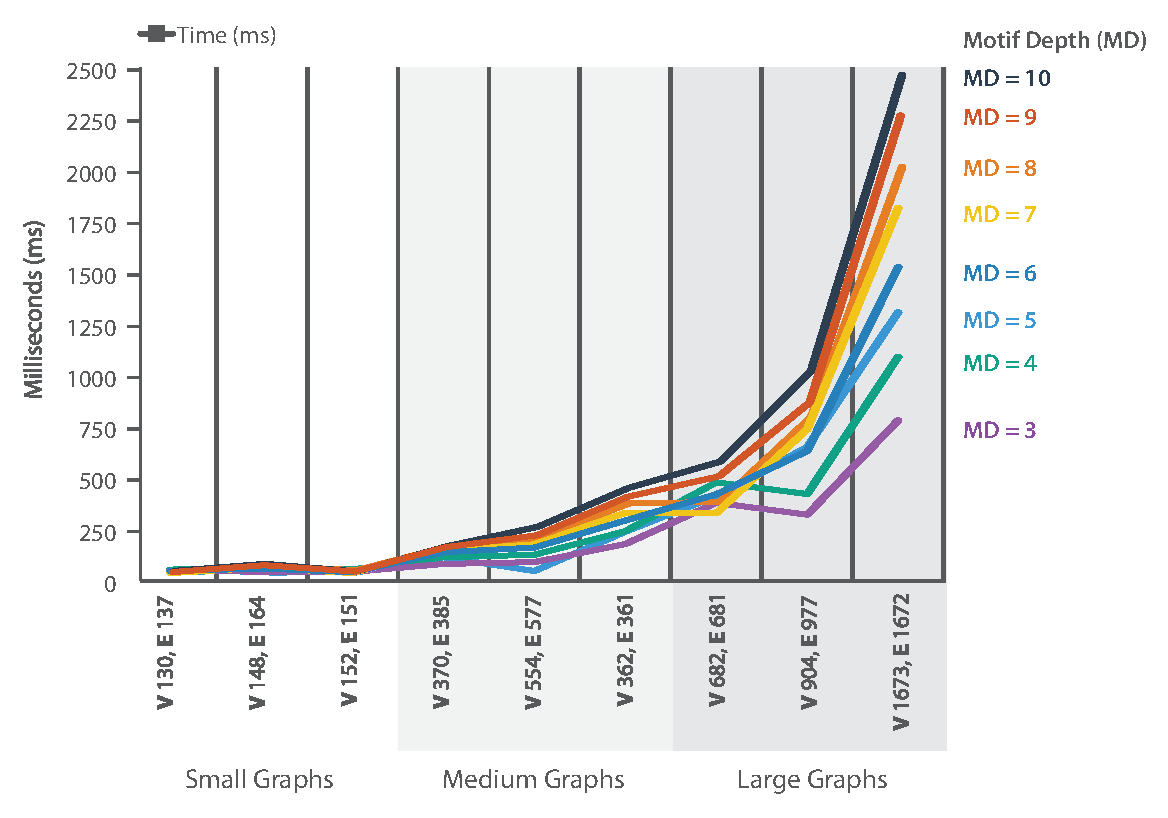
\includegraphics[width=.8\textwidth]{images/automacron/results_graph}
\caption{Overview of our motif finding algorithm's performance at different motif depth cut-offs across small, medium, and large graphs.}
\label{fig:eval_results_graph}
\end{figure}

For each of the nine selected graphs, motifs between a depth of three and ten were searched for, with each search repeated five times to account for any variability.
Table \ref{tab:performance} gives the runtime (in seconds) of applying our algorithm to the nine test graphs.
Results are also summarised in Figure \ref{fig:eval_results_graph}. 
The runtime is scalable to our collection of some 10,000 workflows, as the algorithm runs as a batch process.
It also shows that the speed of our motif finding algorithm compares favourably the current best general purpose motif finding algorithms.

Our algorithm search space differs from the general purpose algorithms listed in Table \ref{tab:motif-algorithms}, since we have introduced specific constraints on motif structure, taking into account the notion of node/edge types.
Nevertheless, we could have theoretically used a two-stage method, by first using a general-purpose algorithm to identity an initial list of motifs, then filtering out those motifs that do not meet our requirements.
Since our algorithm is generally faster than these general purpose algorithms, plus the computation to infer back the node/edge type is potentially large, there is no advantage to using this two-stage approach.


% -------------------------------------
\subsection{Selecting Macros from Candidate Macros}
\label{sec:Selection}

\begin{figure*}[t!]
\centering
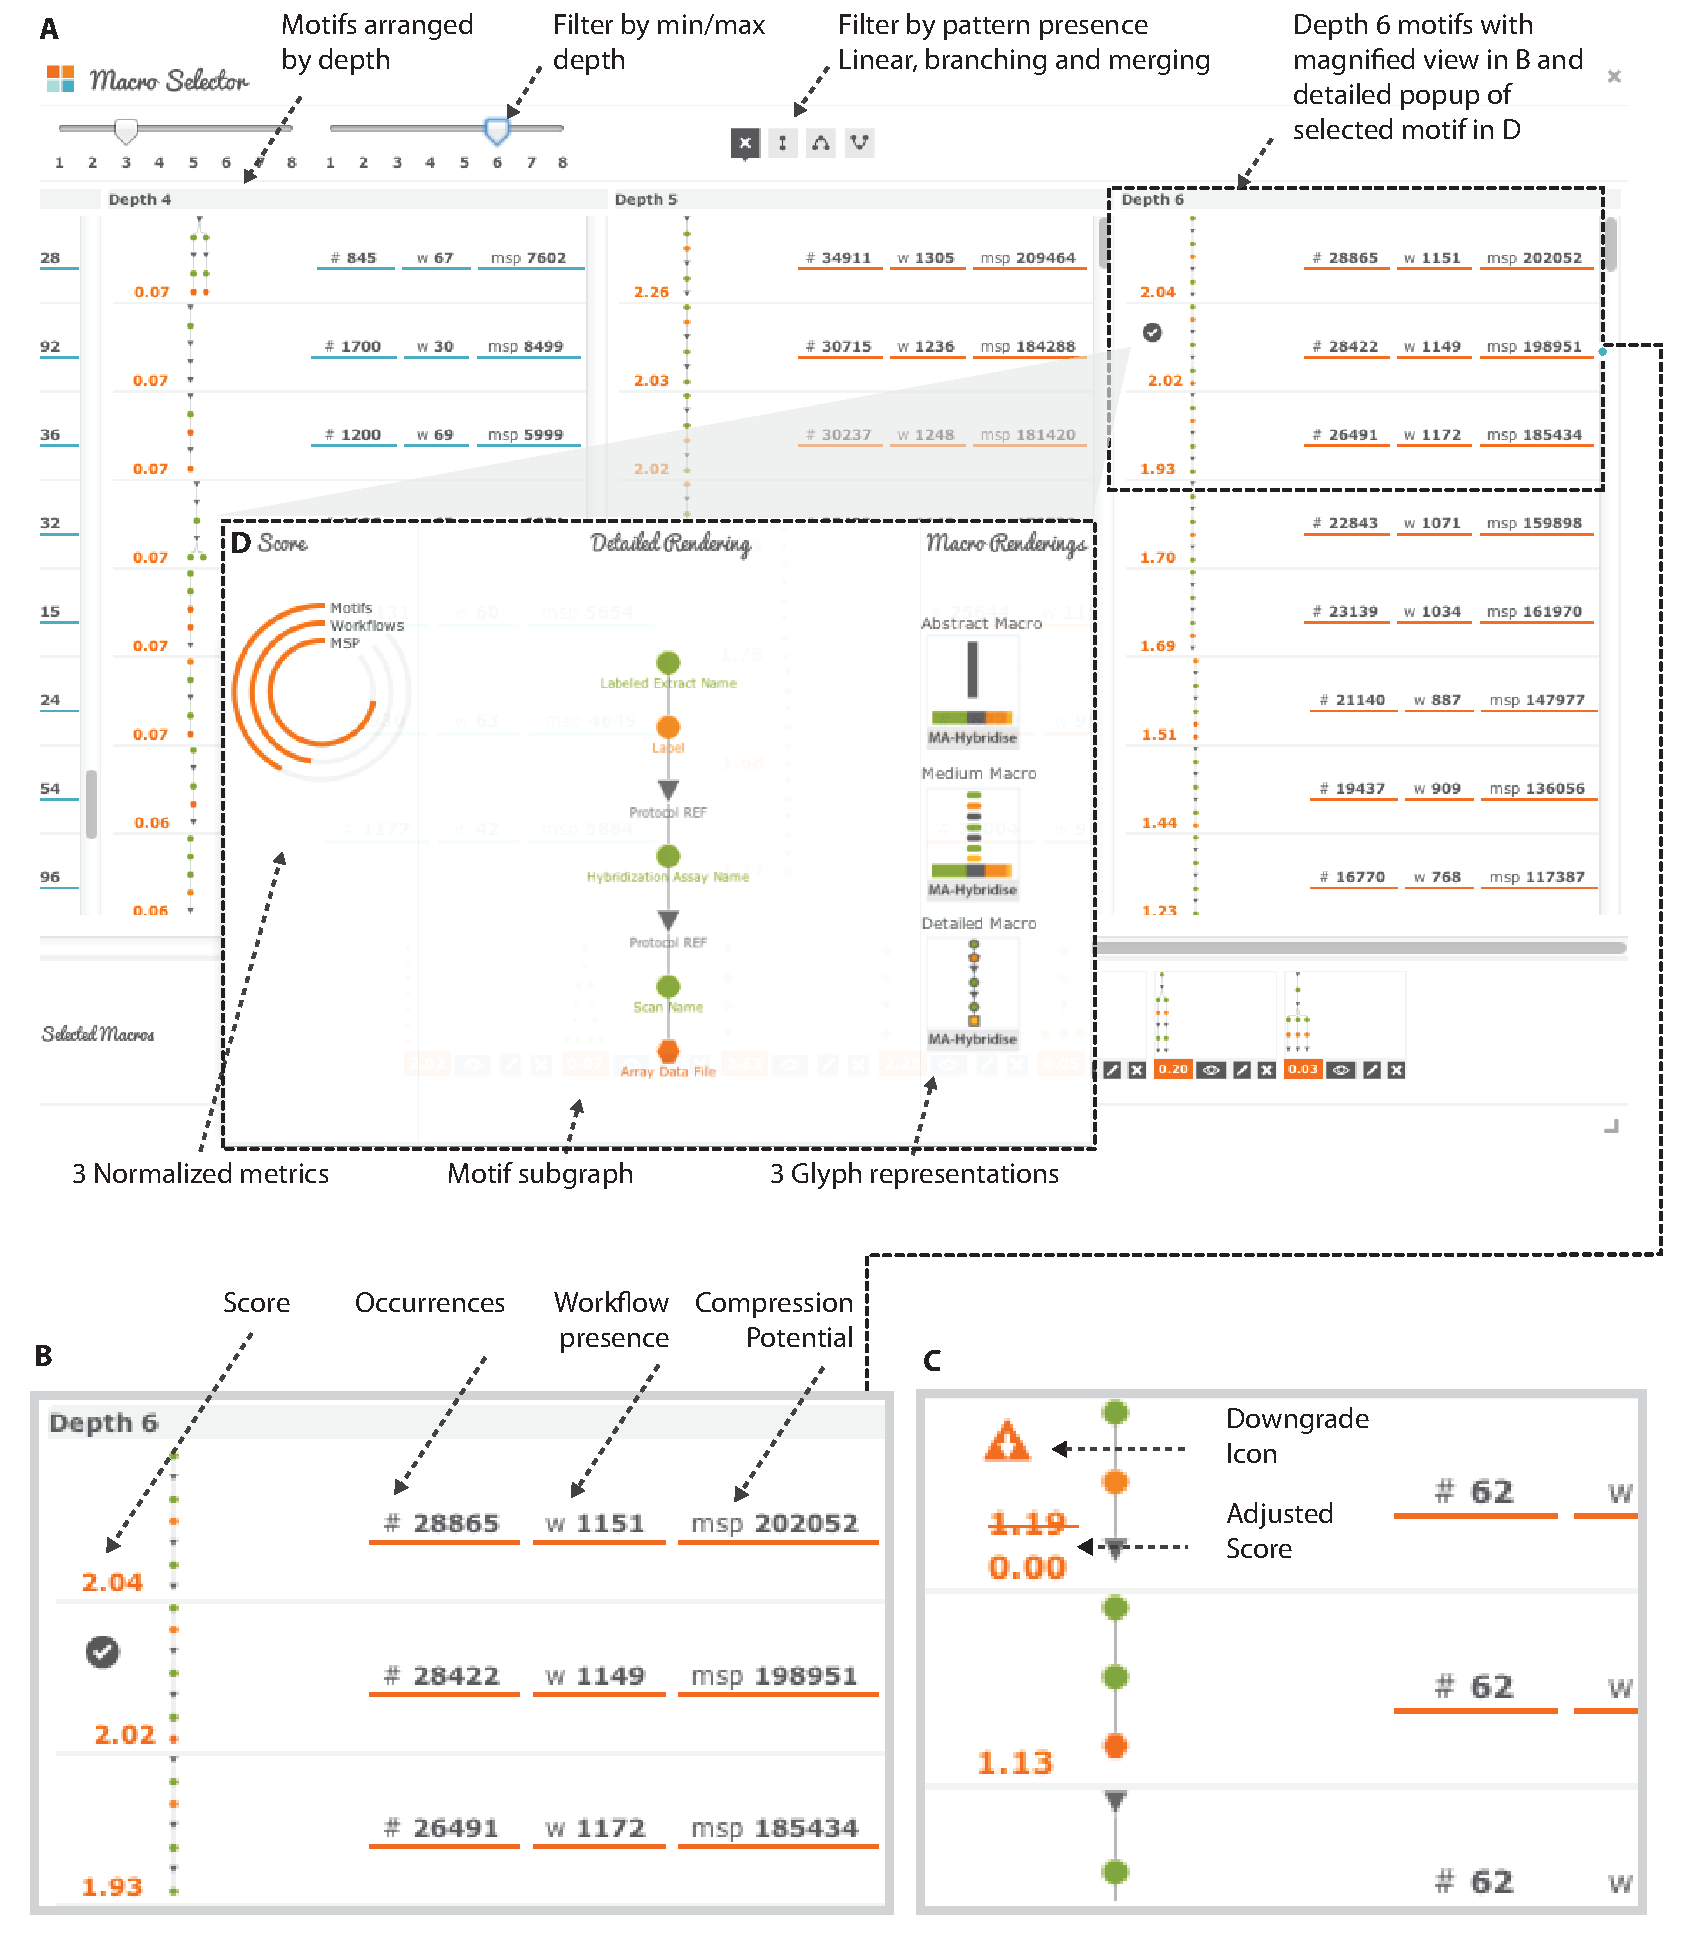
\includegraphics[width=\textwidth]{images/automacron/motif-selection-09}
\caption{AutoMacron provides a user interface (A) for domain experts to select macros from a list of computed motifs.
As shown in the detailed view in (B), the overall score determines the order of motifs in the list.
% The scores are color-coded with higher values (in orange) and lower values (in blue). 
The three indicators are shown in unnormalized form in order to be semantically meaningful.
The detail view (C) shows an example where a score is adjusted dynamically when a motif encompassing other motifs is selected.
(D) shows a pop-up window for a specific macro, detailing its subgraph and three automatically generated pictograms for different levels of details in visualization.}
\label{fig:motif-selection}
\end{figure*}

Given a list of motifs extracted using the algorithm in Section \ref{sec:Algorithm}, we can categorise them into individual groups.
Motifs in each group share the same subgraph topology, and the same set of nodes and edges in terms of their numbers and types.
Each motif group thus becomes a candidate macro.
It is important to emphasise that selecting macros from macro candidates requires a fair amount of knowledge about biology, biological experiments, and the uses of workflows.
In some cases, other information, such as the time when and context in which certain motifs appear frequently, may also feature in the selection process.
Therefore, it is not sensible to make this selection process fully automatic.
In this work, we provide a user interface to assist domain experts in selecting macros from a large list of candidates.

Following the advice of domain experts specialised in biological data curation, we understood the essential requirement for such a user interface is to provide key indicators for each macro candidate $g_i$, including the depth of its subgraph, $A_d(g_i)$, the total number of its occurrences in the data repository, $A_t(g_i)$, the number of workflows that contain it, $A_w(g_i)$, and its compression power $A_c(g_i)$.
For each indicator, normally the higher value the indicator has, the more selectable the candidate is.
However, when the comparison is not clear cut across different indicators, the domain experts will have to make an informed decision based on all the indicators as well as their tacit knowledge about the macro candidate (\eg, biological semantics, importance in science, expected future usage).
As shown in Figure \ref{fig:motif-selection}B, the user interface displays each candidate with these indicators.
The candidates are organised into columns, each representing a specific depth of the subgraphs in all macro candidates. 
Each candidate is shown with the basic pattern along with three indicators, $A_t, A_w, A_c$.
The detailed structure of each macro candidate can be viewed on demand by using mouse interaction.

In order to help domain experts examine a large number of candidates speedily, we sort macros candidates in each column by a ranking score, allowing domain experts to inspect the most promising candidate first.
The ranking score is based on indicator $A_t$, $A_w$, and $A_c$.

\noindent \textbf{Indicator 1: Occurrences in the data repository.} Indicator $A_t$ returns the total number of times a motif has occurred across the entire database of workflows.
It emphasises the importance in selecting motifs that are highly used, inferring their functional importance. 

\noindent \textbf{Indicator 2: Workflow presence.} Indicator $A_w$ returns the total number of workflows in which a motif has appeared.
This provides a measure of how widely a motif is used across different biological experiments, counterbalancing the possible distortion in situations where a motif is heavily used in a relatively small number of workflows. 

\noindent \textbf{Indicator 3: Compression Potential.} Indicator $A_c$ is calculated by first subtracting the number of nodes in the motif ($A_n$) by 1, since these nodes will be replaced by a single macro node, and then multiplying by its occurrence ($A_t$).
It is written as $A_c(g_i) = (A_n(g_i) - 1) * A_t(g_i)$.

For each of these three indicators, we map it to a fixed range $[-1, 1]$ using a linear mapping based on the min-max range of each indicator, yielding three normalised metrics $M_1$, $M_2$, and $M_3$.
These are combined into a single ranking score using a weighted average as:
\[
S(g_i) = \sum_{k=1}^3 \omega_k M_k(g_i)
\]
\noindent where $\omega_k$ are three weights defined by users.
Our system makes no assumptions about the merits of one indicator over another, so the default weights are set to one.
We chose to have the score $S(g_i)$ in the range of $[-3, 3]$, as it helps domain experts to connect the score back to the three indicators.

Figure \ref{fig:motif-selection} shows a screenshot of the user interface on the left (A), and two detailed views with annotation on the right (B, C).
A domain expert normally examines macro candidates with the largest depth value (the rightmost column) first.
Once a motif, $\mathcal{M}$, is selected, it may affect the current results returned by the indicators.
As such a motif, $\mathcal{M}$, may contain many other candidate motifs as subgraphs. It is important for the domain expert to be aware of the impact of this decision on those candidate motifs yet to be examined.
The system thus updates the indicators of all those candidate motifs included in $\mathcal{M}$.
Instead of modifying $A_t$ and $A_w$ directly, the system shows a corrected score calculated by considering the new values for $A_t$, $A_w$ and $A_c$, implying the difference if all $\mathcal{M}$ were to be removed from the repository.

% ====================
\section{Macro Design}
\label{sec:Design}

\begin{figure*}[t!]
\centering
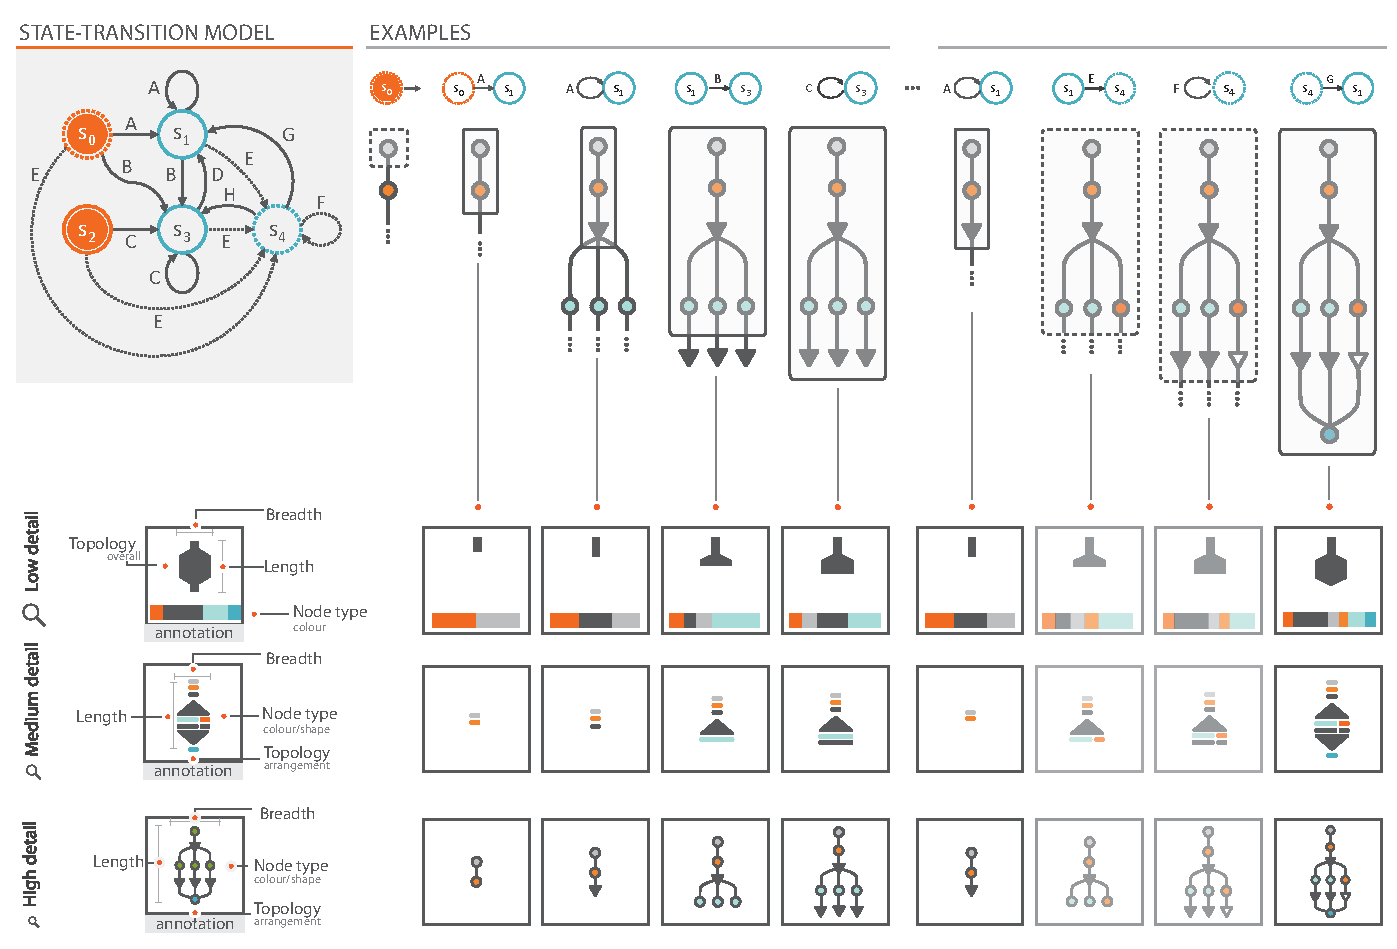
\includegraphics[width=\textwidth]{images/automacron/macro-design-options.pdf}
\caption{From left to right: automatic generation of a micro pictogram based on the state transitions encountered.
The lower three rows: Three design options for representing macros.}
\label{fig:design-options}
\vspace{-3mm}
\end{figure*}

Having obtained a collection of motifs suitable for use as macros within our corpus of workflows, we now have the task of designing their visual representation.
It is important to keep the users in mind and ensure that the design reflects what a typical user, in our case a biologist, would expect to find in a macro. 
We consulted domain experts as to the visual elements that users considered the most important to view.
A number of attributes were identified and are listed below in order of importance:

\vspace{-2mm}
\begin{enumerate}[itemsep=-1mm]
\item an impression of topology/structure within a macro (\eg, it may be an entirely linear path, a set of parallel paths, or it may contain branch/merge events);
\item an impression of types of nodes in a macro (\eg, the overarching theme of the macro);
\item textual description, (\emph{i.e.}, additional annotation to provide concrete semantic meaning and help in understanding);
\item an impression of density within a macro, (\emph{i.e.}, the size of the corresponding subgraph).
\end{enumerate} 

\vspace{-1mm}
Given the attributes listed above, we devised three design options, as illustrated in Figure \ref{fig:design-options}, for creating pictograms.
These pictograms are created automatically based on the states encountered when the motif is found by the motif generation algorithm in Section \ref{sec:Algorithm}.
When the algorithm moves from one state to another, the pictogram grows by adding a new visual component reflecting the subgraph pattern just encountered.
We provide three alternative designs for each macro.
The first option is pixel-based, the second is shape-based and the third is a miniature version of the subgraph.
All three design options are stored as vector graphics, so they are suitable for multi-scale display, for example, through zooming operations.
Textual descriptions of the macros are always provided by experts.


Figure \ref{fig:motif-selection}(D) shows a pop-up window with a detailed view of a macro, and the three design options.
The users can choose to have a fixed design for the macro, or have a multi-scale variation according to the level of detail at which a user is viewing the workflow.

\noindent\textbf{Overview/Low detail}. At the overview level, the fine-grained details of the workflow (\emph{e.g.,} lines) utilise visual channels occupying a high spatial frequency.
It is more effective for nodes in a graph to occupy low spatial frequencies, which will be distinguishable by a user.
The pixel-based design option enables users to use visual channels that are visible and roughly distinguishable in low spatial frequencies.
Although individual nodes and edges are not visible, the user can still gain a rough impression about the topology and node types. 

\noindent\textbf{Medium detail}. At medium detail, users should be able to see more information through the shape-based design.
The major steps from input to output (\emph{i.e.}, following the state transitions) become more distinguishable.
Each horizontal segment of the pictogram is coloured by node type, branching and merging is shown with triangles of mirrored directionality, and heterogeneity of nodes is depicted in separated tracks of differing colours. 

\noindent \textbf{High detail}. When a user zooms into a small region of the visualization, a miniature version of the subgraph becomes available, showing details of the topology and node types. This representation has a lot of high spatial frequency information and is only suitable for detailed examination in close up views.

\section{Software Implementation and Use}

To demonstrate our approach, we developed an open-source Java tool named \emph{AutoMacron} that may be used in two modes: 1) standalone for those wishing to discover common motifs in a database of graphs; and 2) as an API for those wishing to integrate the utilities for motif discovery into their own software.
The software provides the following functionalities:

\vspace{-2mm}
\begin{enumerate}[itemsep=-1mm]
\item Load files that have a handler (\emph{e.g.,} ISA-Tab in our use case) into a graph database;
\item Analysis of all graphs in the database instance to determine the dominant motifs;
\item Allow for selection of macros from the pool of over-represented motifs found by the algorithm;
\item Visualise graphs both in uncompressed/compressed representations, and/or export those graphs in GraphML format for visualization in other environments; 
\item Render differing images depending on the zoom level (semantic zooming \cite{bedersonpad:1994,weaverbuilding2004}). For this, we have extended the Prefuse visualization library \cite{heer05}.
\item Allow for search of a graph database for a user-defined semantically-annotated motif;
\item Export macros for use in other software.
\end{enumerate}

\vspace{-1mm}
Using AutoMacron, over 12,000 valid motifs were found in a collection of 9,670 existing workflows from ArrayExpress. From that set, those motifs scoring below zero with the aforementioned aggregated score $S(g_i)$ were removed from consideration leaving just over 400 candidates. 

Further examination of these candidates was conducted by domain experts using the macro selection utility shown in Figure \ref{fig:motif-selection}.
Examination is aided through both presentation of the metrics and ``live'' highlighting of motif representations as they occur in the original graph representation.
Following the manual selection of 30 of these macros, the domain experts labelled each macro with a textual description, making the corresponding glyphs more meaningful and identifiable. These macros could then be used to substitute the more complex representations in the original graph in an effort to compress the representation.

% talk about insertion in to ISAcreator. Graph database assistance etc. Use of macros can be presented in an easily accessible tool. 

\begin{figure*}[ht!]
\centering
\includegraphics[width=\textwidth]{images/automacron/isacreator-48.eps}
\caption{A) A typical workflow, where a 4-node motif is selected as a macro using AutoMacron. (B) A screenshot of  ISAcreator, which using the AutoMacron API can replace each occurrence of the 4-node motif with its macro representation.}
\vspace{-1mm}
\label{fig:isacreator}
\end{figure*}

Aside from the dedicated \emph{AutoMacron} tool, the motif finding functionalities have been incorporated into ISAcreator, which is a tool used by domain scientists to annotate and curate biological experiment workflows and other necessary documentation. As shown in Figure \ref{fig:isacreator}, the user is given the option to compress an experiment workflow using the macros selected by domain experts for biological data curation. 

\section{Evaluation}

Aided by direct collaboration and regular interaction with domain experts, development of the software followed an evolutionary prototyping process whereby users evaluated the prototype at every major stage of the development. For each prototype users contributed their feedback to the software and algorithm outputs. 

In this section, we summarise the feedback given from the last iteration where we performed the following: 1) analysis of the performance of the algorithm presented in this work in comparison with that of the best existing (and available) algorithm; and 2) observation of how the software met the initial requirements as identified in Section \ref{sec:Motivation} by interviewing expert users.

\subsection{Evaluation Against Existing Algorithms}

\begin{figure*}[ht!]
\centering
\includegraphics[width=.8\textwidth]{images/automacron/evaluation.eps}
\caption{A) A simple experimental graph visualized using the software from Maguire \emph{et al.} \cite{Maguire:2012:TVCG}. In this example, we are showing a specific pattern and how that pattern is represented in both FANMOD and AutoMacron. B) HTML Output for 4-node motifs from FANMOD's analysis identifies 5 motifs with 4 nodes. 2 are incorrect (highlighted in orange) according to our rule set in Section \ref{sec:Conditions}. C) HTML output from AutoMacron's analysis which identifies all 50 motifs. We have highlighted the specific motif being searched for (in blue) matching the highlight pattern in A and B, and show the other serial 4 node motifs (highlighted in grey) that would erroneously be considered the same had it not been for preserved semantics of nodes and edges.}
\vspace{-4mm}
\label{fig:automacron-evaluation}
\end{figure*}

We wished to test the performance of the best in class in existing algorithms with that of the algorithm presented in this work, not necessarily just in speed, but also in what was found and how that compared with domain experts' expectations.
We compared the performance of FANMOD \cite{wernicke06} and the algorithm presented in this work in an attempt to discover which motifs could be found and how they related to the expectations of domain experts.

First, we ran a simple test graph through FANMOD, to detect three, four, five, six, seven, and eight node graphs.
In FANMOD, there is a requirement to run each analysis separately, searching for size 8 node subgraphs does not yield all three to eight node subgraphs.
Figure \ref{fig:automacron-evaluation}B shows the output of a four node motif analysis and highlights FANMODs motif discovery match for a pattern highlighted in Figure \ref{fig:automacron-evaluation}A.
As aforementioned, there is no notion of node or edge type, therefore all four node graphs with the same serial topology will be the same, even though they represent entirely different concepts.
Additionally, FANMOD, typical of the existing class of algorithms, returns invalid results with respect to our definition of a motif as defined in Section \ref{sec:Conditions}.

Following this, we ran the same graph through AutoMacron to generate motifs up to depth eight. Note that FANMODs restriction is on node number (up to eight), whereas our algorithm can have potentially hundreds of nodes at depth eight. Figure \ref{fig:automacron-evaluation} C shows the HTML output from AutoMacron's analysis. The highlighted motif corresponds to those highlighted in Figures \ref{fig:automacron-evaluation}A and B, we magnify the motif to show how our algorithm identifies the exact pattern with topology, node, and edge type preserved.

Finally, we had the domain experts who inspected the graph manually and extracted the motifs they would expect the algorithm to find.
We compared what FANMOD and AutoMacron found with what the user expected.
Our summary results are shown in table \ref{tab:evaluation} with all analysis outputs available at \url{https://bitbucket.org/eamonnmag/automacron-evaluation}.

\begin{table}[!t]
\centering
\vspace{2mm}
\scalebox{1}{
  \begin{tabular}{|c|c|c|c|c|c|c|}
  \hline
  \textbf{Source} & \textbf{Motif Id.} & \textbf{Valid Motifs} & \textbf{Acc} & \textbf{MIdent} & \textbf{UIdent} & \textbf{Time (ms)} \\ \hline
  Domain Experts & 6 & 6 & 100\% & n/a & n/a & n/a \\ \hline
  FANMOD & 73 & 19 & 26\% & 4/19 (21\%) & 5/6 (83\%) & 1030*  \\ \hline
  AutoMacron & 50 & 50 & 100\% & 49/50 (98\%) & 6/6 100\% & 119 \\ \hline
  \end{tabular}
}
\caption{Results of motif identification by the domain experts, FANMOD and AutoMacron. Analysis included: \textbf{MIdent} - the ability of the domain experts to identify motif pictograms generated by the algorithms and match them to the original graph; and \textbf{UIdent} -  the percentage of motifs found by the algorithm with respect to the number identified manually by the domain expert.
Timings for how long it took the domain experts to find motifs was not recorded, hence it's not applicable (n/a) tag.}
\label{tab:evaluation}
\end{table}

The results show that AutoMacron identifies less macros that FANMOD, however if one was to consider all the invalid motifs AutoMacron filters out due to incompatibility with our rule set (see Section \ref{sec:Conditions}), AutoMacron would have reported many more. When we consider just the ``valid'' motifs, AutoMacron has many more than FANMOD (fifty compared with nineteen for FANMOD). 
This is as a direct result of the semantics added by AutoMacron. To illustrate, consider a simple two node directed subgraph ($v \rightarrow v$) with three possible node types ($n$), AutoMacron could theoretically identify $n(n-1)$ different motifs whereas FANMOD and other algorithms already listed here could only identify one.
Figures \ref{fig:automacron-evaluation} B and C show for instance how one 4-node motif found in FANMOD maps to five potential, but only one correct motif in AutoMacron. Overall both algorithms identified the majority of motifs expected by the user, not unexpected considering both mechanisms are exhaustive, however FANMOD struggled when it came to identifying the larger motifs, due to the node limit of eight, hence its UIdent value of 83\%. 

The user was also asked to identify motifs based solely on the pictograms representing topology (macros) output from each program.
In 98\% of occasions, the user could identify AutoMacron motifs, aided by both colour coding and better topological arrangement.
With FANMOD however, the user was able to decode 21\% of the outputs. 

\subsection{Evaluation Against User Requirements}
%
The algorithm and tool were tested by two biologists from the University of Oxford who were also authors on the resulting paper (Dr. Susanna-Assunta Sansone and Dr. Philippe Rocca-Serra).
Our tests served to determine how the software has met the four requirements identified in Section \ref{sec:Motivation}.
For each requirement, we summarise their feedback below.

\vspace{-2mm}
\begin{enumerate}[itemsep=-1mm]
\item Given a number of workflows, can we obtain the most common patterns/motifs within those workflows?
  
    \emph{We tested AutoMacron on nearly 10,000 workflows, the software returned an abundance of motifs that were sorted by a score. The filtering tools helped us in finding motifs with specific topological events.}
  
\item For each motif, can we obtain the occurrence frequencies for that motif and information about which workflows they occur in?
  
    \emph{For each motif reported by the software, we were able to recover statistics about how often the pattern occurred as well, how many workflows the pattern appeared in and the names of these individual workflows.}
  
\item Can we automatically create macro representations of motifs with the added ability to add extra annotation?
  
    \emph{Each motif had three variations of macro representations created automatically that could be used depending on the resolution available. We were able to add small pieces of text to these to help identification of the function of these macros, \eg labelling, extraction, or scanning.}

\item Can motif patterns in a workflow be substituted by common macros to make the workflow more compact?
  
    \emph{The software provides a function to show compressed views of a workflow which automatically substitutes motif patterns with their macro representation. The function was also integrated to ISAcreator allowing us to serve out compressed representations of workflows to our users.}
\end{enumerate}

\vspace{-1mm}
Further to this, users added that the software allowed them to identify erroneous annotations very quickly.
For example, through inspecting the motifs, one domain expert discovered a prominent motif with nodes in the wrong position.
This was only detectable via the algorithm's ability to maintain node type.
On this matter, the domain expert commented ``\emph{Being able to detect such errors in annotation so quickly has enabled us to build scripts to fix those records and improve annotation quality.
We can use this tool to find and fix inaccuracies in biological workflows much more quickly than we could before.}''

In many ways, the domain experts regard AutoMacron as a time-saving tool.
Macro glyphs have a similar function to traffic signs.
Domain experts normally expect certain macro glyphs in certain workflows.
Although glyphs are small, they provide more assurance than observing detailed subgraphs directly because macros are computationally determined.
It has helped them to construct the motif space computationally, which would otherwise takes years of effort.
It has enabled them to explore the space of motifs efficiently with the aid of the ordered recommendations by the system.
It has allowed them to create macros quickly without the need to design a pictogram for each macro.
In the medium term, their everyday tasks, such as error checking, comparison, and identifying best practice, can be performed more speedily.
In the long run, they also hope that this will bring benefits to the wider community; for instance, in experimental documentation and scientific publication.

While the discipline of biology has led the way in collecting workflows as part of data curation and sharing, we anticipate that some other disciplines will follow this trend soon.
Our approach to workflow visualization in general and macro generation in particular can be adapted for other types of workflows if they have been curated.

A video of our tool, including feedback from our domain experts is available from \url{http://vimeo.com/71495896}.
 
\section{Contributions}

In this work, we introduced a new approach to macro creation aimed at reducing visual complexity in workflow visualizations using glyphs.
We developed a novel algorithm to discover motifs, with discrimination of node and edge type in a large collection of graphs.
The algorithm was specifically designed for motifs in workflows and performed more efficiently than general-purpose motif finding algorithms. 

We used a statistically-informed approach and an intuitive user interface to help domain experts select macros from motif candidates.
A novel design method for automated creation of glyphs to represent macros was devised by making use of the state transition information obtained from the motif discovery algorithm.
Our glyphs were developed to take into consideration knowledge from Chapter \ref{chap:related_work} regarding spatial frequencies and global/local processing to ensure that the most important information for macros was always available, even at the overview level of the visualization.

These methods were implemented in a software system available through a dedicated graphical user interface (GUI) or an API.
Our domain experts were able to use the system both to generate macros for compression of workflows and to find errors in a large corpus of existing workflows.
Additionally, the selected macros and graph substitution algorithms are integrated into the ISA tools suite \footnote{\url{http://www.isa-tools.org}} used by a large body of experimental biologists as part of the ISA commons \footnote{\url{http://www.isacommons.org}}.

This work was published in IEEE TVCG in a publication by Maguire \etal \cite{maguire13} and presented in the InfoVis track at IEEE VIS 2013.
 


\chapter{Future Work}
\chapter{Conclusion}
\label{chap:conclusion}

\begin{chapquote}{Roger Bacon}{``Reasoning draws a conclusion and makes us grant the conclusion, but does not make the conclusion certain, nor does it remove doubt so that the mind may rest on the intuition of truth, unless the mind discovers it by the path of experience.''}
\end{chapquote}

Glyph-based visualizations can provide real benefits when their corresponding glyphs are properly designed.
However poor glyph design will present limitations to the utility of such visualizations \cite{morris2000experimental, ward02}.
This thesis set out to explore how glyph design could be made more systematic through addition of processes that could reduce subjectivity present in a number of areas including:
the mapping process between data and visual encodings, and the arrangement of these encodings within a glyph; 
the design of glyph libraries for glyph-based visual compression; and
glyph evaluation.

As part of our exploration of the problem space, we proposed a model for systematisation in Chapter \ref{chap:strategies} that placed computational techniques and design principles as core components in the glyph design process.
While this model represented a number of strategies for systematic glyph design using computation, it was also flexible enough to consider cases where computation was not always applicable, such as the biological sequence logo and initial poetry glyph design in Chapter \ref{chap:processes}.

More importantly, through use of this model, we were able to devise strategies to investigate the research questions from Chapter \ref{chap:introduction}.
The contributions of this thesis can be summarised through answers to those questions.

\section{Contributions}
We state the contributions of this thesis through focusing on the questions from Chapter \ref{chap:introduction}.
Is glyph design amenable to systematisation by computational methods?
Can computational methods be applied to the design of glyph libraries?
Is glyph evaluation amenable to systematisation by computational methods?

% \begin{figure}[!ht]
%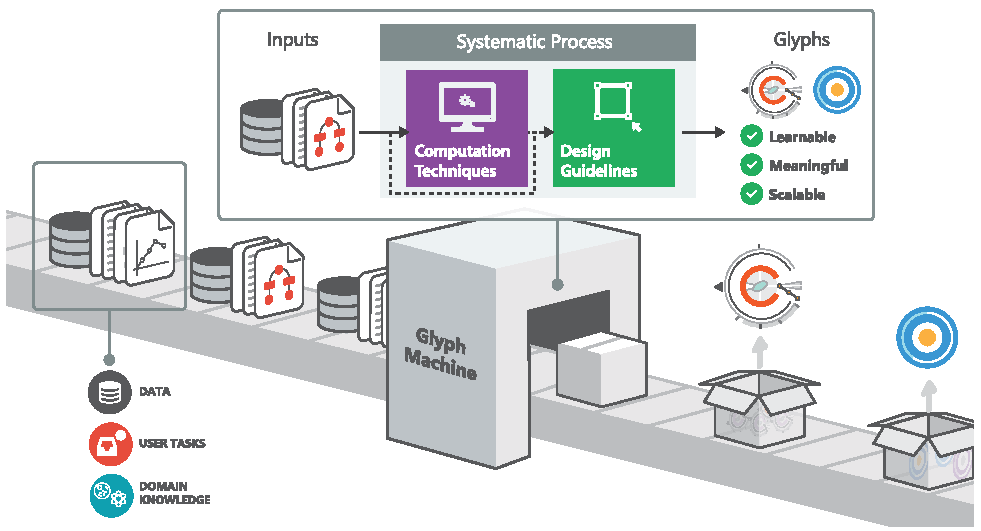
\includegraphics[width=\textwidth]{images/conclusion/systematic_design}
%\caption{Towards a systematic glyph design.}
%\label{fig:systematic_design}
%\end{figure}

\subsection{Is Glyph Design Amenable to Systematization by Computational \\Methods?}
Glyph design is bound by a number of properties of the human perception system.
In Chapter \ref{chap:related_work} we showed how it is bound by our capacity to perceive high spatial frequencies at low resolutions, by limits in how we perceive colour (hue and saturation), size, length, orientation.
Our interpretation of a visual channel is also bound by our ability to remember mappings from data to the visual channels we use to represent them.
This is why use of natural mappings, in particular metaphor, is important.

To move this knowledge to a more actionable form, we devised a number of design principles that summarise some of the more important points to consider when creating glyphs, including:
1) channel suitability;
2) natural/semantic mappings;
3) visual hierarchy (this also dictates the ``power'' of the visual channel to be used);
4) channel composition;
5) channel capacity; and
6) use of redundant encodings for important data.

While application of these principles can provide a level of systematisation, we also wished to investigate how computational approaches could remove the subjectivity in forming the visual hierarchy for instance.
A major contribution of this thesis was the creation of such a computational approach.
Our taxonomy-based approach to glyph design in Chapter \ref{chap:glyph-tax} showed for the first time how numerous components of glyph design could be informed through computation.
The taxonomy algorithm provided a hierarchical organisation that could categorise items to be represented as glyphs.
This hierarchical structure provided the basis for construction of the visual hierarchy.
The stronger visual channels, \eg, colour hue, were selected for higher levels in the taxonomy so that they could be distinguished at even low resolutions.
Less strong visual channels occupying higher spatial frequencies were mapped to lower levels in the taxonomy.

Additionally the algorithm for taxonomy generation selects for schemes that have a small number of categories (less than eight) to reduce the probability of exceeding the capacity limits of a visual channel.
The lower the number of values to be represented by a visual channel, the fewer difficulties there are in memorising and learning abstract mappings to colour or shape for example.
Moreover, a few number of values represented by a visual channel can mean a reduction in the chance of interpretation errors due to a greater distance between shapes, colours, line width, and so on.

A further example of how computational approaches can help glyph design was demonstrated in Chapter \ref{chap:processes} Section \ref{sec:poetry}.
Here, computation was used to assist the design of static and dynamic macro glyphs for poems.
We showed how structural and statistical analysis of a graph created from vowel sounds and their transitions in a poem could inform how the corresponding glyphs are composed.

\subsection{Can Computational Methods be Applied to the Design of Glyph Libraries for Visual Compression?}

Another important aspect of glyph design is deciding what to represent with glyphs to aid better visual search for events in graphs, time-series, or text data for example.
Similar to traffic signage where a number of text-based signs were converted to more iconic representations to certain events easier to see, it would be convenient to replace commonly observed patterns in a visualization with more compact glyph representations that are easier to visually search.
Meanwhile, the remainder of the visualization is left in its original form since it may be regarded as more anomalous.

A further contribution of this thesis is in the application of computational methods to enable more systematic design of glyph libraries.
Our process focuses on the use of data and statistics to suggest motifs that are candidates for visual information compression.
From these statistically informed suggestions, domain experts can filter out semantically meaningless patterns to create a semantically, and statistically informed glyph library.
To apply this process, we focused on visual compression of the workflow graphs from Chapter \ref{chap:glyph-tax}, and time series data.

First, we applied this systematic approach to graphs in Chapter \ref{chap:automacron}.
We developed a novel motif finding algorithm that considers node and edge semantics as well as topology.
This motif detection algorithm was run on nearly 11,000 studies and approximately 500,000 individual experiments to determine common structures across a representative sample of the data.
Results were presented to domain experts, and sorted on a summary score composed through use of a number of metrics.
Experts were then able to select motifs to form a glyph library for compression.
Additionally, the creation of multi-resolution glyphs (different details for different zoom factors) was automated through use of the state transition model that underpins the motif detection algorithm.

Next, in Chapter \ref{chap:timeseries} we applied this approach to time-series data.
A data-driven approach was again used where our algorithm takes a collection of time-series, statistically analyses these for common patterns, and presents the resulting patterns back to domain-experts.
Domain-experts are again in the loop to ensure that motifs are semantically relevant.

Both pieces of work have shown that a computational approach to glyph selection can work to systematise selection of motifs for glyph-based compression.
Human intervention is not removed completely, but decisions are more informed through the statistics we have introduced.

\subsection{Is Glyph Evaluation Amenable to Systematization by Computational \\Methods?}
Numerous aspects of glyphs can be evaluated, some will be domain dependent, others are more general.
For example, if glyphs are designed to encode complex cardiology data, it will be hard to assess the utility of such a glyph without input from domain experts.
 
More general types of evaluation however, such as evaluating the discriminability of a glyph, can be assessed computationally as shown in our work in Chapter \ref{chap:processes} Section \ref{sec:file_system}.
This computational approach is underpinned by a new metric to measure glyph distinguishability, named the quasi-Hamming distance (QHD).
We tested this metric by measuring the distance between visual stimuli using both human participants and an image similarity algorithm.
Our computationally-obtained distances were shown to be well correlated with user-based results.

\section{Summary and Future Research Directions}

The work presented here opens up a number of interesting research avenues around glyph-design.
While we can see that glyph design has gained more popularity in recent years \cite{Polk14, kachkaev2014, CGF:Abd2013a}, creating well designed glyphs for an effective glyph-based visualization can be difficult, especially glyphs like those given in Chapter \ref{chap:glyph-tax}.
For example, scatter plot matrices and parallel coordinate plots simply require a user to load comma-separated value (CSV) files representing the data, and the visualization is rendered.
For a glyph-based visualization we first need examples of the data to be represented, glyphs will be designed around this data, and finally, those glyphs need to be positioned in a display.
The systematic approaches presented in this thesis go some way to simplifying the design step, but more needs to be done to make the process even simpler for users, making it as easy to create effective glyph-based visualizations as it is to create parallel coordinate plots.

Future research directions should build upon the techniques presented in this work and drive towards more automatic glyph design and evaluation.
This would make glyph-based visualizations for data exploration something that any user could deploy.
The path towards such a vision lies in what I believe to be a number of future developments:
\begin{enumerate}
\item \textbf{A glyph encoder/decoder} illustrated in Figure \ref{fig:encode_decode} that would extend on this thesis to investigate both how automatised encoding of glyphs can be accomplished, and how much ``information'' could be decoded from glyphs.

\begin{figure}[t!]
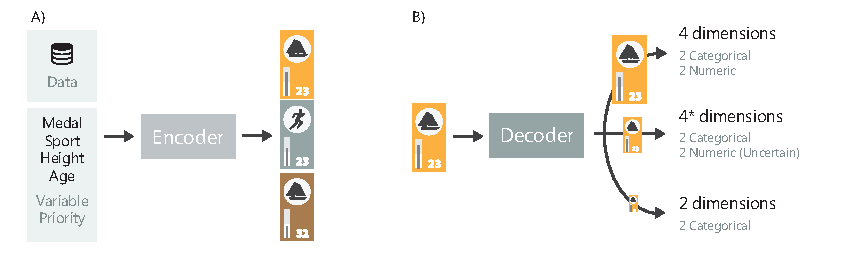
\includegraphics[width=\textwidth]{images/conclusion/encode_decode}
\caption{A) A glyph \emph{encoder} can take a set of data, with variable priority and automatically create glyphs for the data.
B) A glyph \emph{decoder} can take a glyph, automatically ``crush'' it to test different resolutions, and output how many pieces of distinct pieces of information are visually available.}
\label{fig:encode_decode}
\end{figure}

For this to happen, a number of research directions would need to be investigated:
\begin{enumerate}
 \item \textbf{Encoding} in Figure \ref{fig:encode_decode} A) is made difficult due to the metaphoric requirements in many glyph designs.
Metaphor has been mentioned many times in this thesis due to its importance in making it possible to remember mappings between concrete concepts and colour, shape, or texture for instance.
In essence, glyphs are easier to decode if their form maps more directly on to reality.
Recently, Lin \etal \cite{lin2013selecting} presented a promising step towards automated metaphoric colour generation through computational creation of semantically-resonant colours using Google search results.
An interesting future direction could be in building a tool to automatically create semantically-resonant shapes using a similar approach.

Additionally, further research is required to investigate the integrality and separability of dimensions in glyphs rather than solely focusing on visual primitives; and

\item \textbf{Decoding} in Figure \ref{fig:encode_decode} B) would require better image decomposition and area identification within images to find ways of decoding parts of a glyph.
Such a system would automatically decompose glyphs and predict the underlying data type.
For example, when a scale is detected or numbers are present, the data type is likely to be numeric.
If colours occupy distinct hues or if shape is used, the data is likely to be categorical.
Additionally, as part of the decoding process, glyphs would automatically be ``crushed'' to simulate what could be viewed at different resolutions and ensure that important information is always available, even at lower resolutions.
\end{enumerate}

\begin{figure}[t!]
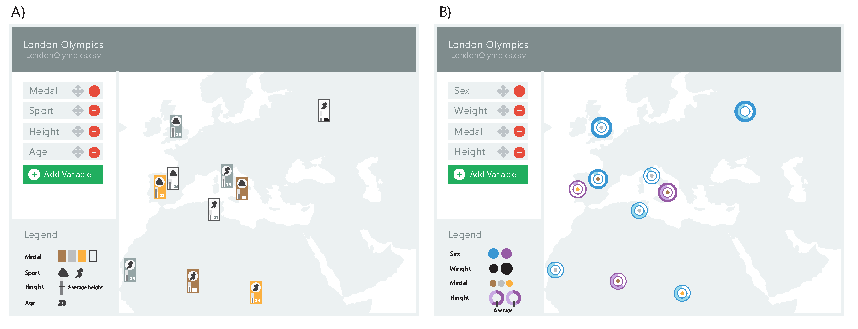
\includegraphics[width=\textwidth]{images/conclusion/glyph_exploration}
\caption{Glyph-based exploration of athletes competing in the London 2012 olympics.
A) Medal and sport are the most important variables for the task.
Less important visual variables such as height and age can be retrieved on closer inspection by zooming in.
B) Gender and weight are now the most important variables for the exploration task, resulting in a different glyph representation.}
\label{fig:glyph_exploration}
\end{figure}

An efficient encoding tool would present a path towards automatic glyph creation, extending on the \emph{GlyphMaker} work from twenty years ago by Ribarsky \etal \cite{ribarsky94}.
The decoding tool would help automatically validate a glyph design by measuring its effectiveness in terms of detecting how much information is available to a user at different resolutions, and what that information is.
Together, these would lay down a path for automatic glyph design (and validation), contributing towards a general-purpose glyph-based exploration library.

\item \textbf{Glyph-based data exploration} that would make glyph-based visualizations as easy to instantiate as parallel coordinates or scatter plot matrices.
Given a process for automated glyph creation exists, it should be possible to create task driven glyph-based visualizations that automatically change depending on the details a user felt most important in their analysis.
An example of how such a system may look is shown in Figures \ref{fig:glyph_exploration} A) and B) that show an interface whose glyphs change depending on the variables used and the ordering of their importance.

\item \textbf{Better quality measures} for glyph-based visualizations that extend on our quasi-Hamming distance metric introduced in Chapter \ref{chap:processes} to determine glyph distinguishability.
While glyph utility and memorability may not be suitable for assessment using computation, glyph interpretability could perhaps be measured using such an approach.
\end{enumerate}



% Appendices
%\appendix
%\include{appendices/pseucode.tex}
\listoffigures
\addcontentsline{toc}{chapter}{Bibliography}
\bibliography{thesis}
\bibliographystyle{amsalpha}

\end{document}

